\documentclass{article}
\usepackage[utf8]{inputenc}
\usepackage[english]{babel}
\usepackage[T1]{fontenc}
\usepackage{graphicx}
\usepackage{listings}
\usepackage{xcolor}
\usepackage{multicol}
\usepackage{float}

\usepackage{xcolor}
\newcommand\crule[3][black]{\textcolor{#1}{\rule{#2}{#3}}}

\definecolor{codegreen}{rgb}{0,0.6,0}
\definecolor{codegray}{rgb}{0.5,0.5,0.5}
\definecolor{codepurple}{rgb}{0.58,0,0.82}
\definecolor{backcolour}{rgb}{0.95,0.95,0.92}

\lstdefinestyle{mystyle}{
    backgroundcolor=\color{white},   
    commentstyle=\color{codegreen},
    keywordstyle=\color{magenta},
    numberstyle=\tiny\color{codegray},
    stringstyle=\color{codepurple},
    basicstyle=\ttfamily\footnotesize,
    breakatwhitespace=false,         
    breaklines=true,                 
    captionpos=b,                    
    keepspaces=true,                 
    numbers=left,                    
    numbersep=5pt,                  
    showspaces=false,                
    showstringspaces=false,
    showtabs=false,                  
    tabsize=2
}

\lstset{style=mystyle}

\title{
	{Performance Evaluation of a Deficit Scheduler}\\
	{\large Università di Pisa\vspace{1cm}}\\
	{
\includegraphics[scale=.5]{images/Stemma_unipi.png}}
}
\author{Pezzuti Francesca \and Sanguinetti Marta \and Vivani Alessio}
\date{Academic year 2021/2022}


\begin{document}

\maketitle

\newpage

\tableofcontents

\newpage

\section{Introduction}
    Our project consisted in the implementation and performance analysis of a deficit scheduler. There is a source sending jobs to a server. Job inter-arrival times are IID RVs and their service times are IID RV. The server serves jobs in the queue automatically and service occurs within one turn. The expected time that the server should spend on the source is Q. However:
    \begin{itemize}
        \item If the queue is empty, the turn is terminated.
        \item If the next job cannot be served entirely before the end of the turn, the turn is terminated and the remaining time (called deficit) is saved and summed to the duration of the next turn. If the deficit is equal to D then the next turn will be Q+D units of time.
    \end{itemize}
    After a turn, the server then \textit{goes on vacation} for some time. Vacations are IID RVs. If a server comes back from vacation and finds the queue empty, it immediately starts a new vacation.

\newpage

\section{Simulation}
    We used OMNeT++ to simulate our system, exploiting NED to implement the structure of the system and C++ to define the behavior of each component.
    \newline
    \begin{figure}[ht!]
        \centering
        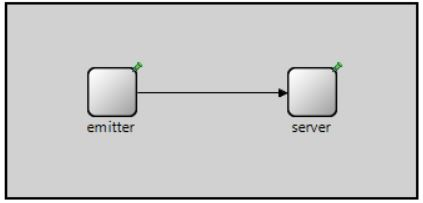
\includegraphics[width=80mm]{images/Network.JPG}
        \caption{OMNeT++ model}
        \label{fig:Omnet_model}
    \end{figure}
    \newline
    Our network is composed by two simple modules, an emitter that sends jobs and a server that receives them, puts them in a queue and serves them. The emitter has two factors, the inter-arrival time and the service-time, while the server has only one factor, the vacation period. For each one of them we created a different Random Number Generator from the .ini file having different seed that also changes depending on the repetition id.
    \lstinputlisting[language=Octave]{omnet++_code/simpleEmitter_ned.txt}
    \subsection{Emitter}
        A simple module that sends jobs to the server. 
        
        \subsubsection{Emitter.ned}
        Its parameters are:
        \begin{itemize}
            \item 
            \begin{verbatim}constant:\end{verbatim}
            a boolean that specifies if we are using constant values or exponential distributions;
            \item 
            \begin{verbatim}interarrival_time:\end{verbatim}
            it is the value of inter-arrival times in case we are using constant values, otherwise it is the mean of the exponential distribution;
            \item 
            \begin{verbatim}requested_service_time:\end{verbatim}
            it represents either the constant service time of each job or the mean of the exponential distribution of service times.
        \end{itemize}
        It has only one output gate.
        \lstinputlisting[language=Octave]{omnet++_code/Emitter_ned.txt}
        
        \subsubsection{Emitter.h}
        \lstinputlisting[language=Octave]{omnet++_code/Emitter_h.txt}
        
        \newpage
        \subsubsection{Emitter.cc}
        When the emitter is initialized, the function \textit{initialize()} obtains the values of arrival time and service time, then it creates the first job that it wants to send and sets its service time. In the end it schedules a message after a period equal to \textit{arrival\_time}.
        \newline
        Then, when a self message is received, it creates a new message, sets the values and schedules a new message after a period equal to \textit{arrival\_time}. This is done by the function \textit{handleMessage(cMessage *msg)}.
        \lstinputlisting[language=Octave]{omnet++_code/Emitter_cc.txt}
    
    \subsection{Server}
    A simple module that receives jobs through its input gate, queues them and serves them as described in paragraph 1.
    
        \subsubsection{Server.ned}
        For what concerns its structure, the server has the following parameters:
         \begin{itemize}
            \item 
            \begin{verbatim}constant:\end{verbatim}
            as before, it specifies if we are using constant values or exponential distributions;
            \item
            \begin{verbatim}vacation_time:\end{verbatim}
            in case we are using constant values it is the duration of the vacation, otherwise it corresponds to the mean of the exponential distribution;
            \item
            \begin{verbatim}turn_time:\end{verbatim}
            it is a constant value representing the duration of the turn.
        \end{itemize}
        We have two more parameters that allow us to define a recorder that will keep track of some statistics of the signal of the response time.
        \newline
        In the end, this module has only one input gate.
        \lstinputlisting[language=Octave]{omnet++_code/Server_ned.txt}
        
        \newpage
        
        \subsubsection{Server.h}
        \lstinputlisting[language=Octave]{omnet++_code/Server_h.txt}
        
        \newpage
        
        \subsubsection{Server.cc}
        When the \textit{initialize()} is called, the server instantiates his parameters and then he immediately starts a vacation, since when the server begins his service the queue will be empty. After the vacation is ended he starts his standard workflow. When it receives a Job from the emitter, it always adds it to the queue since the Server will be either in vacation or already serving a Job. The queue is composed by a list of structures keeping information about the \textit{arrival time} and the \textit{required service time}. 
        In order to compute the \textit{response time}, every time a Job is served we check the departure time of the Job.
        \lstinputlisting[language=Octave]{omnet++_code/Server_cc.txt}
        
    \subsection{Job}
    We extended the cMessage by adding a string value which contains the requested service time for that specific Job. We chose the string so that we can convert the requested service time, that is a simtime\_t, to a string and back again to it's original type.
        \subsubsection{Job.msg}
        \lstinputlisting[language=Octave]{omnet++_code/Job_msg.txt}
        
\newpage

\section{Queueing theory model}

    We studied a simplified version of the system using queueing theory in order to check if the OMNeT++ model we designed was working appropriately.
    
    To perform queueing theory modeling we considered the scenario with \textbf{exponential arrival rates}, \textbf{exponential service rates} and \textbf{no server's vacations}.
    
    \subsection{Simplifications}
    
        To model the system with queueing theory we have neglected the vacations of the server. With this simplification, turns does not make sense anymore because even if we have to calculate a deficit because we have a turn that can't serve a specific job, since we have no vacation, the time required to get a turn time big enough to serve that job is null, so it's exactly like an M/M/1 system.
        \newline
        With this simplification the system can be modeled as an \textbf{M/M/1 system} with:
        \begin{itemize}
            \item $E[t_s] = {1 \over \mu}$ = mean service time
        \end{itemize}


    \begin{figure}[ht!]
        \centering
        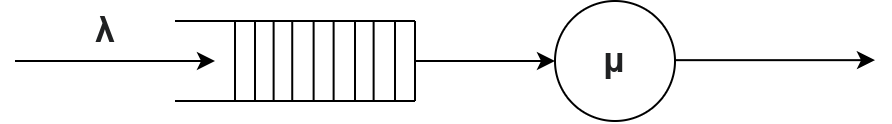
\includegraphics[scale=0.2]{./images/system_queueing_theory}
        \caption{Simple model of the system for queueing theory}
        \label{fig:system_queueing_theory}
    \end{figure}
    
    \begin{figure}[ht!]
        \centering
        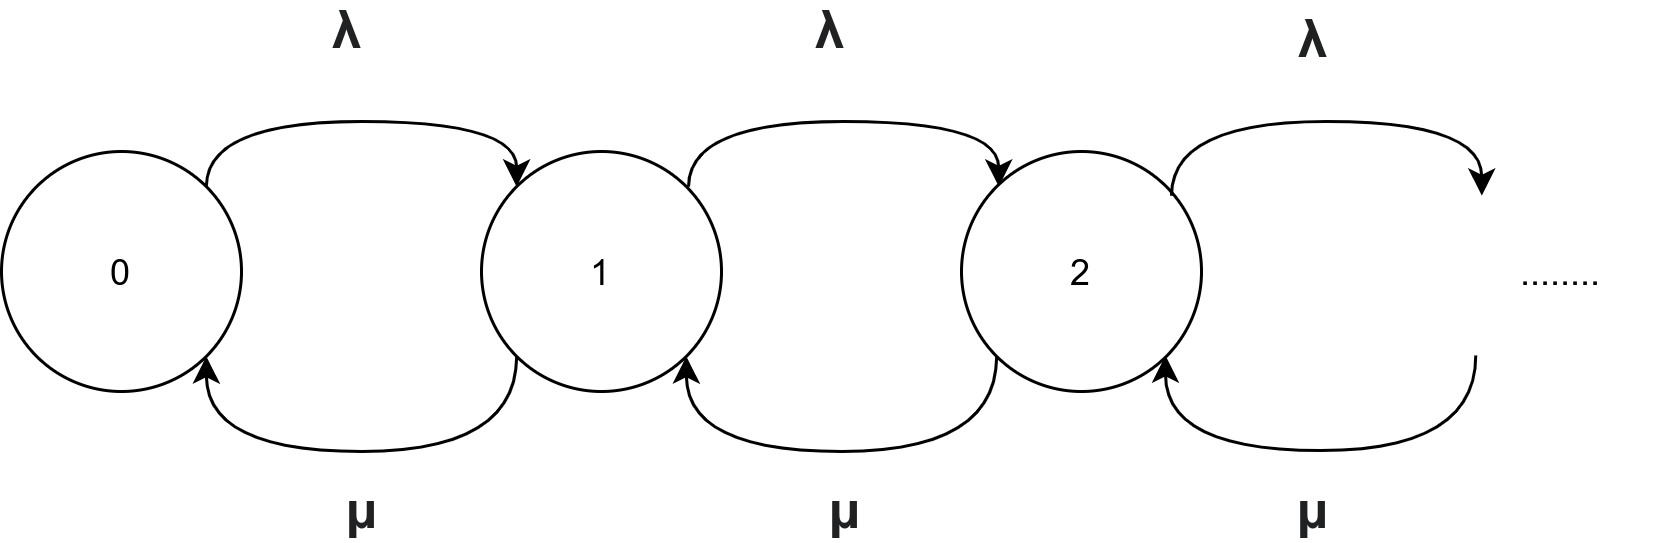
\includegraphics[scale=0.18]{./images/CTMC_no_vacations}
        \caption{CTMC considering no server's vacations}
        \label{fig:CTMC_no_vacations}
    \end{figure}
    
    In state denoted as $i$ there are exactly $i$ jobs in the system.

    \subsection{Computing the SS probabilities}
    
        \subsubsection{Local equilibrium equations}
            
            \[
            \left\{
                \begin{array}{rcrc}
                    p_0 \cdot \lambda = p_1 \cdot \mu & n=0 \\
                    p_j \cdot \lambda  = p_{j+1} \cdot \mu & n \ge 1
                \end{array}
            \right.
            \]
        
            From the \textit{local equilibrium equations} can be obtained $p_n$ as a function of $p_0$ as it follows:
            
            \[p_n=\left({\lambda \over \mu}\right)^n \cdot p_0\]
        
        \subsubsection{Normalization condition}
        
            We can compute the \textit{normalization condition} as:
            
            \[
            p_0\cdot \left [\sum_{j=0}^{+\infty}({\lambda \over \mu})^n \right]=1
            \]
        
        \subsubsection{Solving the SS system}
        
            The system composed by the local equilibrium equations and the normalization condition can be solved and the unique solution for the steady-state probabilities is:
                \[
                \left\{
                    \begin{array}{rcrc}
                        p_0 = 1-{\lambda \over \mu} \\
                        p_n={\lambda^n \over \mu^n} \cdot p_0
                    \end{array}
                \right.
                \]
            
            The \textbf{stability condition} for the system is $\lambda < \mu$
            
            The \textbf{Utilization} of the system is $\rho = {\lambda \over \mu}$
    
    \subsection{Checking the PASTA condition}
    
        The system is PASTA because $\lambda_n = \lambda$ $\forall n$.
    
    \subsection {Little's Law and Mean Performance Indexes}
    
        We can apply Little's Law in order to compute mean performance indexes and we can apply M/M/1's formulas.
        
        \begin{itemize}
        
            \item $E[R] = {E[N] \over \overline{\lambda}} = {1\over \mu -\lambda}$
            
            \item $E[N] = {\rho \over 1-\rho } = { {\lambda \over \mu} \over {1-{\lambda \over \mu}}}$
        \end{itemize}

\newpage 

\section{Validation}

    In order to validate our OMNeT++ model, we used a simplified version of the system where the server doesn't go on vacation. In this way we compared the results for the mean response time obtained with simulation against those obtained using the model designed with queuing theory. In particular we noticed that the mean response time $E[R]$ of the simulations, ran with \textbf{vacations = 0ms} and \textbf{exponential arrival rates} and \textbf{exponential service times}, was almost equal to ${1 \over \mu - \lambda}$.
    Making the comparisons of the results we noticed that the system was working as we expected to be working so we can state that our simulation model is valid.\\
    
    To perform the validation of the OMNeT++ model we changed in the code the Vacation duration to $0ms$ so the Server will still go on vacation and it will still handle turns. We had to modify some parts of Server.cc because there were some problems related to putting $Vacations=0ms$: if the Server goes on vacation when there are no jobs in the queue, it will wake up after $0ms$ and will find the queue empty again and will schedule another vacation of $0ms$, in this way the Server will fall in an infinite loop because the simulated time cannot advance and an arriving job has no time to queue up since its related event won't be handled by the Server. To solve this issue we used a boolean variable \textit{working}: \textit{working = true} if the server is handling a job, otherwise \textit{working = false}. When the server receives a job, if \textit{working = true} then the arriving jobs is putted in the queue, otherwise the server starts its service and sets \textit{working = true}. 

    When the server finishes to serve a job and the turn isn't finished yet, it checks whether there are any another jobs in the queue or not. If there aren't any other jobs, it sets \textit{working=false} and goes idle instead of going on vacation, in this way we avoided the infinite loop. In the end it will re-start its service whenever a new job arrives.
    Otherwise, if there are jobs in the queue, it evaluates the requested service time of the new job and if it is larger than the remaining time goes on vacation in order to build a turn large enough. Since vacations are 0ms long, it immediately builds a turn large enough and starts the service. This means that the system works as an M/M/1.\\
    
    The Server is initialized with \textbf{working=false} and it starts on an idle state.

    \newpage
    
    \lstinputlisting[language=Octave]{omnet++_code/ServerValidation_cc.txt}
    
\newpage

\section{Constant case}
    
    We started analyzing the system with constant values for inter-arrival times, service times and vacation period. We tested it in limit cases and observed that, for different values of Q the system behaves in a different way. In particular, \textbf{the smaller the value of the turn, the higher needs to be the inter-arrival time, maintaining all the other values equal}. For instance, let's analyze the case for $Q =\frac{S_t}{2}$: since the turn time is half the time required for a job to be served, the system will have to go on vacation two times to handle the request of the job, one in order to build a turn big enough, one after the job is served. Knowing that, we can easily state that every time the system will have to take two vacations and one service time for each job that arrives.
    \newline
    In the end we wrote a stability condition for our system: \[Inter\-arrival\_time \ge Vacation \cdot \frac{Service\_time}{Q} + Service\_time \]
    To prove our statement we simply changed values here and there and plotted the results.
    Note that, if $Q \rightarrow \infty$, then the first addendum of the above formula goes to 0, meaning that our system behaves like an M/M/1 system, which is the same as stating that our server doesn't go on vacation.

    \subsection{Testing the hypothesis}
        Here we report some plots where we have considered these two cases for different values of Q(1/10, 1 and 10 service times):
        \begin{enumerate}
            \item $Inter\-arrival\_time = Vacation \cdot \frac{Service\_time}{Q} + Service\_time$     \crule[red]{3mm}{3mm}
            \item $Inter\-arrival\_time < Vacation \cdot \frac{Service\_time}{Q} + Service\_time$
            \crule[blue]{3mm}{3mm}
        \end{enumerate}
        
        \begin{paragraph}
        \centering
            \centering \paragraph{Q=3ms} \hfill \\
            \begin{figure}[htbp]
                \centering
                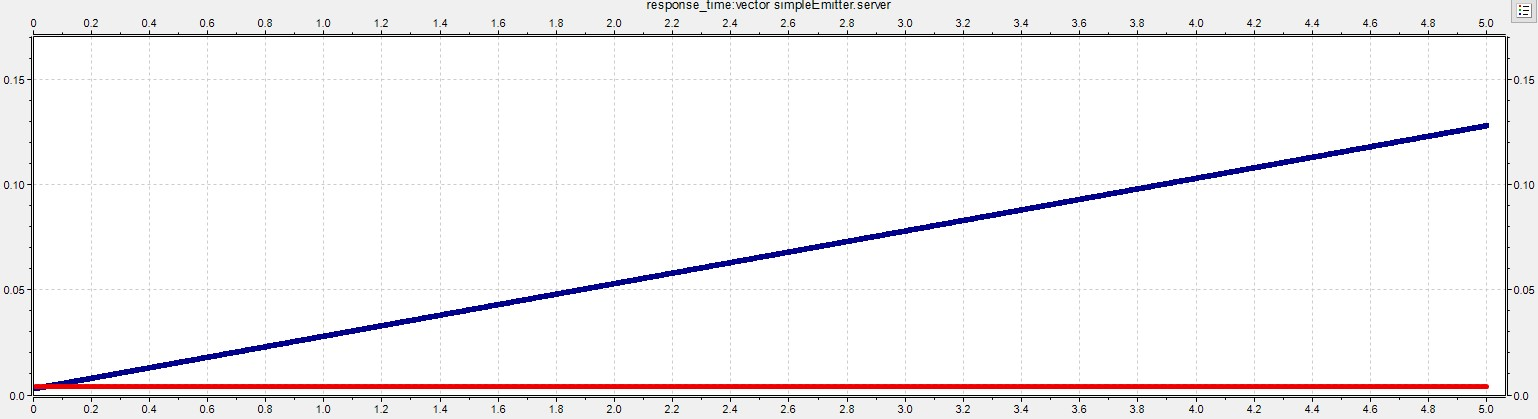
\includegraphics[scale=0.3]{./images/constant_case/3ms.jpg}
                \caption{Interarrival= {\color{blue}{3,9ms}} e {\color{red}{4ms}}; Service time=3ms; Vacation=1ms.}
                \label{fig:constant_3ms}
            \end{figure}
        \end{paragraph}
        
        \begin{paragraph}
        \centering
            \centering \paragraph{Q=30ms} \hfill \\
            \begin{figure}[htbp]
                \centering
                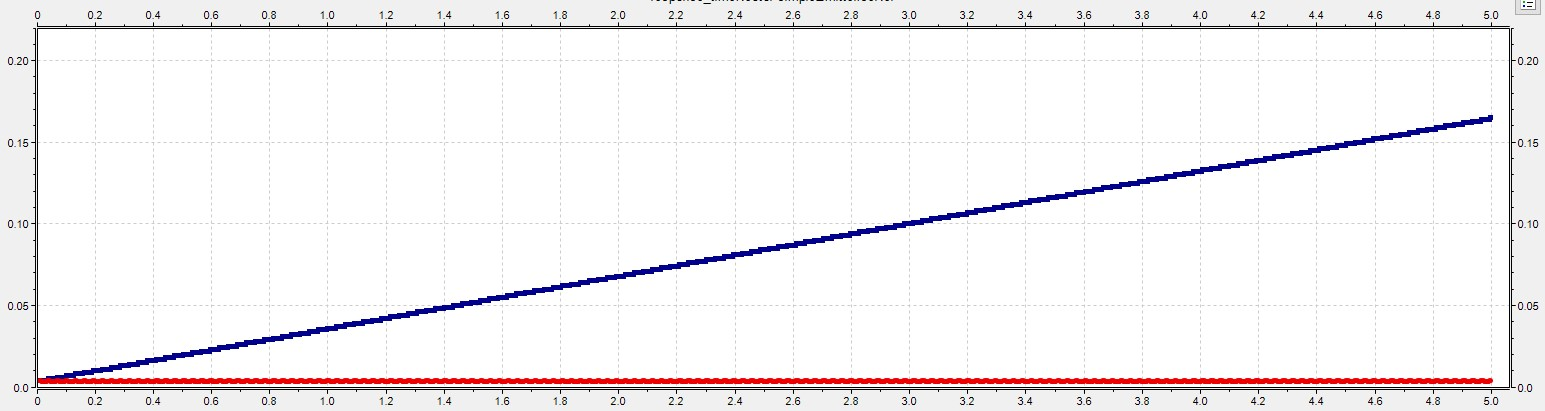
\includegraphics[scale=0.3]{./images/constant_case/30ms.jpg}
                \caption{Interarrival= {\color{blue}{3ms}} e {\color{red}{3,1ms}}; Service time=3ms; Vacation=1ms.}
                \label{fig:constant_30ms}
            \end{figure}
        \end{paragraph}
        
        \begin{paragraph}
        \centering
            \centering \paragraph{Q=0,3ms} \hfill \\
            \begin{figure}[htbp]
                \centering
                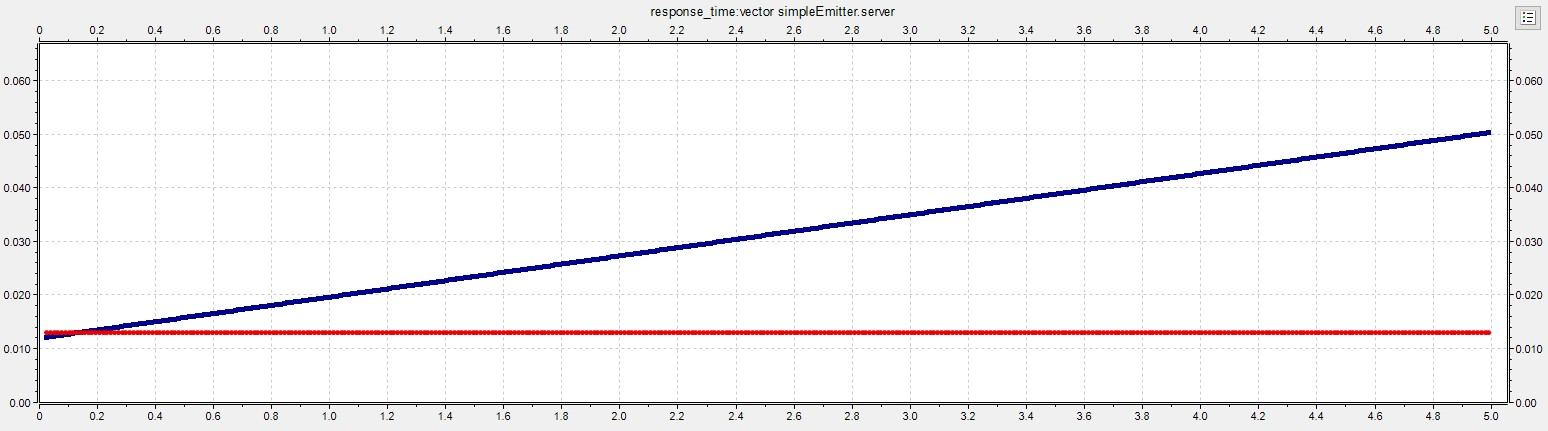
\includegraphics[scale=0.3]{./images/constant_case/03ms.jpg}
                \caption{Interarrival= {\color{blue}{12,9ms}} e {\color{red}{13ms}}; Service time=3ms; Vacation=1ms.}
                \label{fig:constant_03ms}
            \end{figure}
        \end{paragraph}

\newpage

\section{Exponential case}

    From now on we will use, for simplicity, $\mu$ for the Mean Service time; $\delta$ for the Mean Vacation period; $\lambda$ for the Mean Inter-arrival time.

    \subsection{Tuning of the parameters for the simulations}

        We performed the tuning of the parameters for the simulations for $5$ different scenarios because we noticed that it was necessary to have different values for the parameters depending on the ratio between $Q$ and $S_t$ $(\frac{1}{10}, \frac{1}{2}, 1, 5, 10)$ in order to make the system stable.\\ 
        
        The min value and max value for \textbf{inter-arrival time} have been estimated using some information found on data-sheets.
        
        The min and max values for the service time and the vacations have been estimated taking in consideration that should be:
        \[\frac{service\_time}{Q}*vacations + service\_time < inter\_arrivals\]
        
        Then, for each case we have made different trials and we have selected a range of values that made the system stable in both the best and worst scenarios, but still had some interesting values, meaning that it does involve queuing and may have peaks of response time depending on the variability of the factors.
        We also decided to variate only the values of the inter-arrival time, maintaining the same two couple of values for vacations and service time because in this way we can easily state that with big values of $Q$ we can use lower inter-arrival times making the system faster and for small values of $Q$ we can make it extremely slower and sensible to variability. 
        
        \subsubsection{Scenario $Q = S_t$}
        
            \begin{table}[htbp!]
                \centering 
                \begin{tabular}{|l|c|c|}
                    \hline
                    \ & Min & Max \\
                    \hline
                    inter-arrival time & $16ms$ & $20ms$ \\
                    \hline
                    service time & $3ms$ & $7ms$ \\
                    \hline
                    vacation & $1ms$ & $5ms$ \\
                    \hline
                \end{tabular}
                \caption{min and max for the mean value of the parameters in the case $Q = S_t$} 
            \end{table}
            
        \subsubsection{Scenario $Q = 10S_t$}
        
            \begin{table}[htbp!]
                \centering 
                \begin{tabular}{|l|c|c|}
                    \hline
                    \ & Min & Max \\
                    \hline
                    inter-arrival time & $8ms$ & $12ms$ \\
                    \hline
                    service time & $3ms$ & $7ms$ \\
                    \hline
                    vacation & $1ms$ & $5ms$ \\
                    \hline
                \end{tabular}
                \caption{min and max for the mean value of the parameters in the case $Q = 10S_t$} 
            \end{table}
        
        \newpage
        
        \subsubsection{Scenario $Q = \frac{1}{10} S_t$}
             \begin{table}[htbp!]
                \centering 
                \begin{tabular}{|l|c|c|}
                    \hline
                    \ & Min & Max \\
                    \hline
                    inter-arrival time & $77ms$ & $81ms$ \\
                    \hline
                    service time & $3ms$ & $7ms$ \\
                    \hline
                    vacation & $1ms$ & $5ms$ \\
                    \hline
                \end{tabular}
                \caption{min and max for the mean value of the parameters in the case $Q = \frac{1}{10} S_t$} 
            \end{table}
        
         \subsubsection{Scenario $Q = \frac{1}{2} S_t$}
             \begin{table}[htbp!]
                \centering 
                \begin{tabular}{|l|c|c|}
                    \hline
                    \ & Min & Max \\
                    \hline
                    inter-arrival time & $22ms$ & $26ms$ \\
                    \hline
                    service time & $3ms$ & $7ms$ \\
                    \hline
                    vacation & $1ms$ & $5ms$ \\
                    \hline
                \end{tabular}
                \caption{min and max for the mean value of the parameters in the case $Q = \frac{1}{2} S_t$} 
            \end{table}
            
        \subsubsection{Scenario $Q = 5S_t$}
             \begin{table}[htbp!]
                \centering 
                \begin{tabular}{|l|c|c|}
                    \hline
                    \ & Min & Max \\
                    \hline
                    inter-arrival time & $10ms$ & $14ms$ \\
                    \hline
                    service time & $3ms$ & $7ms$ \\
                    \hline
                    vacation & $1ms$ & $5ms$ \\
                    \hline
                \end{tabular}
                \caption{min and max for the mean value of the parameters in the case $Q = 5S_t$} 
            \end{table}
    
    \newpage
    
    \subsection{Estimation of the warm-up period}
    
        To estimate the duration of the warm-up period, we did $40$ $simulations$ ($5$ independent repetitions of $8$ different scenarios).\\
        
        The warm-up period was estimated taking into consideration all the different cases shown above. 
        Here we report two plots of the sliding window average in two of the cases in which $Q = S_t$ and $Q = 10S_t$.
        
        \begin{figure}[ht!]
            \centering
            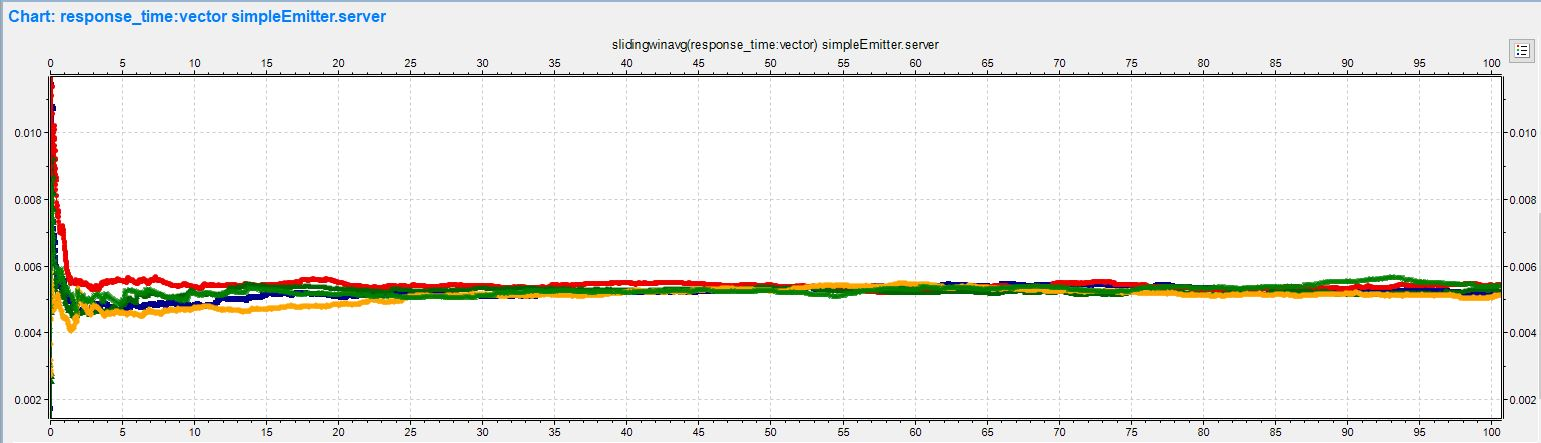
\includegraphics[scale=0.3]{./images/sliding_window_averages/case5ms.JPG}
            \caption{Sliding window average of the response time (case $Q = S_t$)}
            \label{fig:sliding_avg_case5ms}
        \end{figure}
        
        \begin{figure}[ht!]
            \centering
            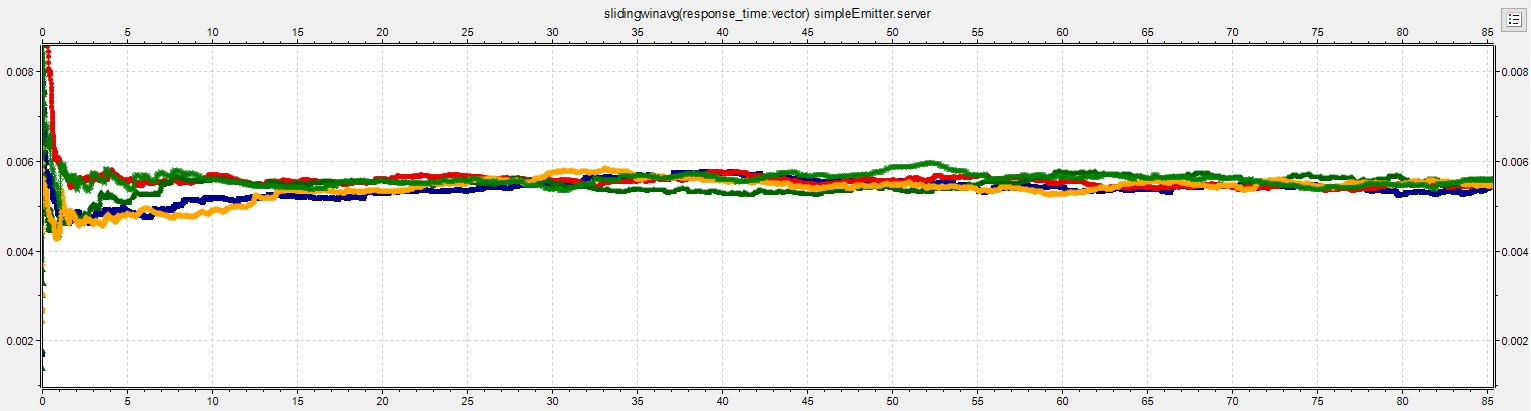
\includegraphics[scale=0.3]{./images/sliding_window_averages/case50ms.jpg}
            \caption{Sliding window average of the response time (case $Q = 10S_t$)}
            \label{fig:sliding_avg_case50ms}
        \end{figure}
        
        As we can notice from figure \ref{fig:sliding_avg_case5ms} and \ref{fig:sliding_avg_case50ms}, the duration of the warm-up period can be estimated at $3s$.
        
    \newpage
    
    \subsection{$2^k r$ factorial analysis}
    
        In order to understand which factor affects the most the mean response time, we performed the $2^k r$ factorial analysis with $3$ factors (inter-arrivals $\lambda$, services $\mu$ and vacations $\delta$), $5$ repetitions and $Q= \left\{ \frac{1}{10} S_t, \frac{1}{2}S_t, S_t, 5S_t, 10S_t \right\}$, for $Q$ we chose to perform the $2^k r$ factorial analysis both in the case with $Q=S_t$ (Variable Q case) and $Q=\frac{S_{t_{Min}} + S_{t_{Max}}}{2}$ (Constant Q case). For the cases $Q = \frac{1}{2}S_t$ and $Q = 5S_t$ we only analyzed the variable Q case.\\
        
        With the factorial analysis we noticed that the \textit{Constant Q case} brings out some issues. In fact, let's assume we have Q = 5ms, and the service time has a min value of 3ms and a max of 7ms. It's easy to see that for the case in which the service time is lower, the system will be faster and less sensible to variations, since even if we end up having a big job, it will probably be served within the turn. That does the exact opposite for the case in which we have the highest service time, this time the job will almost every time make the system go on vacation once in order to be served. For bigger values of Q this issue is negligible, since we will have Q = 50ms, and the worst case for the service time is 7ms, so we will end up serving, on average, 7 jobs before the vacation, instead of 10, while for a service time of 3ms we will have one vacation every 16 jobs, so for both cases we will add, or remove, just a few more vacation, so we won't increment, or decrease, a lot the mean response time of the system. If we check this for the system with Q = 0,5ms then for the service time at 3ms we will need 6 vacations in order to serve one job, if instead the service time is at 7ms, we'll end up taking 14 vacations for each job, meaning that we will change a lot the value of the mean response time. This leads to an interesting consideration about the system itself: \textbf{the smaller the value of $\frac{Q}{S_t}$ is, the more the system will be sensible to small variations of Q.} \\
        
        For the simulations used to collect the data needed to perform the $2^k r$ factorial analysis we used the values found with the tuning for the factors.\\
        
        For what concerns testing the hypothesis, we tested that residuals were normally distributed using a normal QQ plot, while we created a scatterplot of the residuals vs. the predicted response to test constant std. We also wanted to test IIDness using a scatterplot of the residuals vs the observation number, but we didn't know the sequence of observations so we assumed there was no bias.
    
        \newpage 
        \subsubsection{Case $Q = S_t$}
                
            \paragraph{Results} \hfill \\
                As we can see from the table of the variations, in this case the factors that matter the most are \textit{vacations}, \textit{service times} and the \textit{interplay of vacations and service times}.
                This makes sense since the system, on average, will serve a job and then start a vacation.
                
                \begin{table}[htbp]
                    \centering 
                    \begin{tabular}{|c|c|c|c|c|c|c|c|}
                        \hline
                        \multicolumn{8}{|c|}{\bf Percentage of variation of the factors and the error} \\
                        \hline
                        \ $\lambda$ & $\mu$ & $\delta$ & $\lambda\mu$ & $\lambda\delta$ & $\mu\delta$ & $\lambda\mu\delta$ & $\epsilon$ \\
                        \hline
                        \ 4.48\% & 33.83\% & 48.39\% & 2.37\% & 2.59\% & 6.87\% & 1.31\% & 0.16\% \\ 
                        \hline
                    \end{tabular}
                    \label{table:variation_1}
                \end{table}
                
                \begin{table}[htbp]
                    \begin{tabular}{|c|c|c|c|c|c|c|c|}
                    
                         \hline
                         \multicolumn{8}{|c|}{\bf Confidence interval with 98\% confidence level} \\
                            
                        \hline
                        \ & $\lambda$ & $\mu$ & $\delta$ & $\lambda\mu$ & $\lambda\delta$ & $\mu\delta$ & $\lambda\mu\delta$\\
                        \hline
                        \ CI- & -0.00338 & 0.00838 & 0.01008 & -0.00252 & -0.00263 & 0.00364 & -0.00194 \\ 
                        \hline
                        \ CI+ & -0.00289 & 0.00887 & 0.01057 & -0.00203 & -0.00214 & 0.00413 & -0.00145 \\ 
                        \hline
                    \end{tabular}
                    \label{table:CI_1}
                \end{table}
            
            \paragraph{Testing hypothesis} \hfill \\
            In this case the normality assumption is verified since the QQ plot shown in Figure \ref{fig:QQplot_1} looks reasonably linear. 
            We can also assume the standard deviation as constant, despite the plot shows a certain trend (Figure \ref{fig:standardDeviation_1}). In fact, we can ignore it since the errors are one order of magnitude below the predicted response.
            
                \begin{figure}[htbp]
                    \centering
                    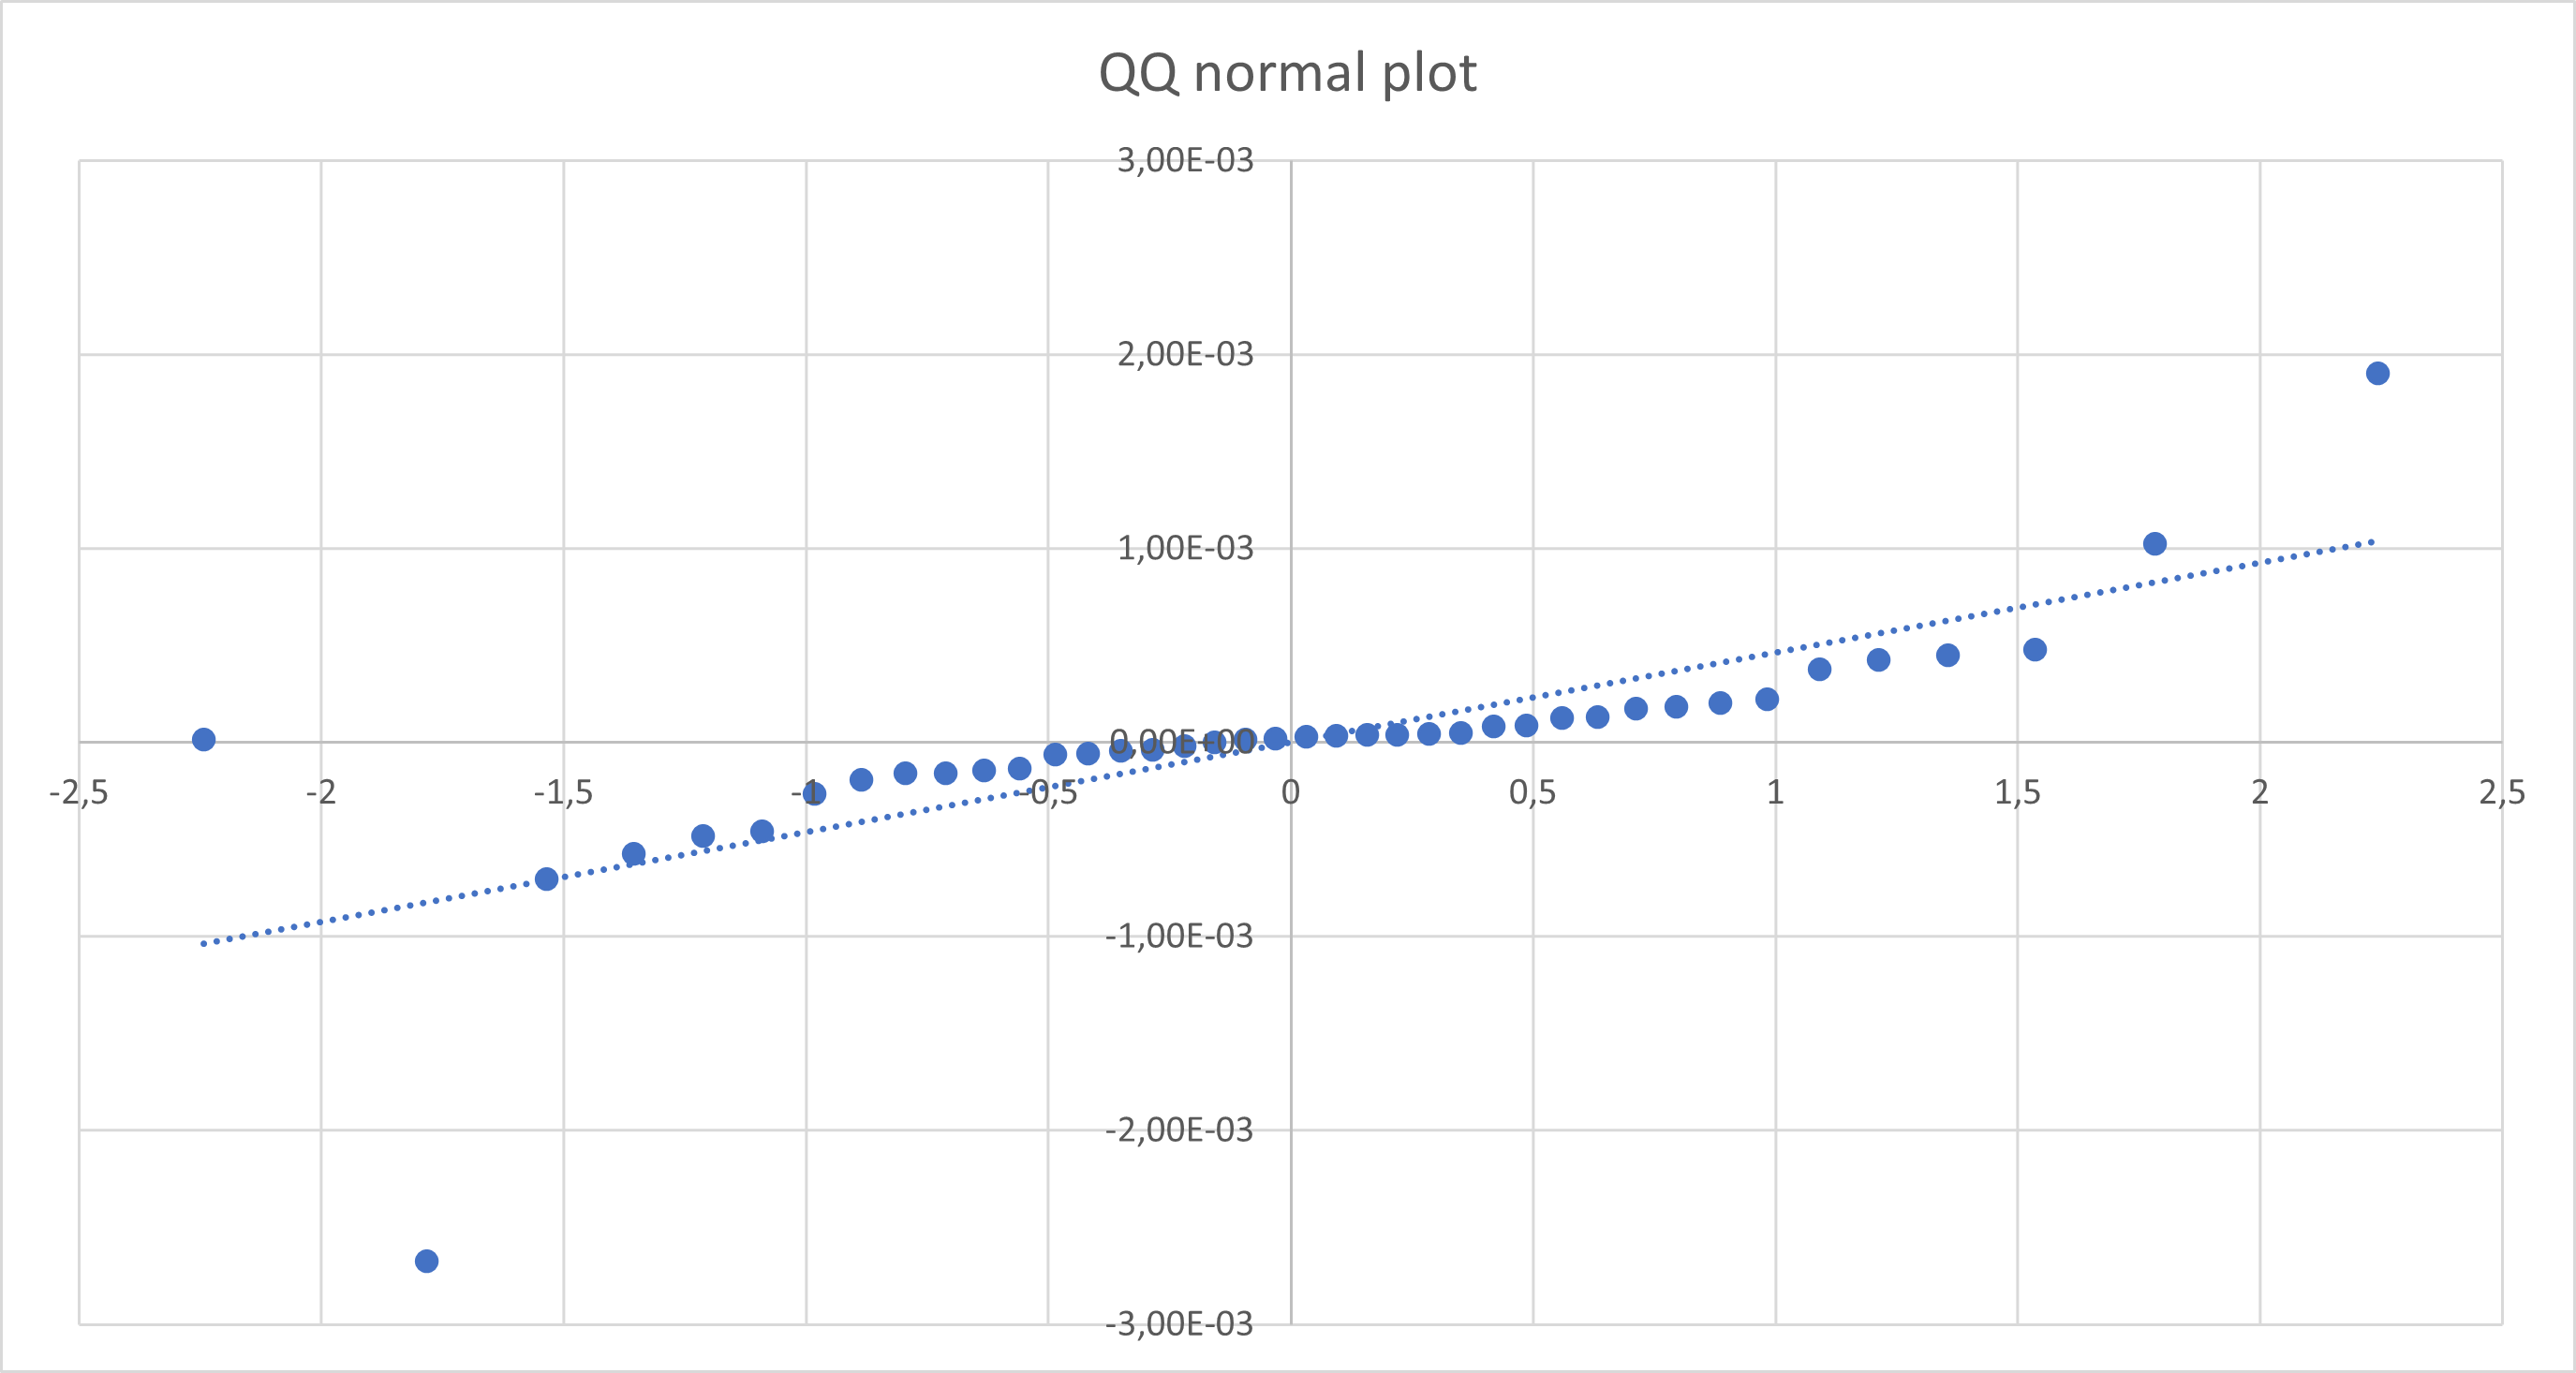
\includegraphics[scale=0.6]{images/QQplot_1.png}
                    \caption{QQ plot for $Q = S_t$}
                    \label{fig:QQplot_1}
                \end{figure}
                
                \begin{figure}[htbp]
                    \centering
                    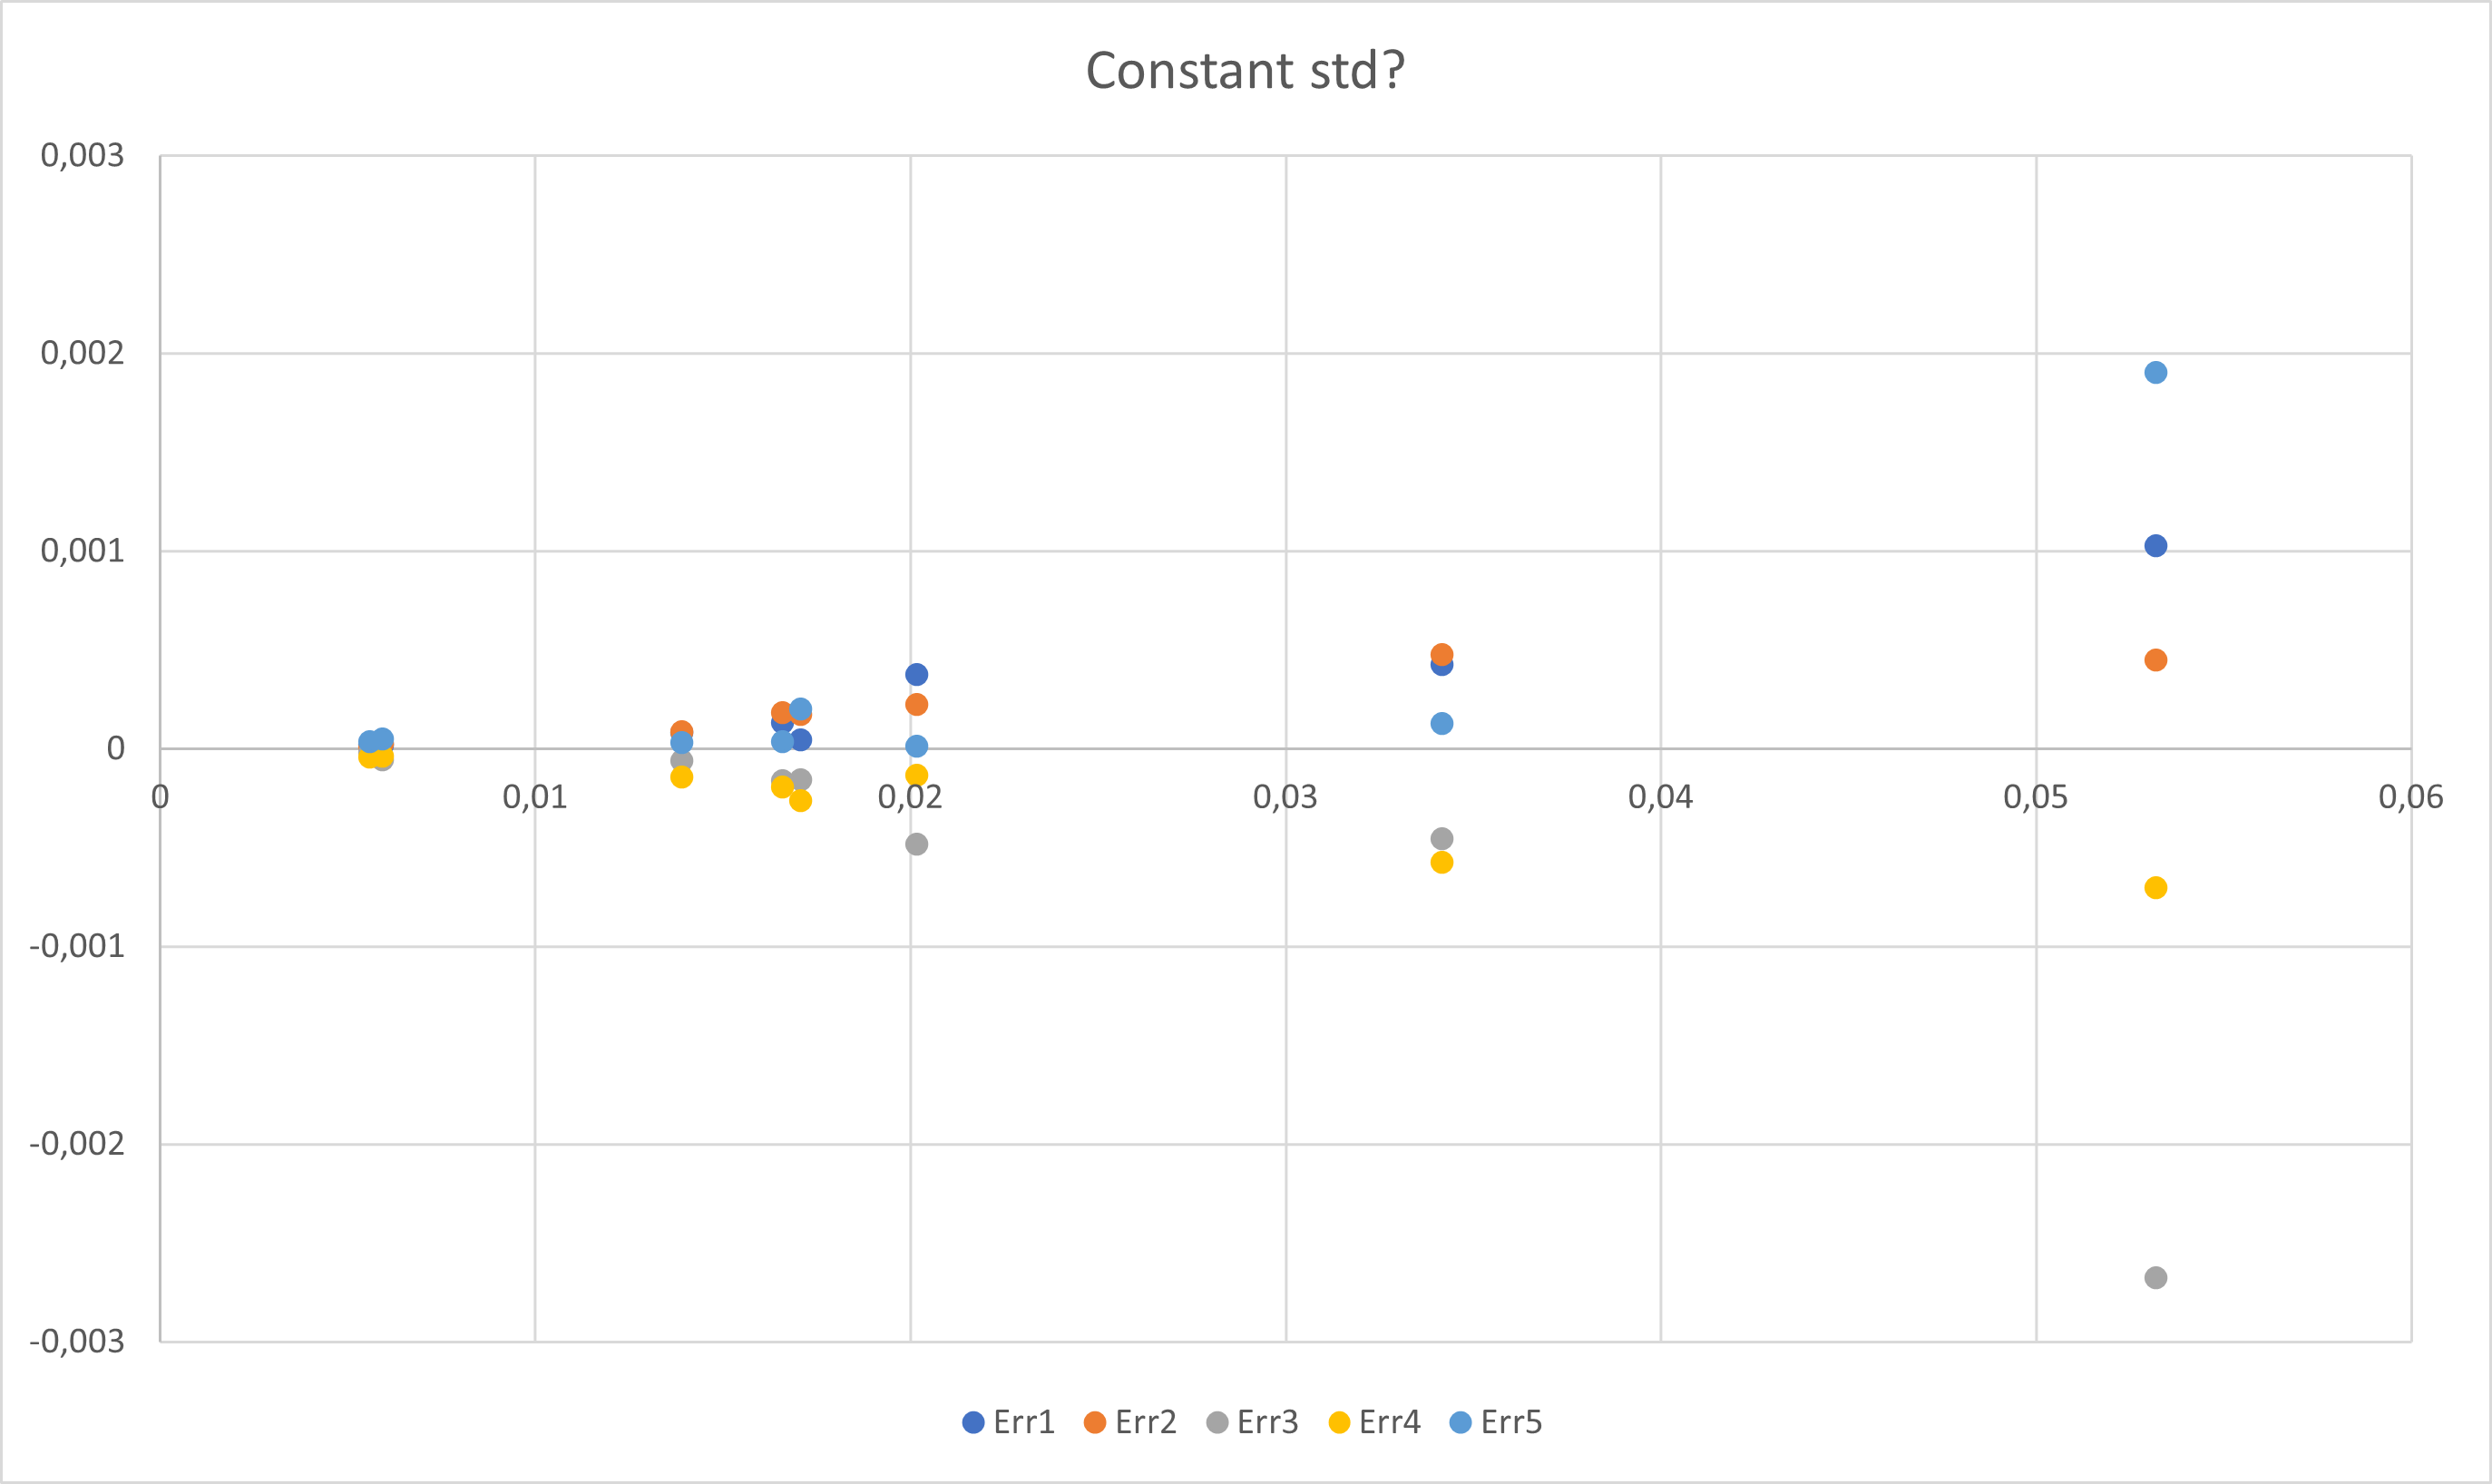
\includegraphics[scale=0.6]{images/standardDeviation_1.png}
                    \caption{Scatterplot for $Q = S_t$}
                    \label{fig:standardDeviation_1}
                \end{figure}
        
        \newpage
            \subsubsection{Case $Q = 10 S_t$}
        
                \paragraph{Results} \hfill \\
                    In the case $Q = 10 S_t$, the factors \textit{service times}, \textit{inter-arrivals} and the \textit{interplay of inter-arrivals and services} are the ones that affect the most the mean response time.
                    This is explainable by the fact that turn time is big enough to serve many jobs during a single turn, so the server rarely goes on vacation, that's why it does not really affect the performances of the system.
            +       
                    \begin{table}[htbp]
                        \centering
                        \begin{tabular}{|c|c|c|c|c|c|c|c|}
                            \hline
                            \multicolumn{8}{|c|}{\bf Percentage of variation of the factors and the error} \\
                            \hline
                            \ $\lambda$ & $\mu$ & $\delta$ & $\lambda\mu$ & $\lambda\delta$ & $\mu\delta$ & $\lambda\mu\delta$ & $\epsilon$ \\
                            \hline
                             15.96\% & 62.25\% & 5.67\% & 13.96\% & 0.61\% & 0.87\% & 0.56\% & 0.11\%\\ 
                             \hline   
                        \end{tabular}
                        \label{table:variation_10}
                    \end{table}
                
                    \begin{table}[htbp]
                        \begin{tabular}{|c|c|c|c|c|c|c|c|}
                             \hline
                             \multicolumn{8}{|c|}{\bf Confidence interval with 98\% confidence level} \\
                                
                            \hline
                            \ & $\lambda$ & $\mu$ & $\delta$ & $\lambda\mu$ & $\lambda\delta$ & $\mu\delta$ & $\lambda\mu\delta$\\
                            \hline
                            \ CI- & -0.00596 & 0.01119 & 0.00324 & -0.00558 & -0.00132 & 0.00115 & -0.00127 \\ 
                            \hline
                            \ CI+ & -0.00557 & 0.01158 & 0.00363 & -0.00519 & -0.00093 & 0.00154 & -0.00088 \\ 
                            \hline
                        \end{tabular}
                        \label{table:CI_10}
                    \end{table}
                    
                \paragraph{Testing hypothesis} \hfill \\
                    Since the QQ plot in Figure \ref{fig:QQplot_10}, except for a few points, looks approximately linear, we can state that the assumption of normality is verified.
                    
                    \begin{figure}[htbp]
                        \centering
                        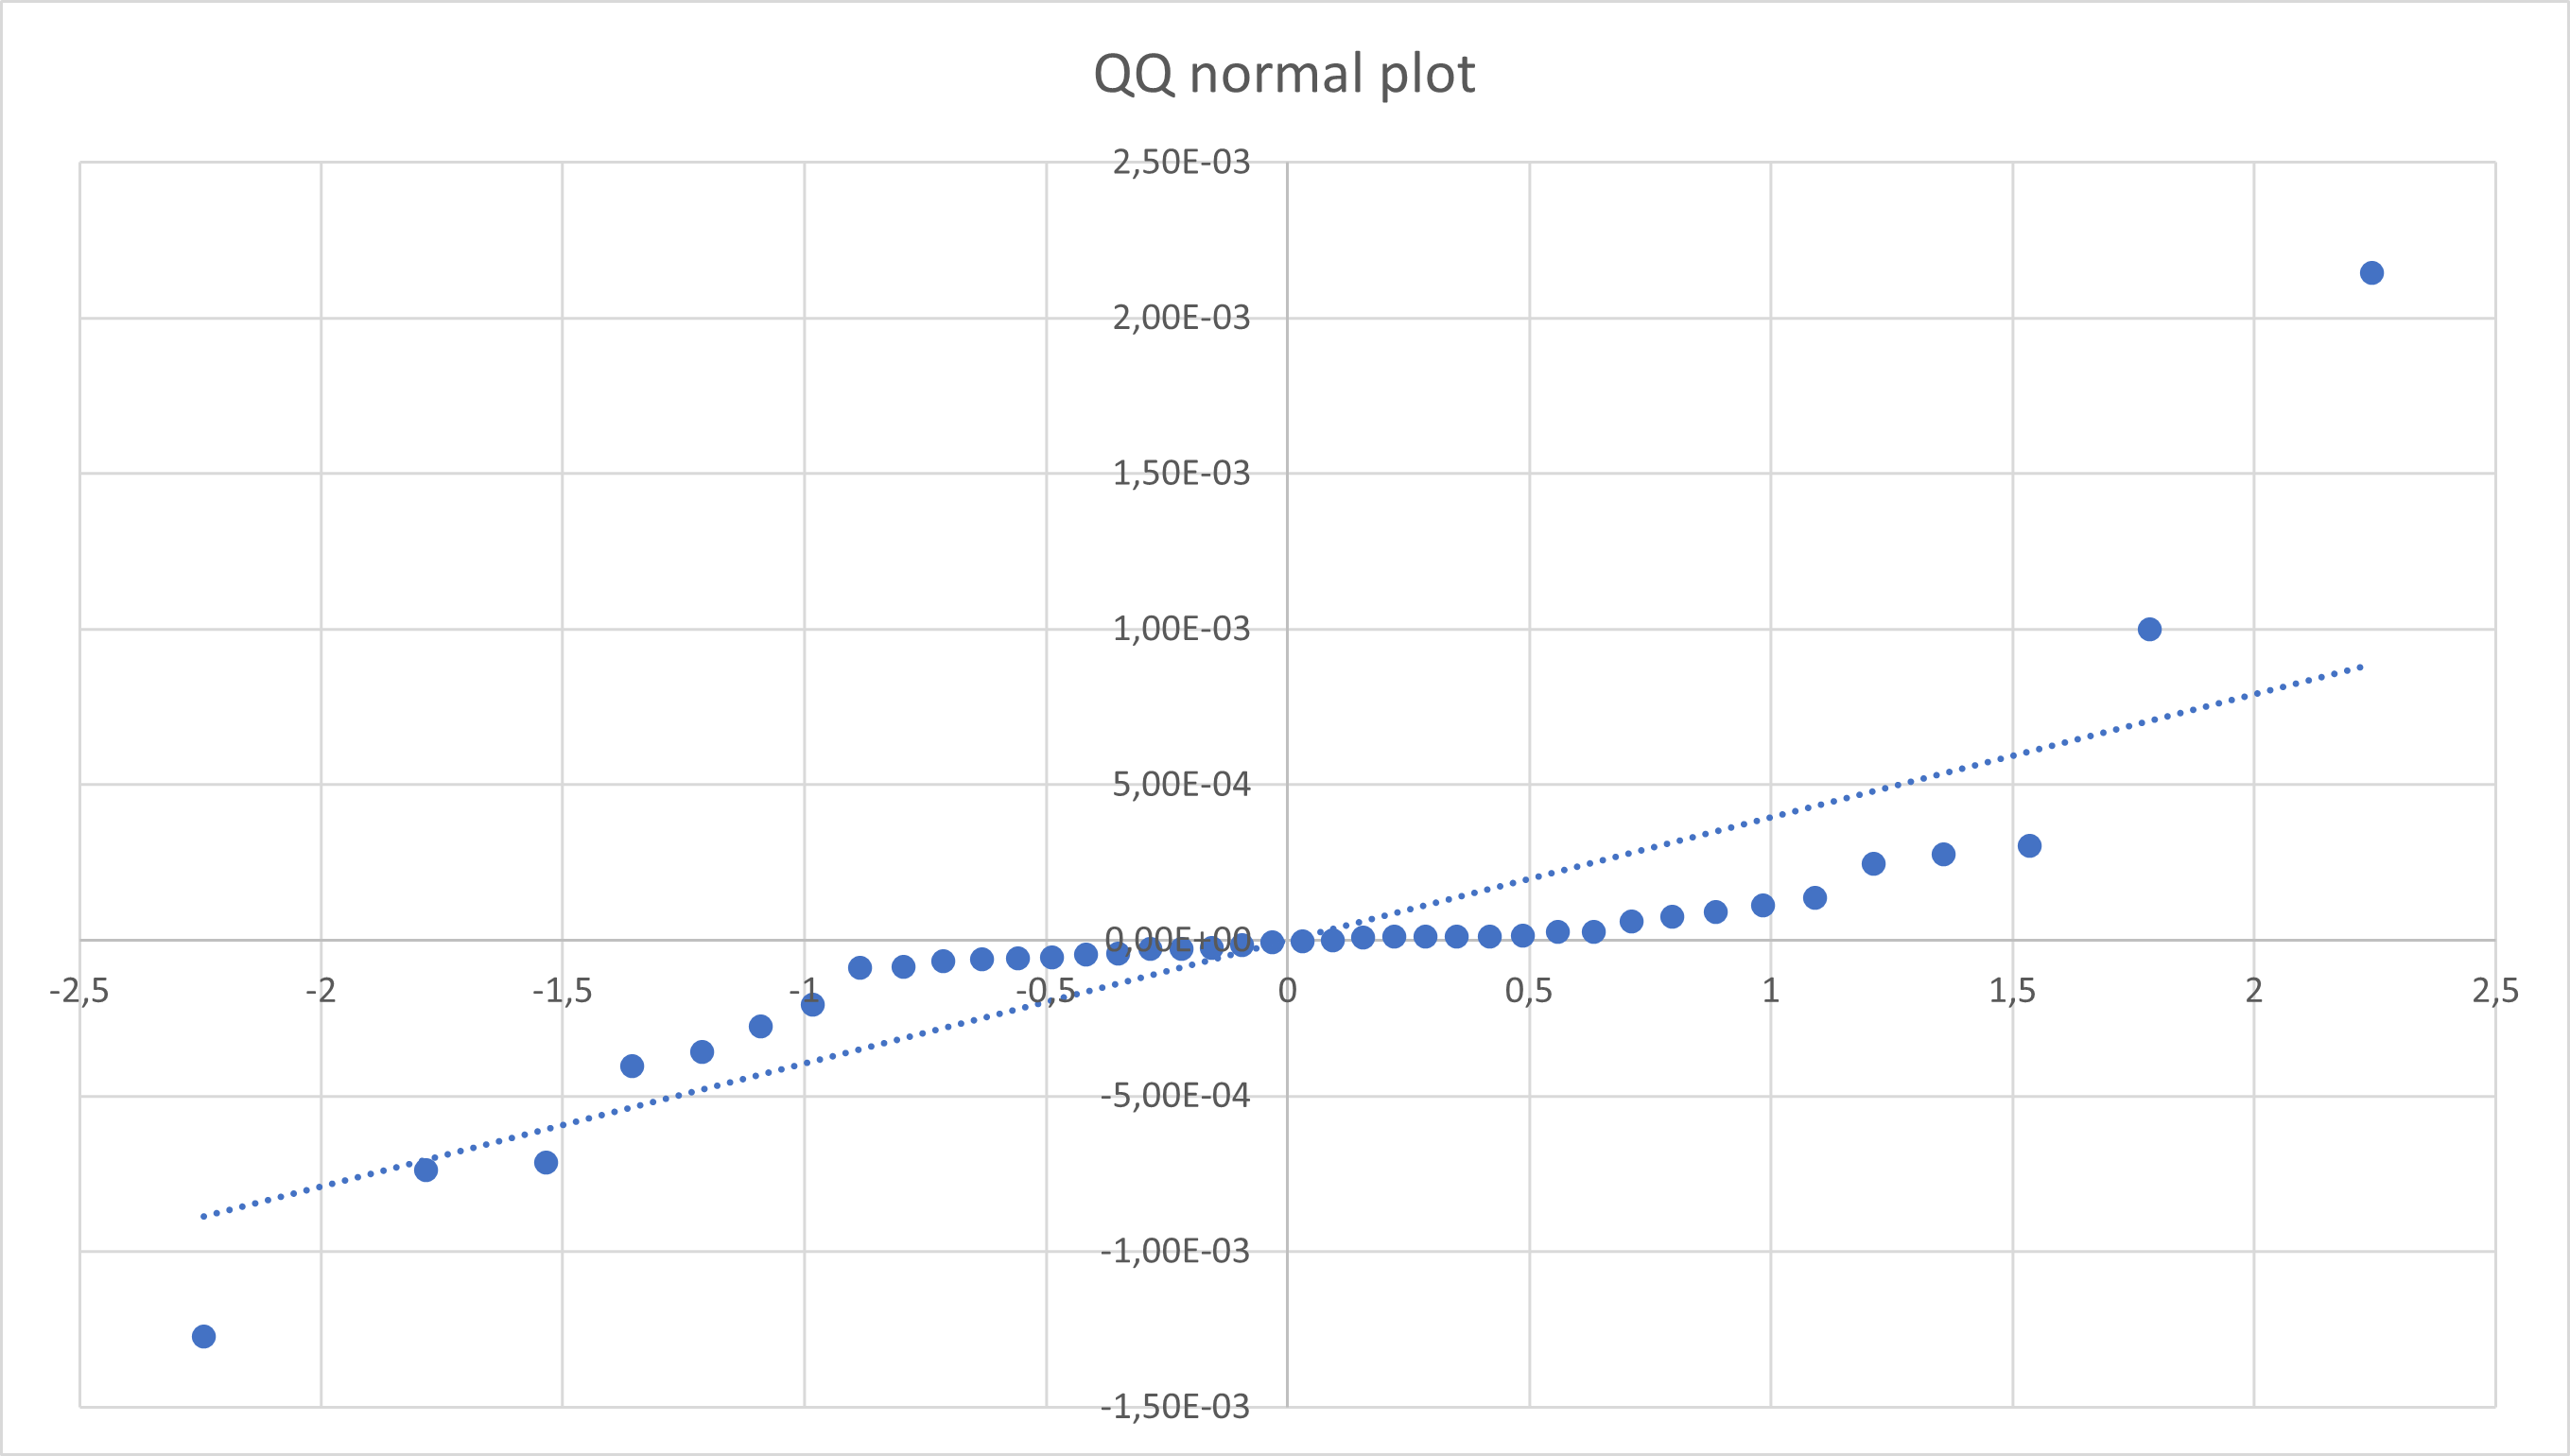
\includegraphics[scale=0.6]{images/QQplot_10.png}
                        \caption{QQ plot for $Q = 10 S_t$}
                        \label{fig:QQplot_10}
                    \end{figure}
                    
                    From Figure \ref{fig:standardDeviation_10} we can notice that the standard deviation doesn't look constant but if we pay attention to the axis' scales, we can see that the $y$s are significantly smaller than the $x$s, as a consequence we ignore the trend and we consider the standard deviation to be approximately constant.
                    
                    \begin{figure}[htbp]
                        \centering
                        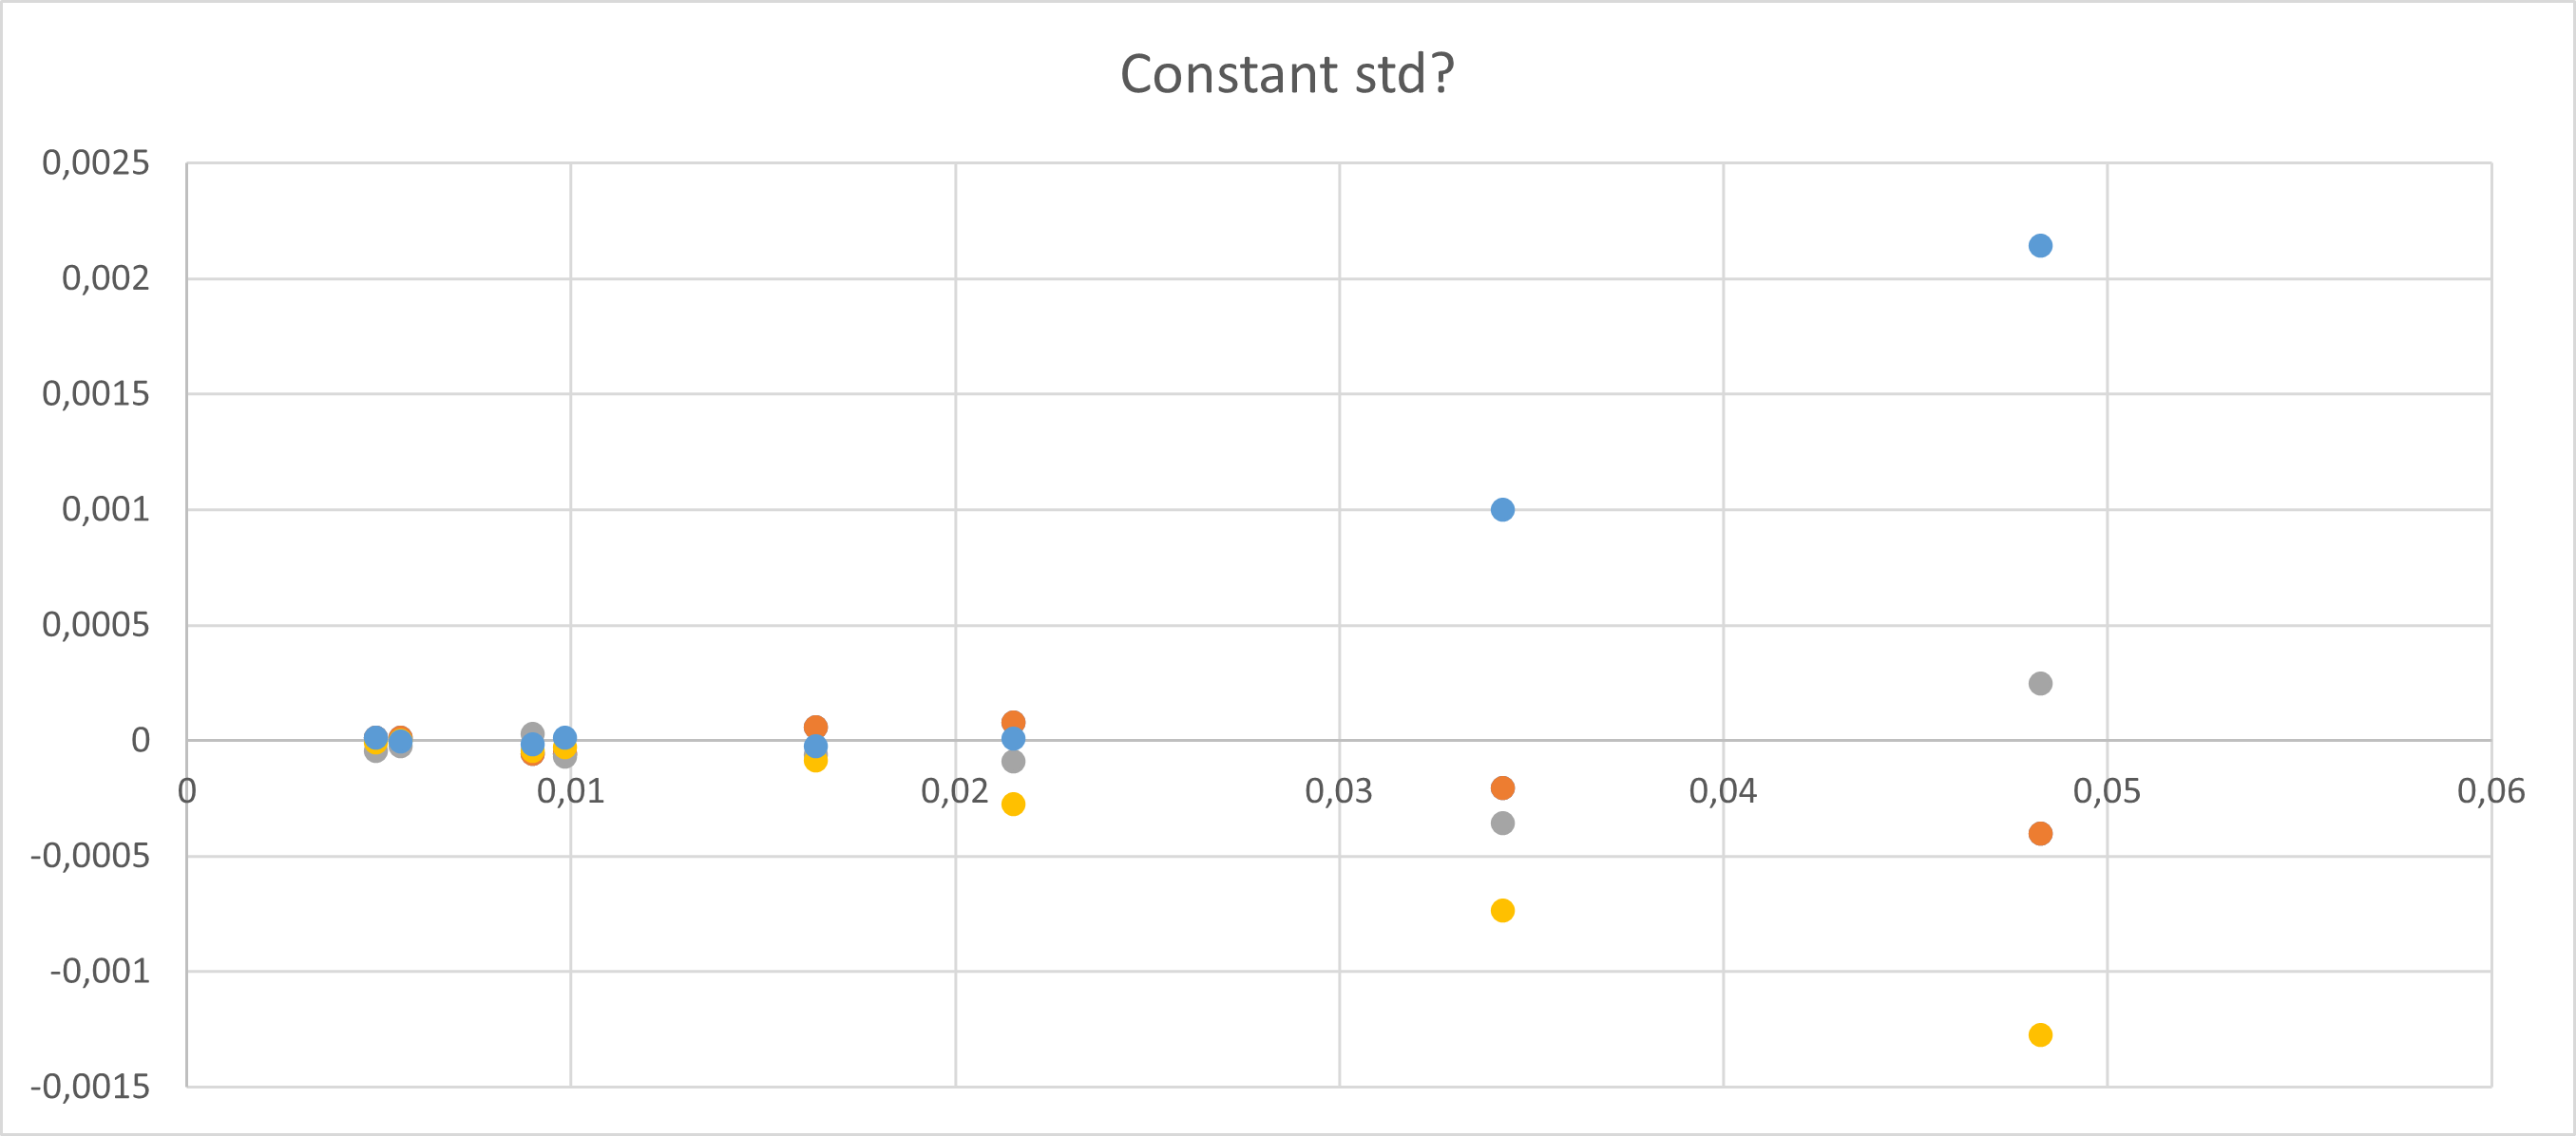
\includegraphics[scale=0.6]{images/standardDeviation_10.png}
                        \caption{Scatterplot for $Q = 10 S_t$}
                        \label{fig:standardDeviation_10}
                    \end{figure}
        
        \newpage
            \subsubsection{Case $Q = \frac{1}{10} S_t$}
            
                \paragraph{Results} \hfill \\
                \textit{Vacations} is the most affecting factor on the performance of the system, this is due to the fact that in this case the server needs more vacations to build up a turn big enough to serve an entire job, i.e. the bigger the vacation is, the higher will be the response time.
                It's also important to note that this system is very likely to be unstable since it's extremely sensible to small variations.

                    \begin{table}[htbp]
                        \centering 
                        \begin{tabular}{|c|c|c|c|c|c|c|c|}
                            \hline
                            \multicolumn{8}{|c|}{\bf Percentage of variation of the factors and the error} \\
                            \hline
                            \ $\lambda$ & $\mu$ & $\delta$ & $\lambda\mu$ & $\lambda\delta$ & $\mu\delta$ & $\lambda\mu\delta$ & $\epsilon$ \\
                            \hline
                            \ 0.38\% & 2.04\% & 95.29\% & 0.00\% & 0.36\% & 1.17\% & 0.00\% & 0.75\% \\ 
                            \hline
                        \end{tabular}
                        \label{table:variation_0,1}
                    \end{table}
                    
                    \begin{table}[htbp]
                        \begin{tabular}{|c|c|c|c|c|c|c|c|}
                        
                             \hline
                             \multicolumn{8}{|c|}{\bf Confidence interval with 98\% confidence level} \\
                                
                            \hline
                            \ & $\lambda$ & $\mu$ & $\delta$ & $\lambda\mu$ & $\lambda\delta$ & $\mu\delta$ & $\lambda\mu\delta$\\
                            \hline
                            \ CI- & -0.00847 & 0.00931 & 0.08180 & -0.00347 & -0.00835 & 0.00628 & -0.00343 \\ 
                            \hline
                            \ CI+ & -0.00226 & 0.01553 & 0.08801 & 0.00274 & -0.00213 & 0.01249 & 0.00277 \\ 
                            \hline
                        \end{tabular}
                        \label{table:CI_0,1}
                    \end{table}
                
                \paragraph{Testing hypothesis} \hfill \\
                The QQ plot can be assumed linear, meaning that the residuals are normal. About the standard deviation, even though it might show a trend, since residuals are one order of magnitude below the predicted response, we can consider it constant.
                
                    \begin{figure}[htbp]
                        \centering
                        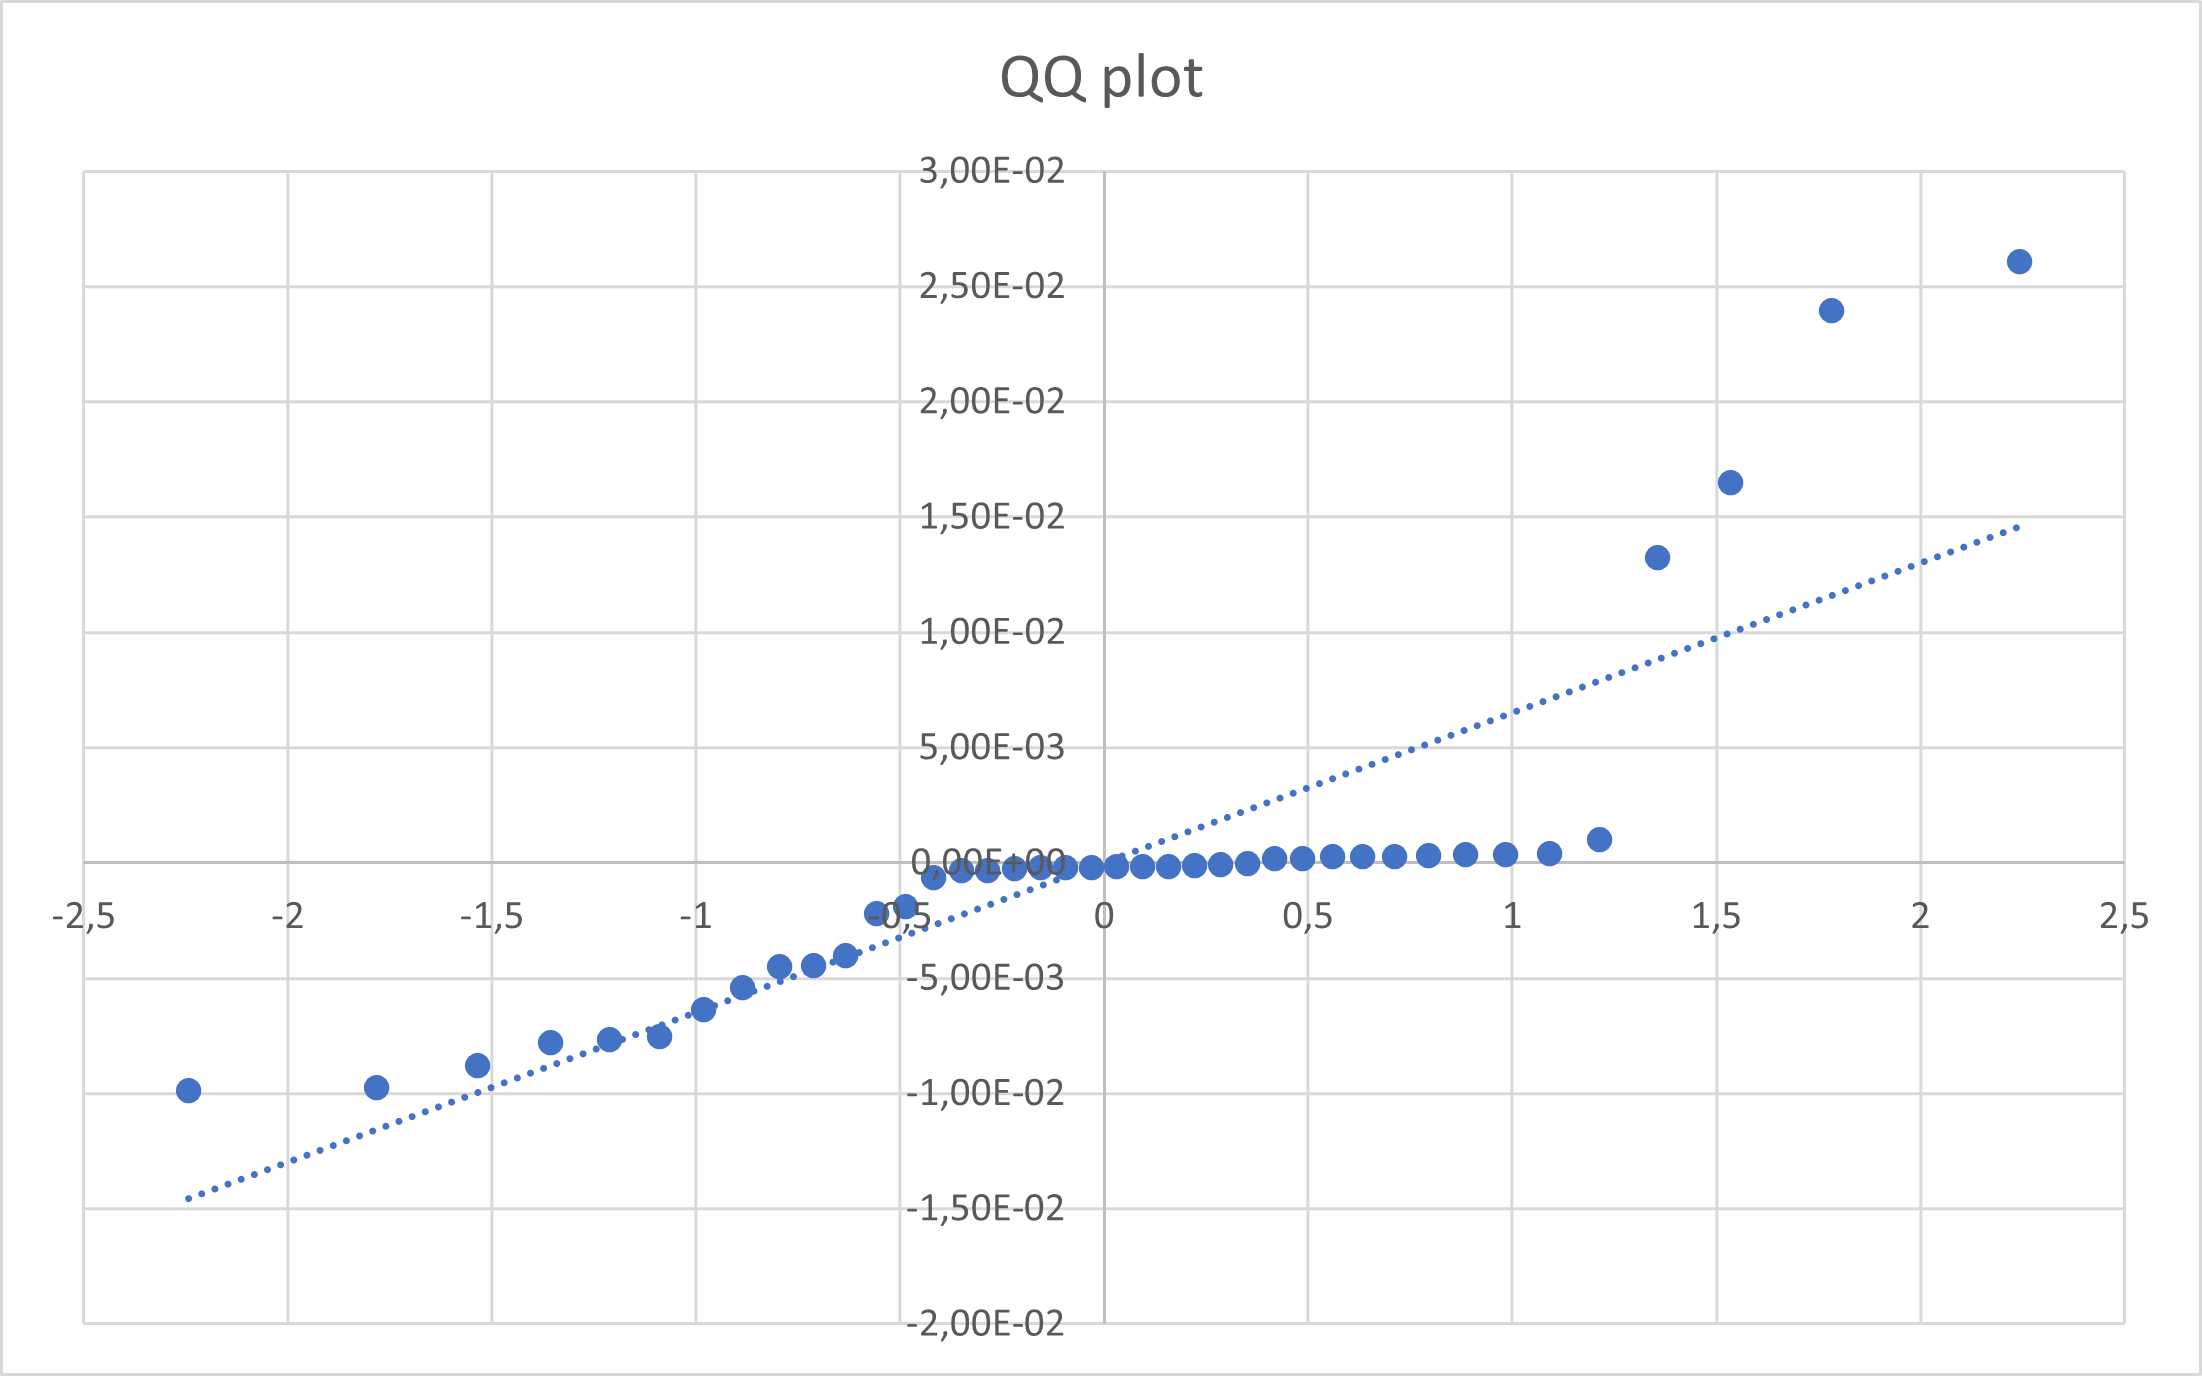
\includegraphics[scale=0.7]{images/QQplot_0,1.png}
                        \caption{QQ plot for $Q = \frac{S_t}{10}$}
                        \label{fig:QQplot_0,1}
                    \end{figure}
                    
                     \begin{figure}[htbp]
                        \centering
                        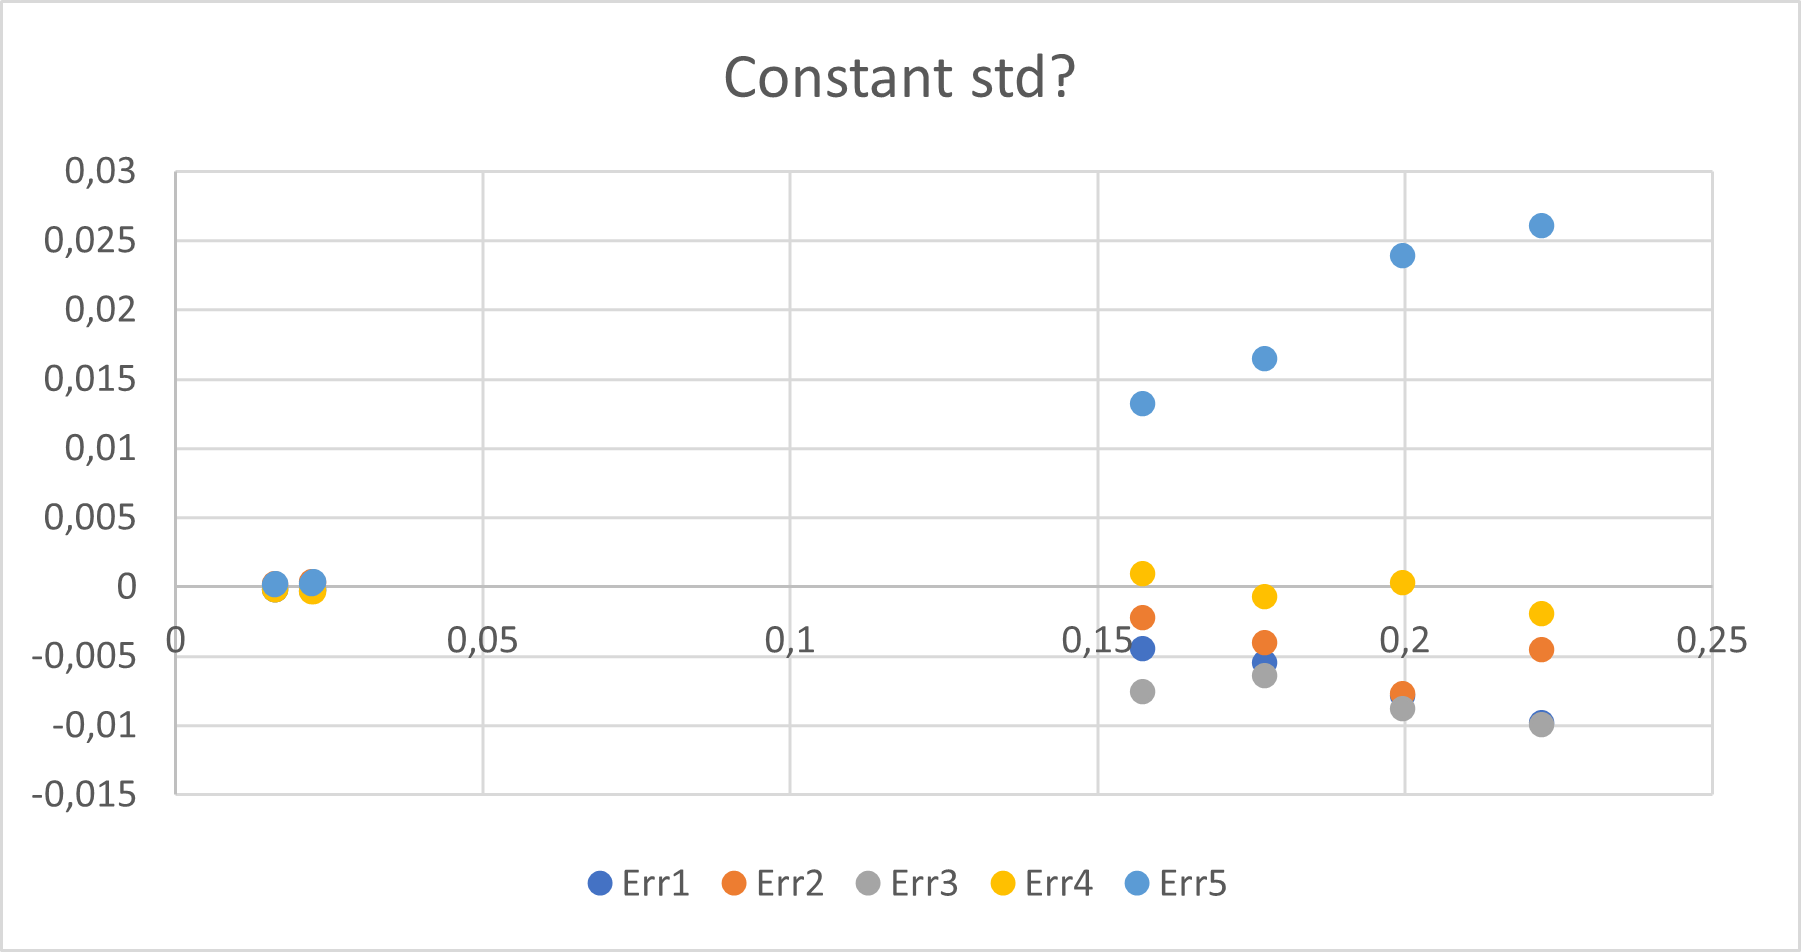
\includegraphics[scale=0.8]{images/standardDeviation_0,1.png}
                        \caption{Scatterplot for $Q = \frac{S_t}{10}$}
                        \label{fig:standardDeviation_0,1}
                    \end{figure}
                
        \newpage
        
        \subsubsection{Case $Q = \frac{1}{2} S_t$}
            
                \paragraph{Results} \hfill \\
                In this case we can easily see that \textit{Vacation} is the factor that most affects the system while the service time has got a lower impact. This leads to the conclusion that \textbf{the smaller the value of Q gets, the more the system is affected by the value of the vacation, while the service time becomes less relevant}.

                    \begin{table}[htbp]
                        \centering 
                        \begin{tabular}{|c|c|c|c|c|c|c|c|}
                            \hline
                            \multicolumn{8}{|c|}{\bf Percentage of variation of the factors and the error} \\
                            \hline
                            \ $\lambda$ & $\mu$ & $\delta$ & $\lambda\mu$ & $\lambda\delta$ & $\mu\delta$ & $\lambda\mu\delta$ & $\epsilon$ \\
                            \hline
                            \ 3.34\% & 18.65\% & 65.74\% & 1.28\% & 2.70\% & 7.12\% & 1.02\% & 0.14\% \\ 
                            \hline
                        \end{tabular}
                        \label{table:variation_0,5}
                    \end{table}
                    

                    \begin{table}[htbp]
                        \begin{tabular}{|c|c|c|c|c|c|c|c|}
                        
                            \hline
                            \multicolumn{8}{|c|}{\bf Confidence interval with 98\% confidence level} \\
                                
                            \hline
                            \ & $\lambda$ & $\mu$ & $\delta$ & $\lambda\mu$ & $\lambda\delta$ & $\mu\delta$ & $\lambda\mu\delta$\\
                            \hline
                            \ CI- & -0.00492 & 0.01033 & 0.01974 & -0.00319 & -0.00447 & 0.00623 & -0.00289 \\ 
                            \hline
                            \ CI+ & -0.00415 & 0.01111 & 0.02052 & -0.00242 & -0.00369 & 0.00701 & -0.00211 \\ 
                            \hline
                        \end{tabular}
                        \label{table:CI_0,5}
                    \end{table}
                    
                \paragraph{Testing hypothesis} \hfill \\
                Also in this case we can consider the assumptions as verified since the QQ plot in Figure \ref{fig:QQplot_0,5} can be assumed as linear.
                The same goes for the standard deviation that can be considered as constant since we can ignore the trend thanks to the fact that the errors are one order of magnitude below the predicted response.
                
                    \begin{figure}[htbp]
                        \centering
                        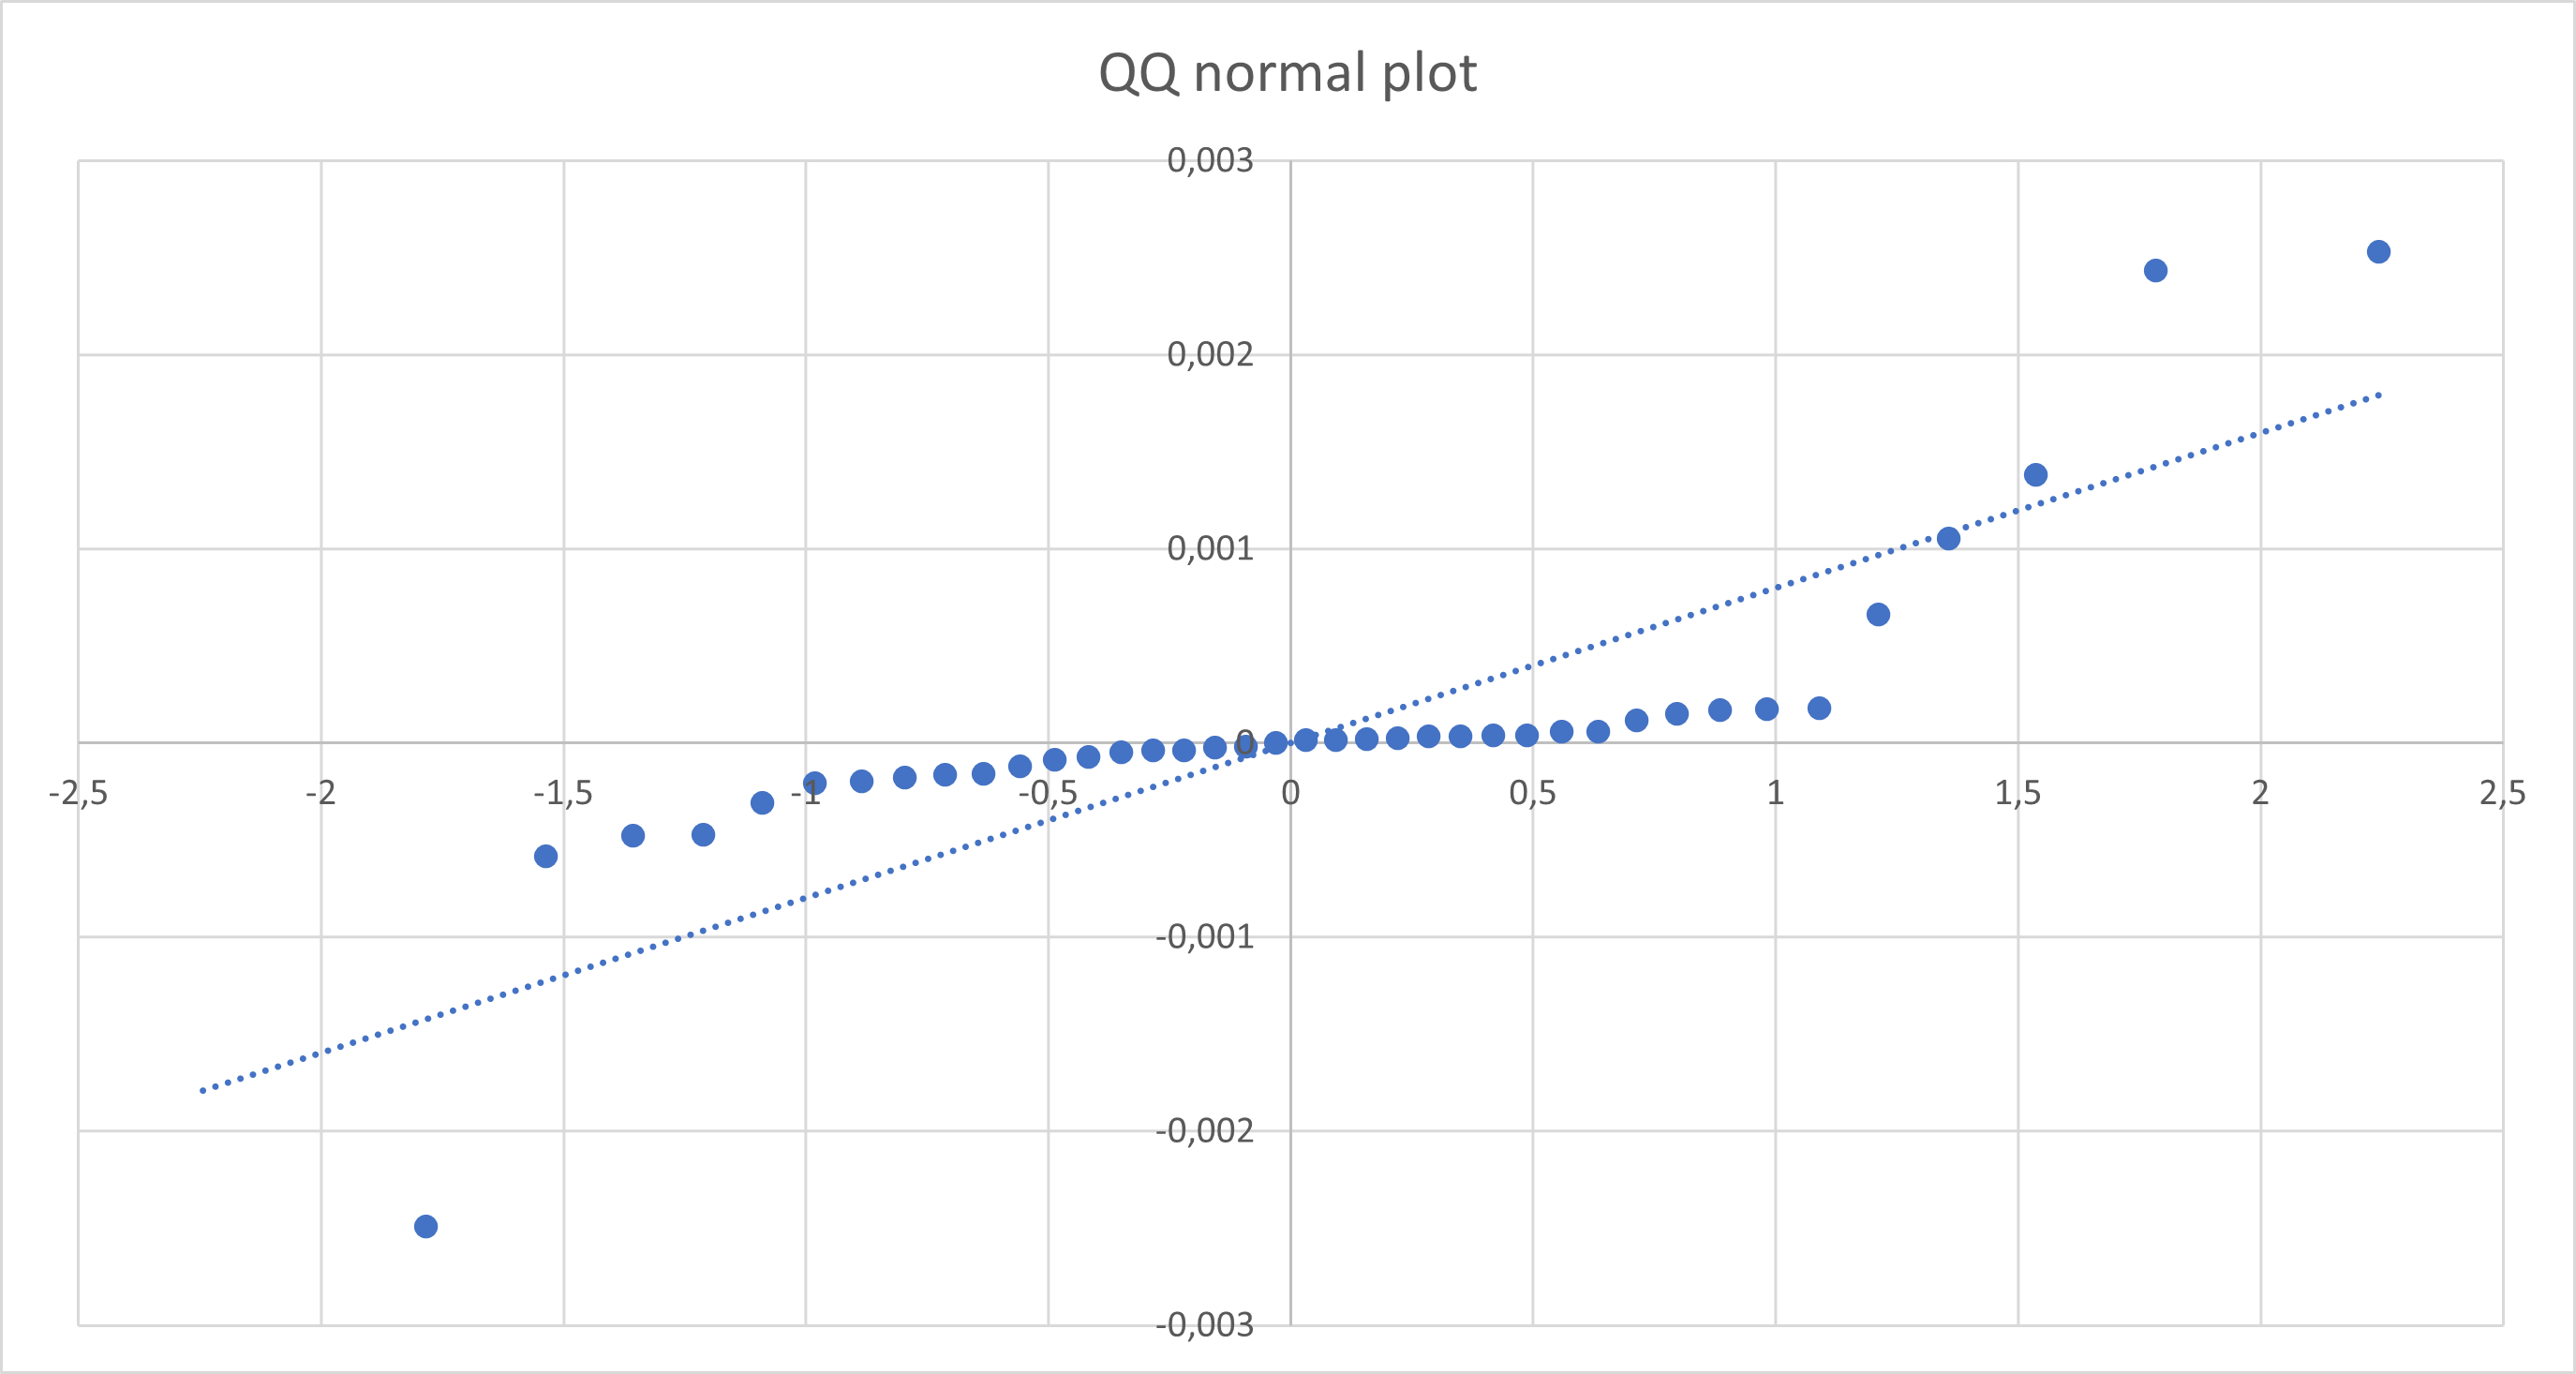
\includegraphics[scale=0.6]{images/QQplot_0,5.png}
                        \caption{QQ plot for $Q = \frac{S_t}{2}$}
                        \label{fig:QQplot_0,5}
                    \end{figure}
                    
                     \begin{figure}[htbp]
                        \centering
                        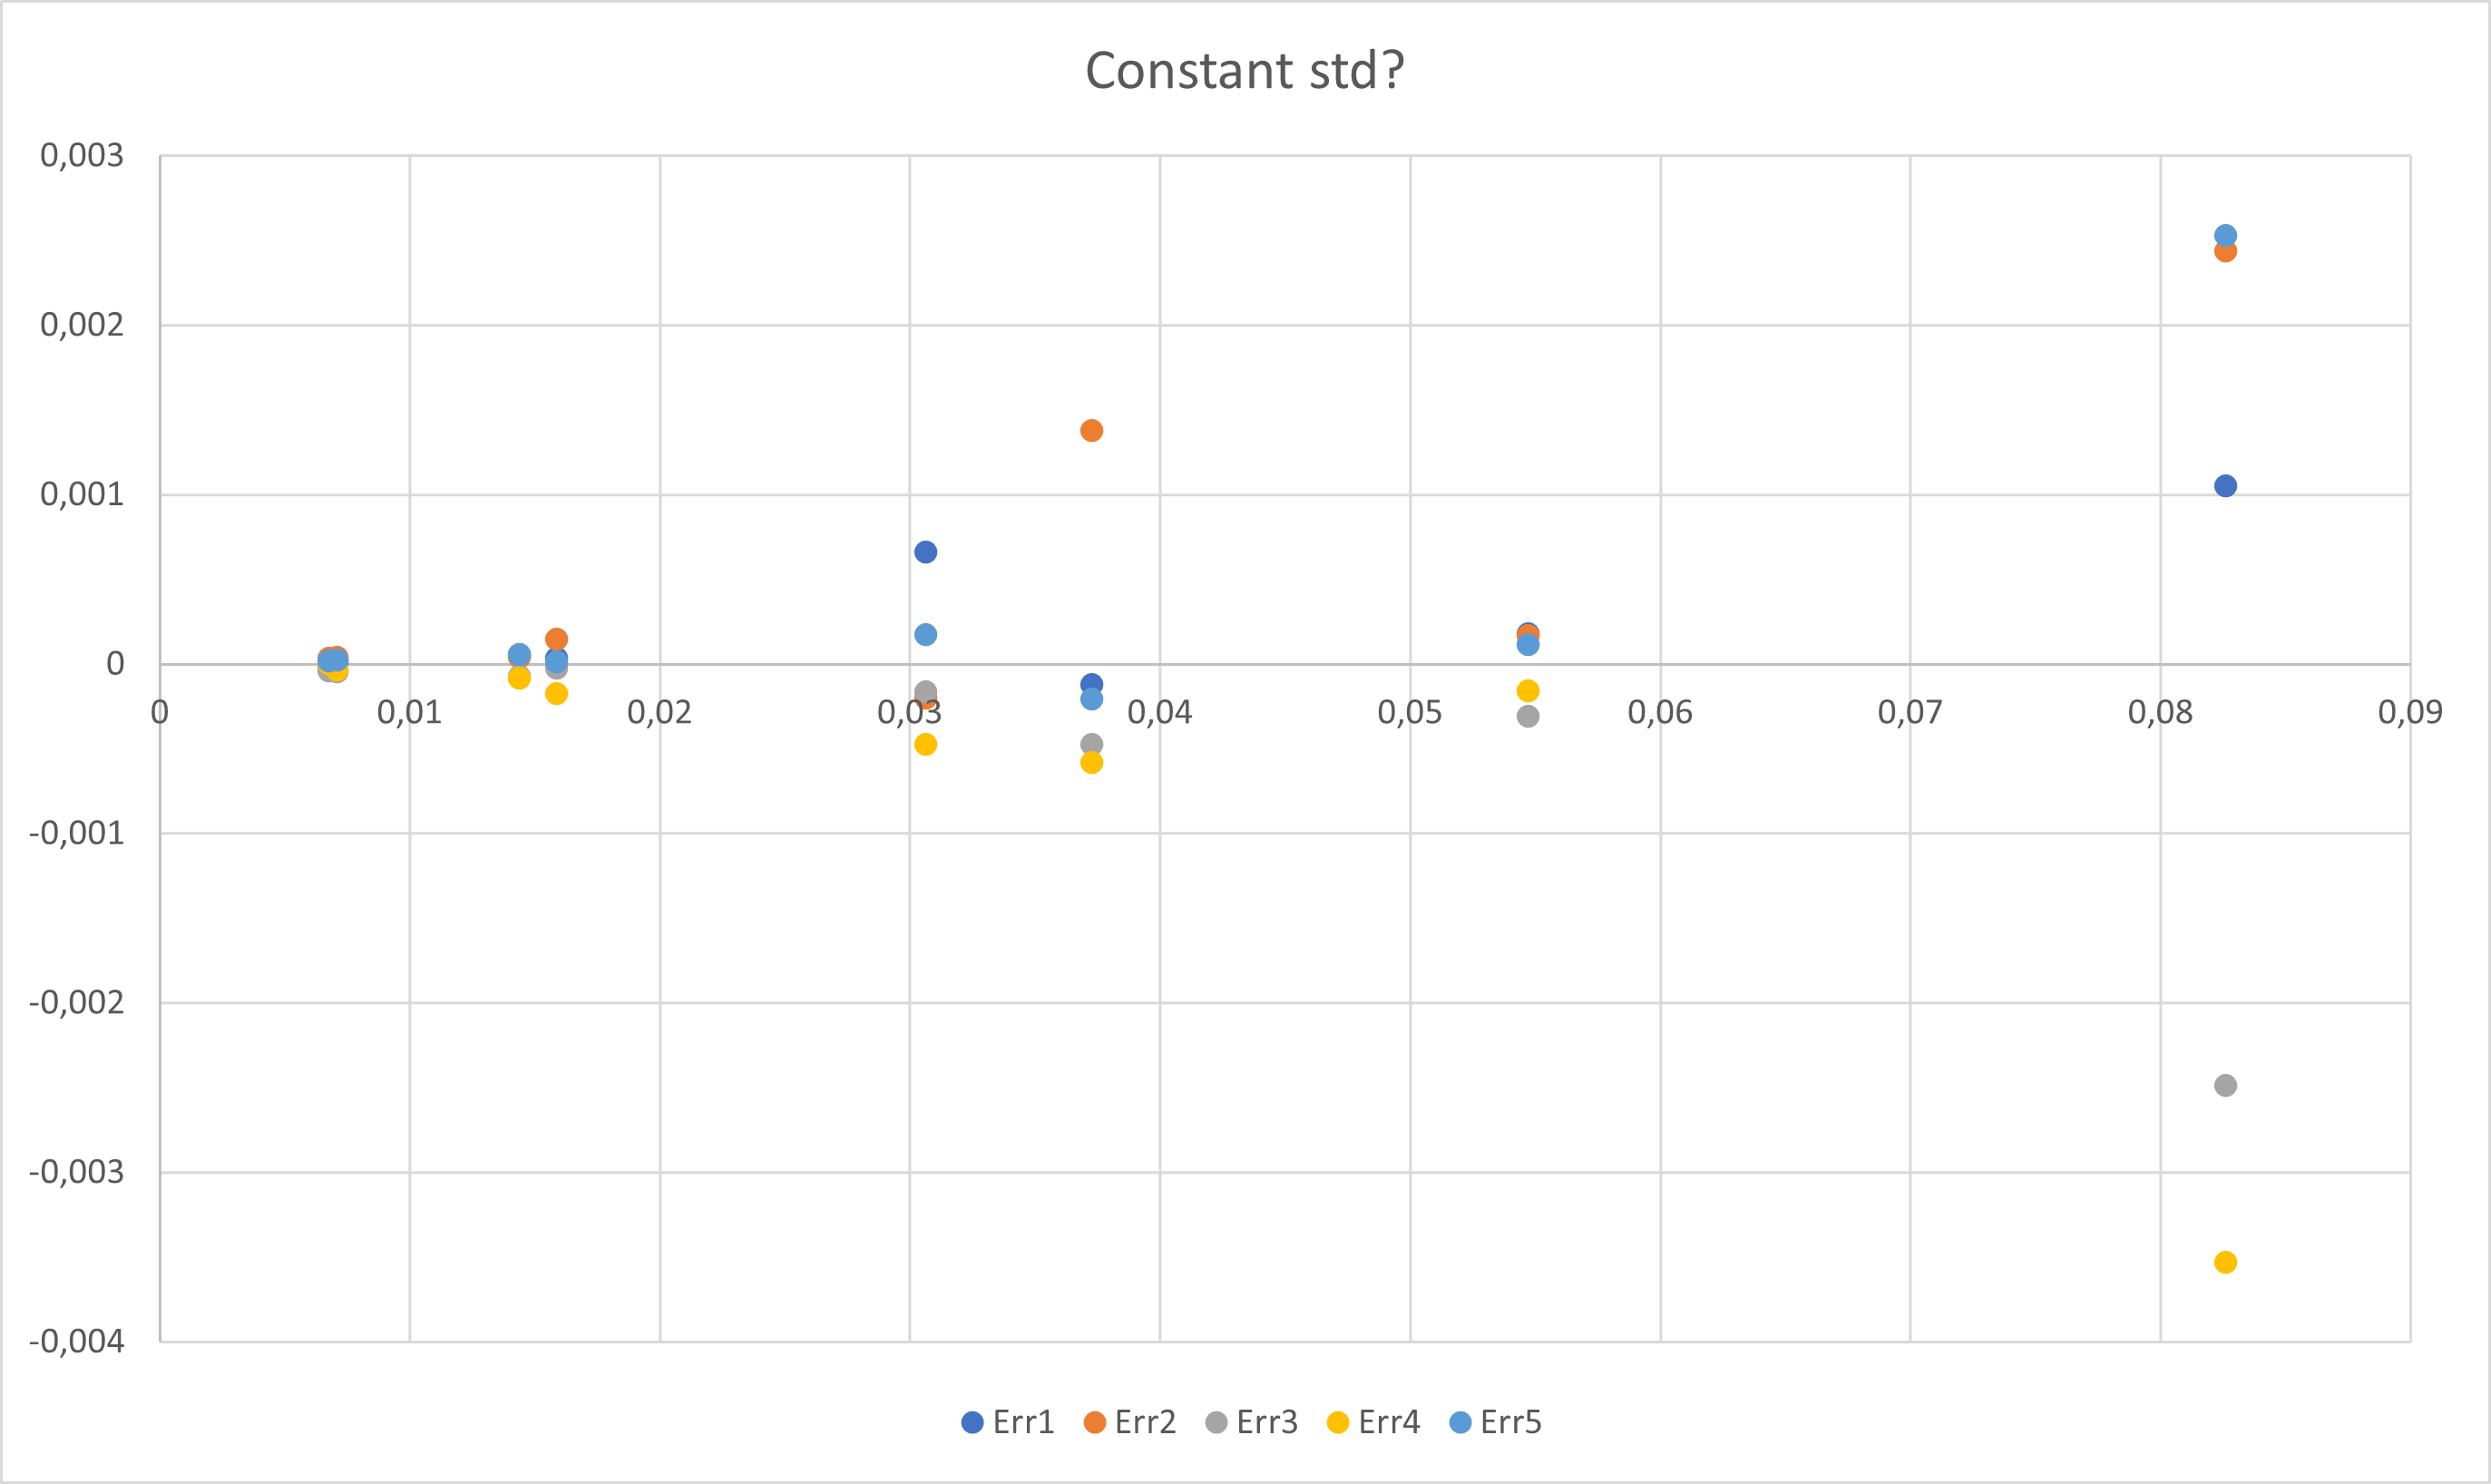
\includegraphics[scale=0.55]{images/standardDeviation_0,5.png}
                        \caption{Scatterplot for $Q = \frac{S_t}{2}$}
                        \label{fig:standardDeviation_0,5}
                    \end{figure}
                
        \newpage
        
        \subsubsection{Case $Q = 5S_t$}
            
                \paragraph{Results} \hfill \\
                
                In the case $Q = 5S_t$, the \textit{Service time} is the most affecting factor on the performance of the system. We can see that while Q grows, the impact of the service time becomes more important, and the vacation becomes less meaningful. This makes perfect sense, in fact for an increasing value of Q, the system becomes more and more close to an M/M/1, meaning that the vacation has a smaller impact on the response time.

                    \begin{table}[htbp]
                        \centering 
                        \begin{tabular}{|c|c|c|c|c|c|c|c|}
                            \hline
                            \multicolumn{8}{|c|}{\bf Percentage of variation of the factors and the error} \\
                            \hline
                            \ $\lambda$ & $\mu$ & $\delta$ & $\lambda\mu$ & $\lambda\delta$ & $\mu\delta$ & $\lambda\mu\delta$ & $\epsilon$ \\
                            \hline
                            \ 12.11\% & 61.26\% & 11.72\% & 10.00\% & 1.38\% & 2.30\% & 1.15\% & 0.07\% \\ 
                            \hline
                        \end{tabular}
                        \label{table:variation_5}
                    \end{table}
                    
                    \begin{table}[htbp]
                        \begin{tabular}{|c|c|c|c|c|c|c|c|}
                        
                            \hline
                            \multicolumn{8}{|c|}{\bf Confidence interval with 98\% confidence level} \\
                                
                            \hline
                            \ & $\lambda$ & $\mu$ & $\delta$ & $\lambda\mu$ & $\lambda\delta$ & $\mu\delta$ & $\lambda\mu\delta$\\
                            \hline
                            \ CI- & -0.00450 & 0.00969 & 0.00416 & -0.00410 & -0.00160 & 0.00177 & -0,00147 \\ 
                            \hline
                            \ CI+ & -0.00423 & 0.00995 & 0.00443 & -0.00383 & -0.00134 & 0.00203 & -0.00121 \\ 
                            \hline
                        \end{tabular}
                        \label{table:CI_5}
                    \end{table}
                
                \paragraph{Testing hypothesis} \hfill \\
                Once again the QQ plot looks approximately linear and the constant standard deviation assumption can be held by the fact that residuals are orders of magnitude smaller that the predicted response.
                
                    \begin{figure}[htbp!]
                        \centering
                        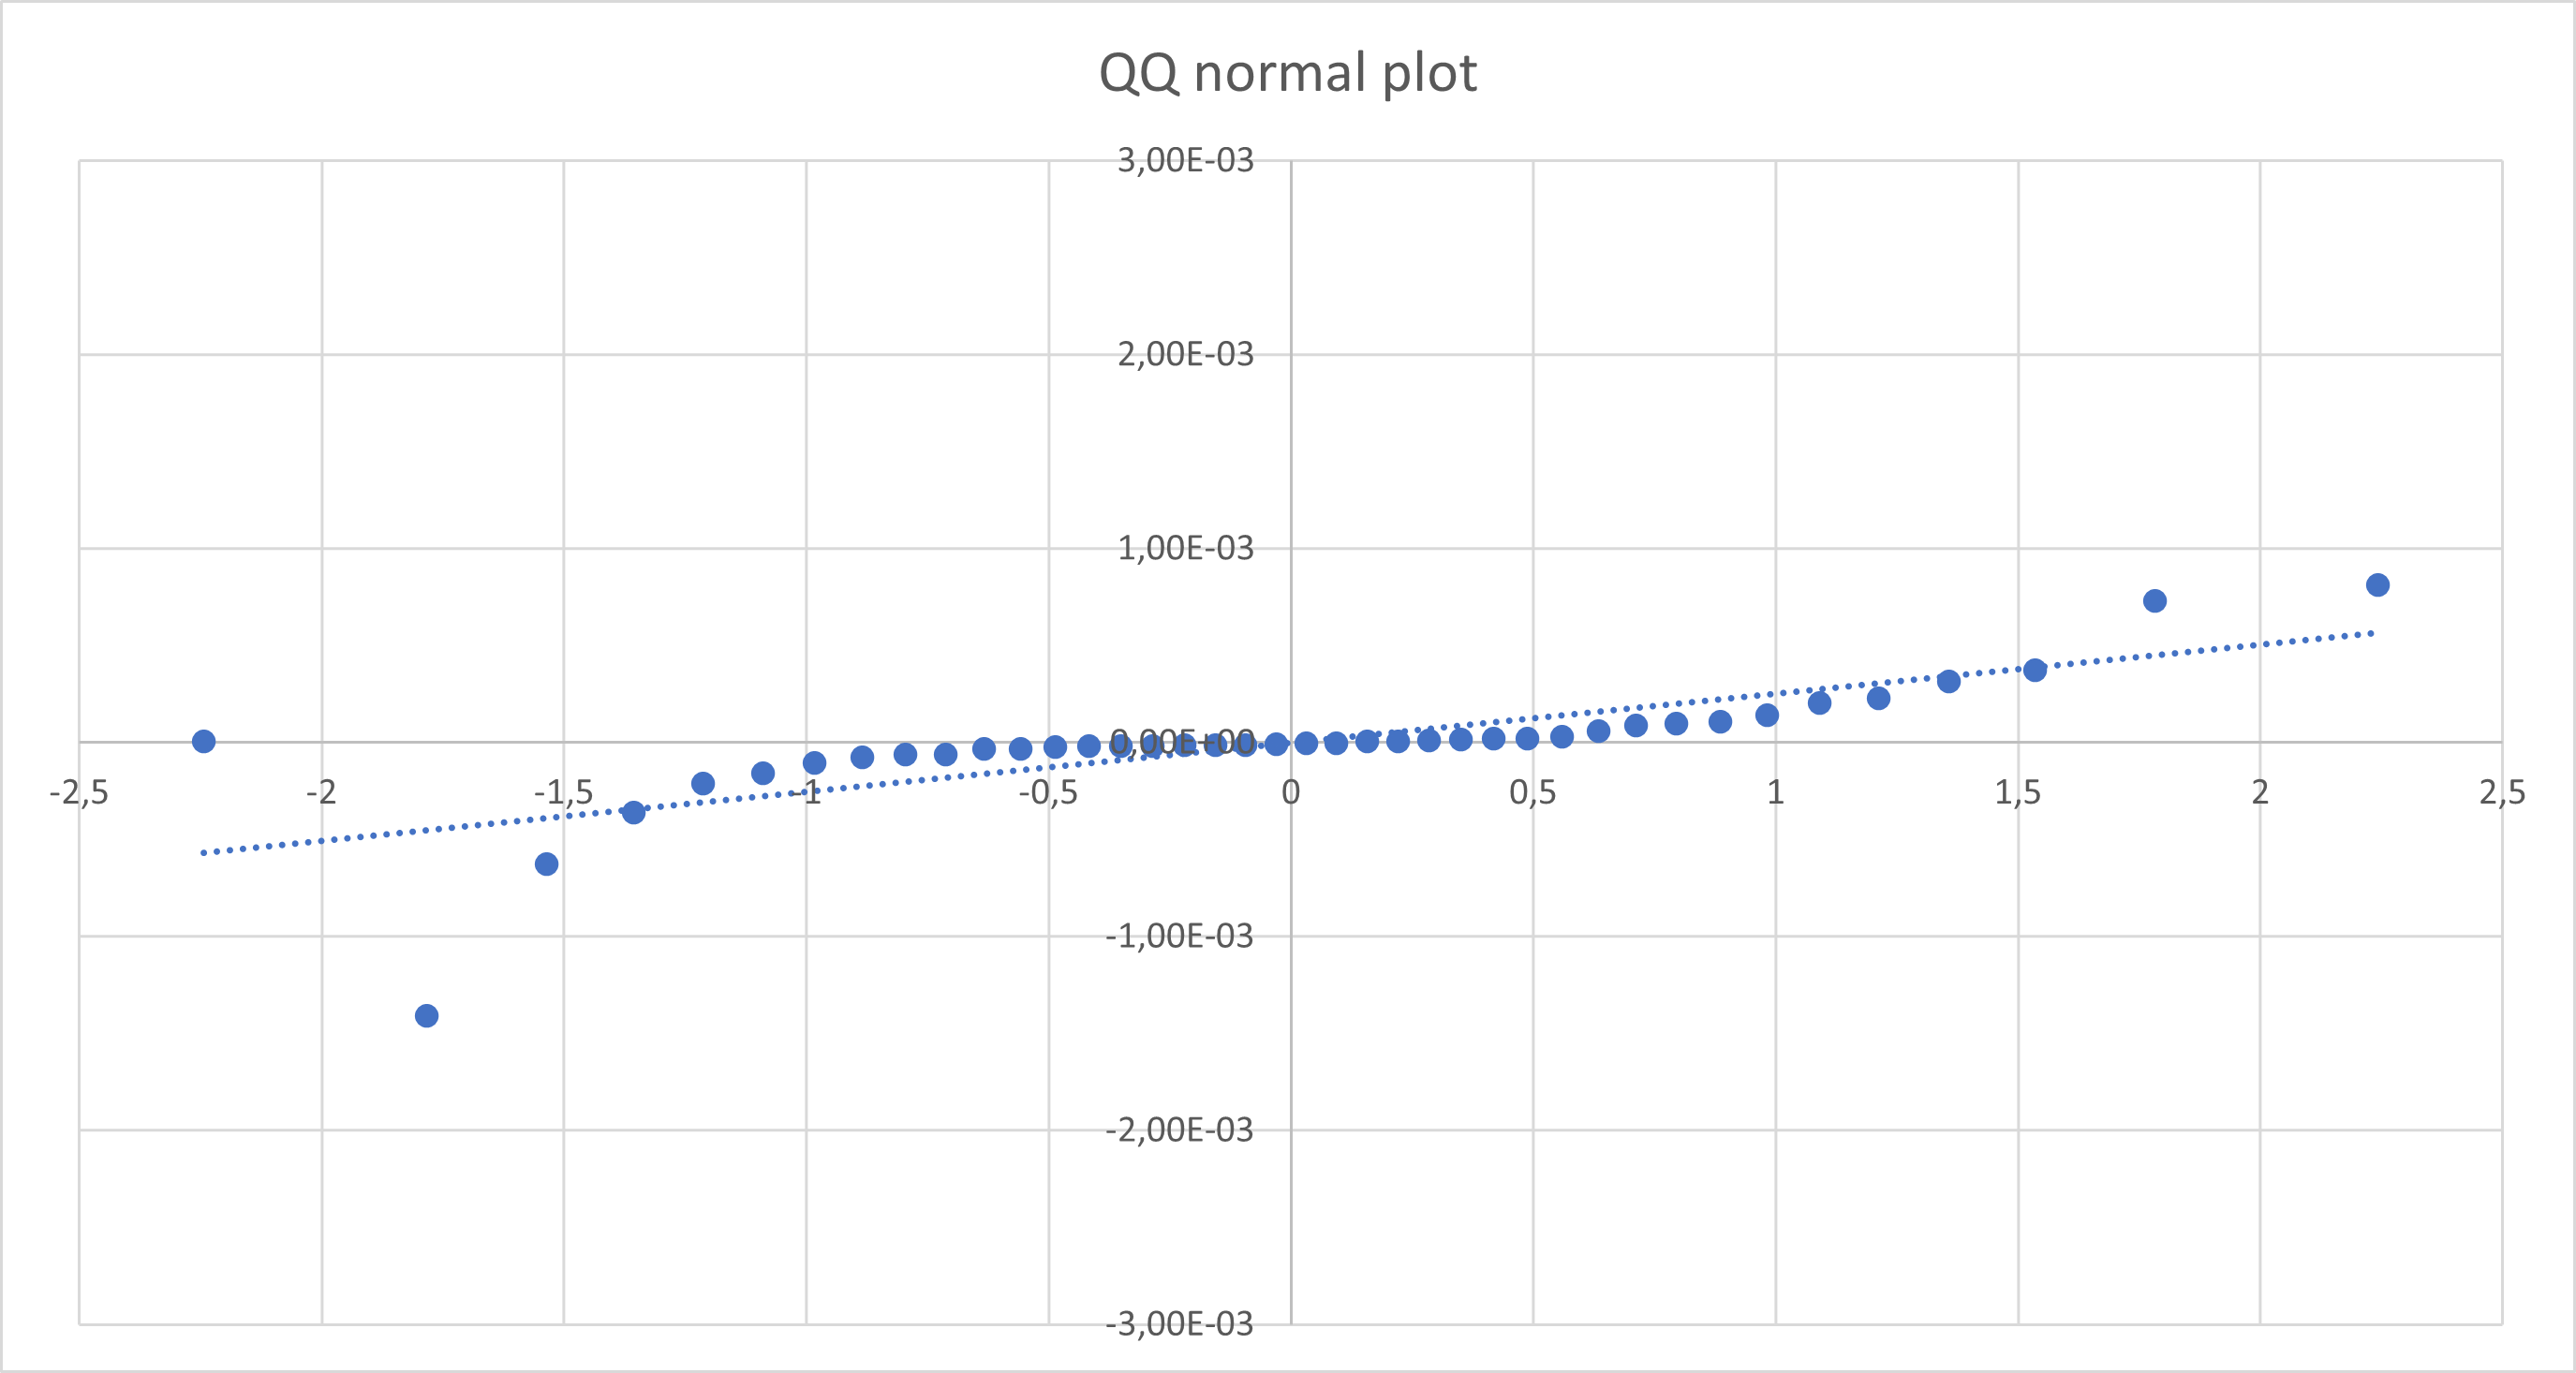
\includegraphics[scale=0.6]{images/QQplot_5.png}
                        \caption{QQ plot for $Q = 5{S_t}$}
                        \label{fig:QQplot_5}
                    \end{figure}
                    
                     \begin{figure}[htbp!]
                        \centering
                        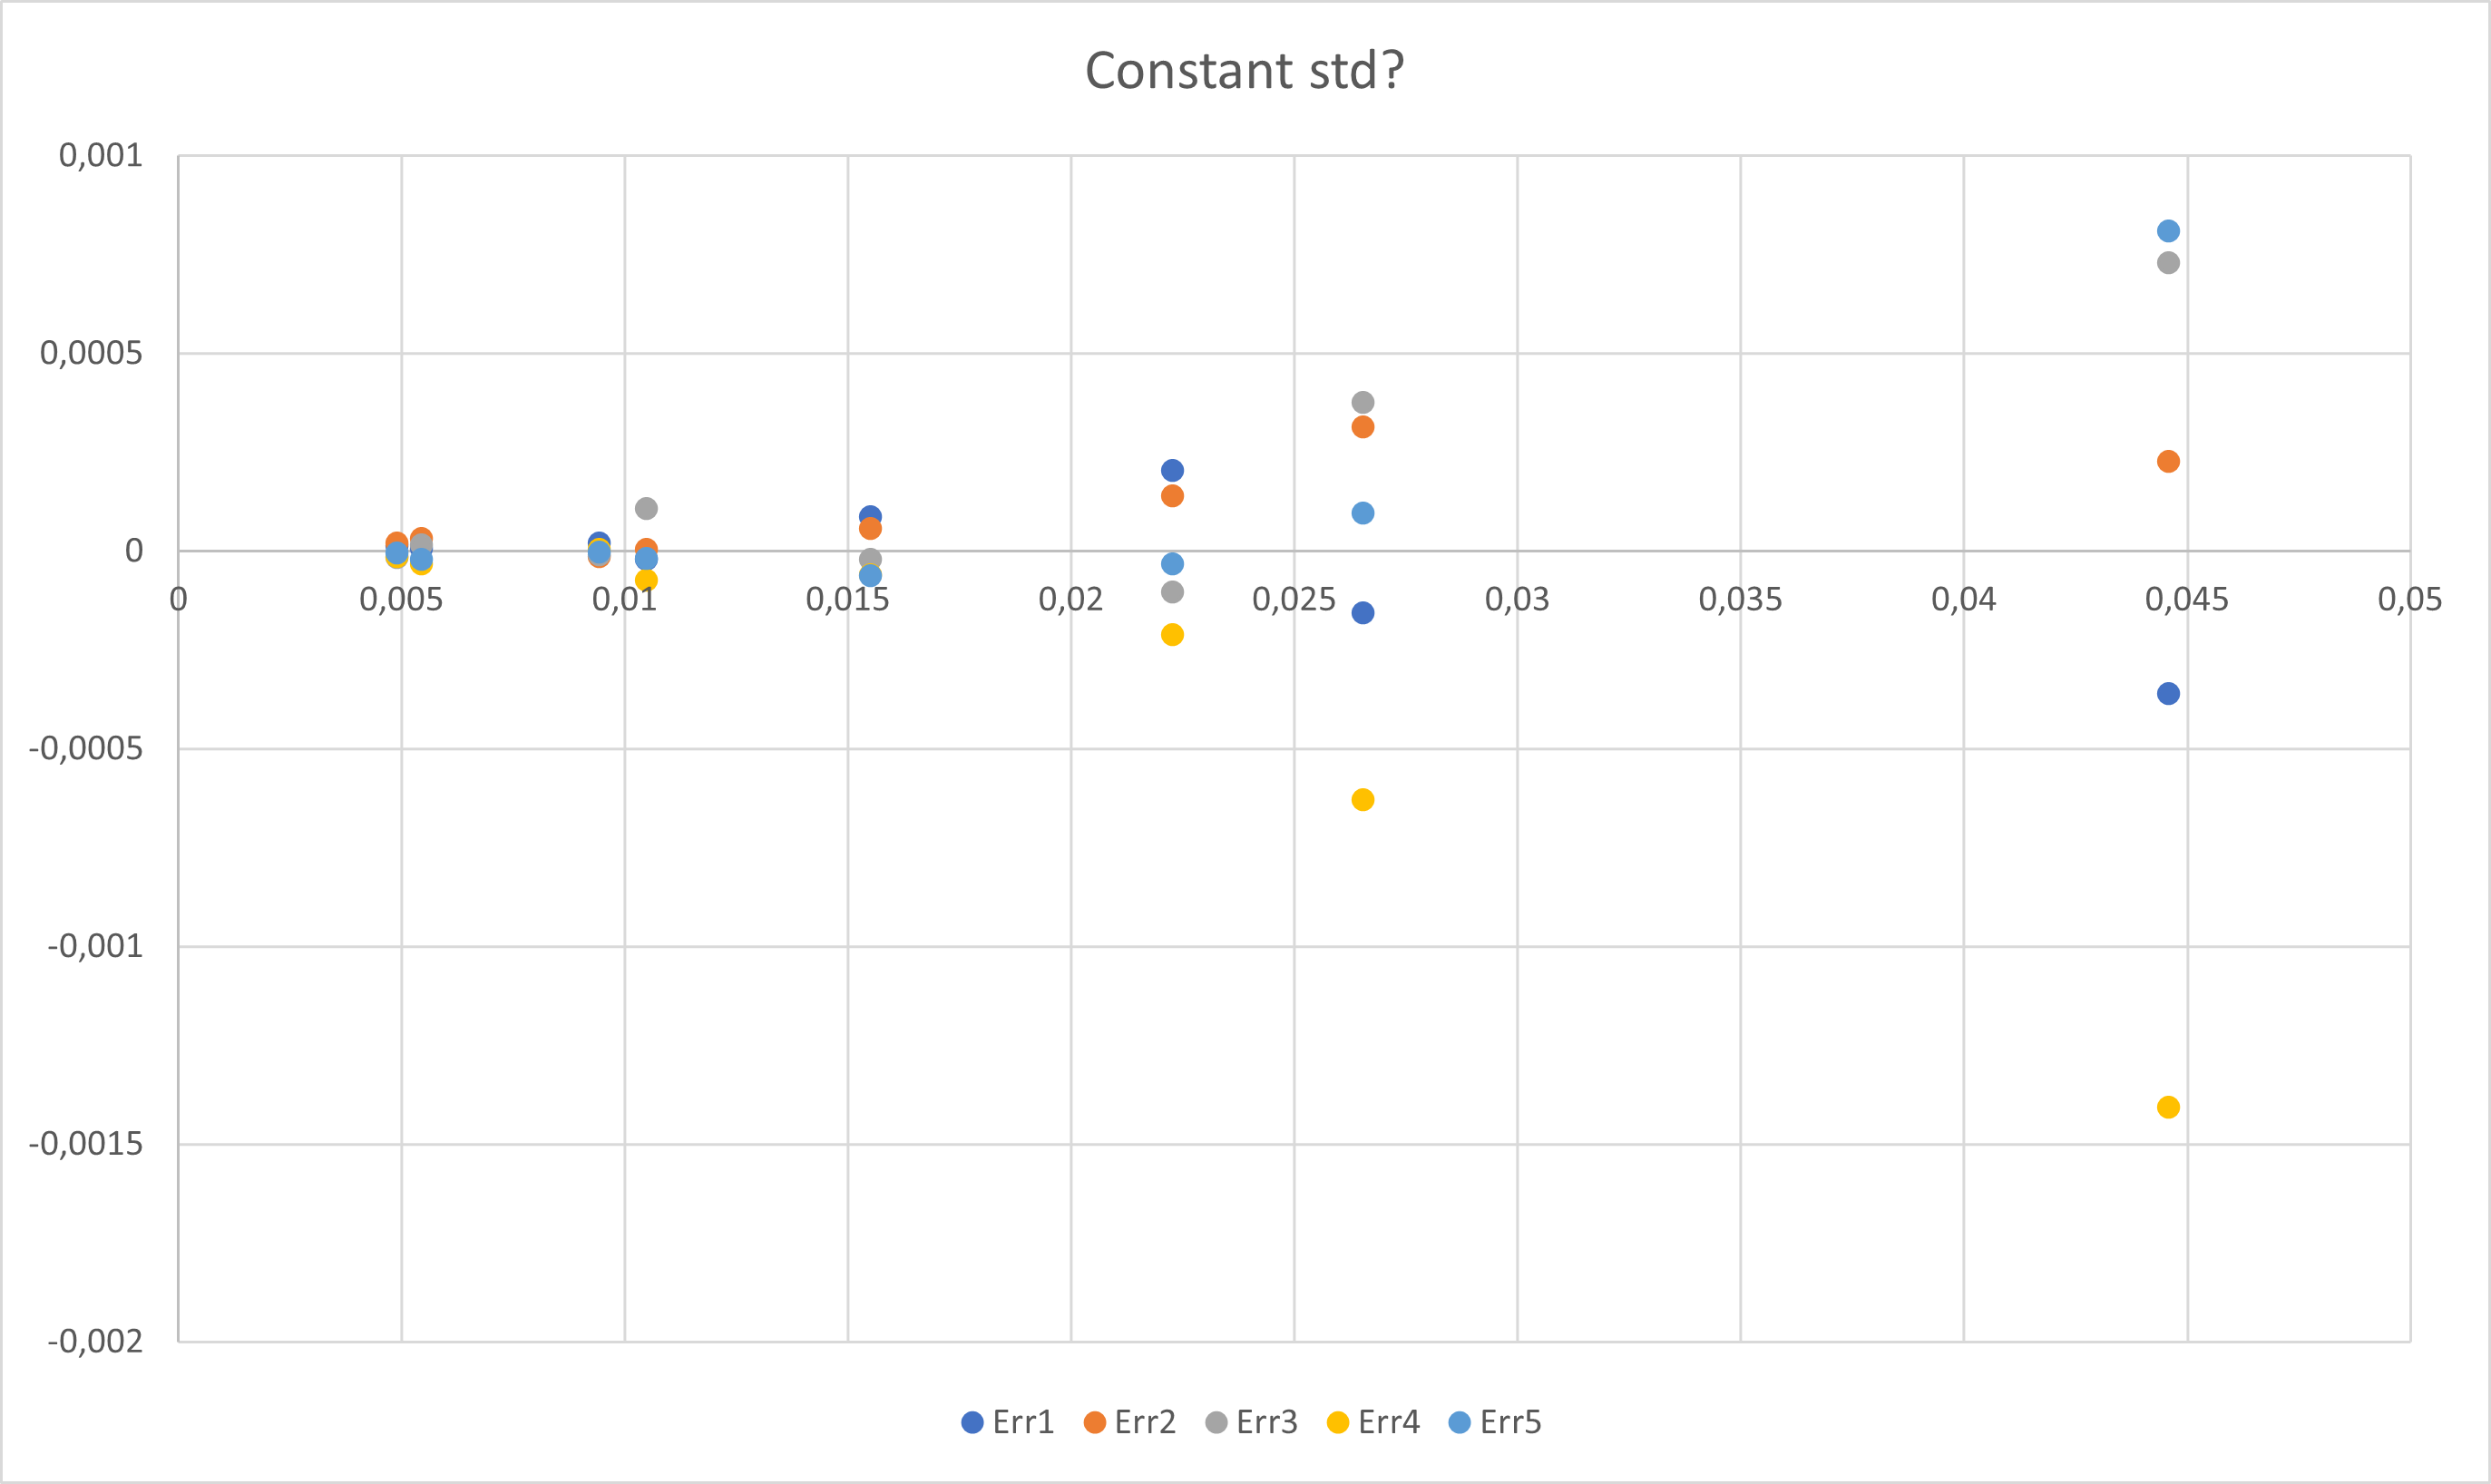
\includegraphics[scale=0.55]{images/standardDeviation_5.png}
                        \caption{Scatterplot for $Q = 5{S_t}$}
                        \label{fig:standardDeviation_5}
                    \end{figure}
                    
    \newpage
    
    \section{Data Analysis for the Exponential case}
        Once we obtained the results from the $2^k r$ analysis, we exploited them in the data analysis, with the aim of getting some insights on the system and doing different model fittings.\\

        In order to perform the fitting we ran $15$ replicas for each scenario of interest, meaning that we only changed the values of the factors that had most impact on the system. Out of the 15 replicas we took the average response time, and then from those we computed the sample mean, variance and CoV. We used QQ plots in order to test the assumption of normality and computed the confidence intervals for every sample mean. Then we took the sample mean for each scenario and tried to find a model that fitted our results. None of them looked linear at all, but after a simple transformation we managed to fit them into a linear model that allowed us to predict, with a specific confidence range, the average behavior of our system when varying one or two factors inside the range of interest.
        For each regression we computed the confidence interval for the slope, the offset and for the predicted response, with a confidence level of 95\%.

\newpage
        \subsection{Case $Q = \frac{1}{10}S_t$}
            As a result of the $2^k r$ analysis we obtained that the factor with the higher variation was $\delta$ ($95,29\%$ of variation) so we used fixed values for inter-arrival time and service time while we made the vacation varying between $1ms$ and $5ms$ with steps of $0.25ms$. 
            
            \subsubsection{Linear regression for $\delta$}
                \paragraph{Settings for the simulations} \hfill \\
                    \lstinputlisting[language=Octave]{txt_ini/Q01_delta.txt}
                    
                \paragraph{Fitting} \hfill \\
                    Plotting the mean of the response time of each scenario against the values of $\delta$, we noticed that the distribution was perfectly fitting an exponential (Figure \ref{fig:Q01_exp_delta}), then we applied a transformation in order to fit the distribution with a linear model (Figure \ref{fig:Q01_lin_delta}) and in the end we tested the assumptions and we verified that the assumptions were met. \\
                    
                    The result obtained can be explained by the fact that when you increase the value of the vacation the mean response time will suffer a huge increase, since for smaller values of Q the system will need a larger number of vacations in order to build a turn big enough to serve one job.\\
                    
                    Moreover, the model is also valid for values outside our case study range, for big $\delta$s the system is unstable and the model approaches $\infty$, while \textbf{for small values of $\delta$, the system behaves like an M/M/1}, and exactly like one in which the vacation is null, meaning that the mean response time will be like the theoretical one. Our regression model tends to that value for $\delta \rightarrow 0$.
                    
                    \begin{figure}[htbp!]
                        \centering
                        \begin{minipage}[c]{.40\textwidth}
                            \centering
                            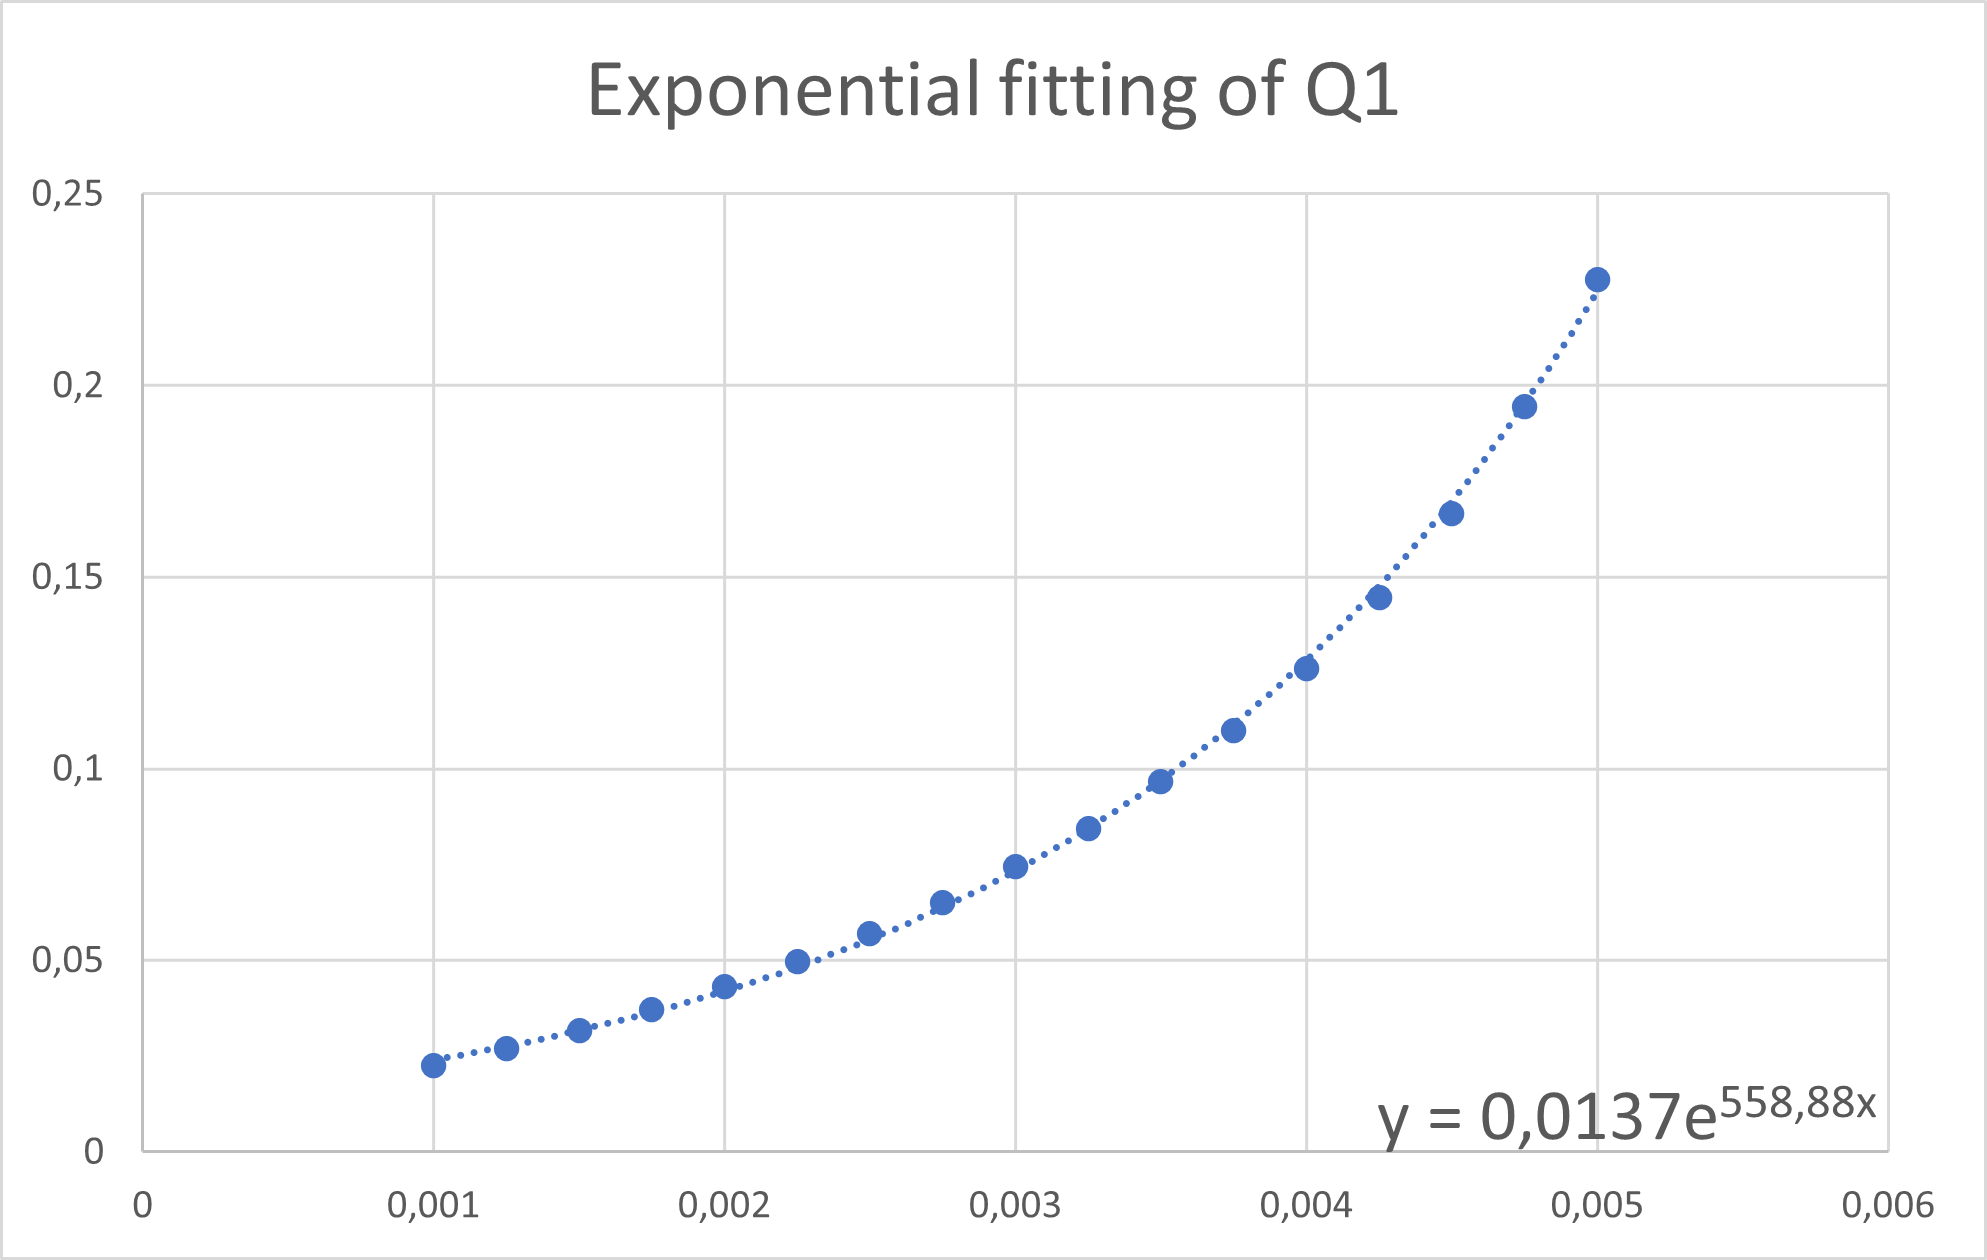
\includegraphics[width=\textwidth]{./data_analysis/Q01_exp_delta.png}
                            \caption{Fitting with the exponential}
                            \label{fig:Q01_exp_delta}
                        \end{minipage}
                        \hspace{10mm}
                        \begin{minipage}[c]{.40\textwidth}
                            \centering
                            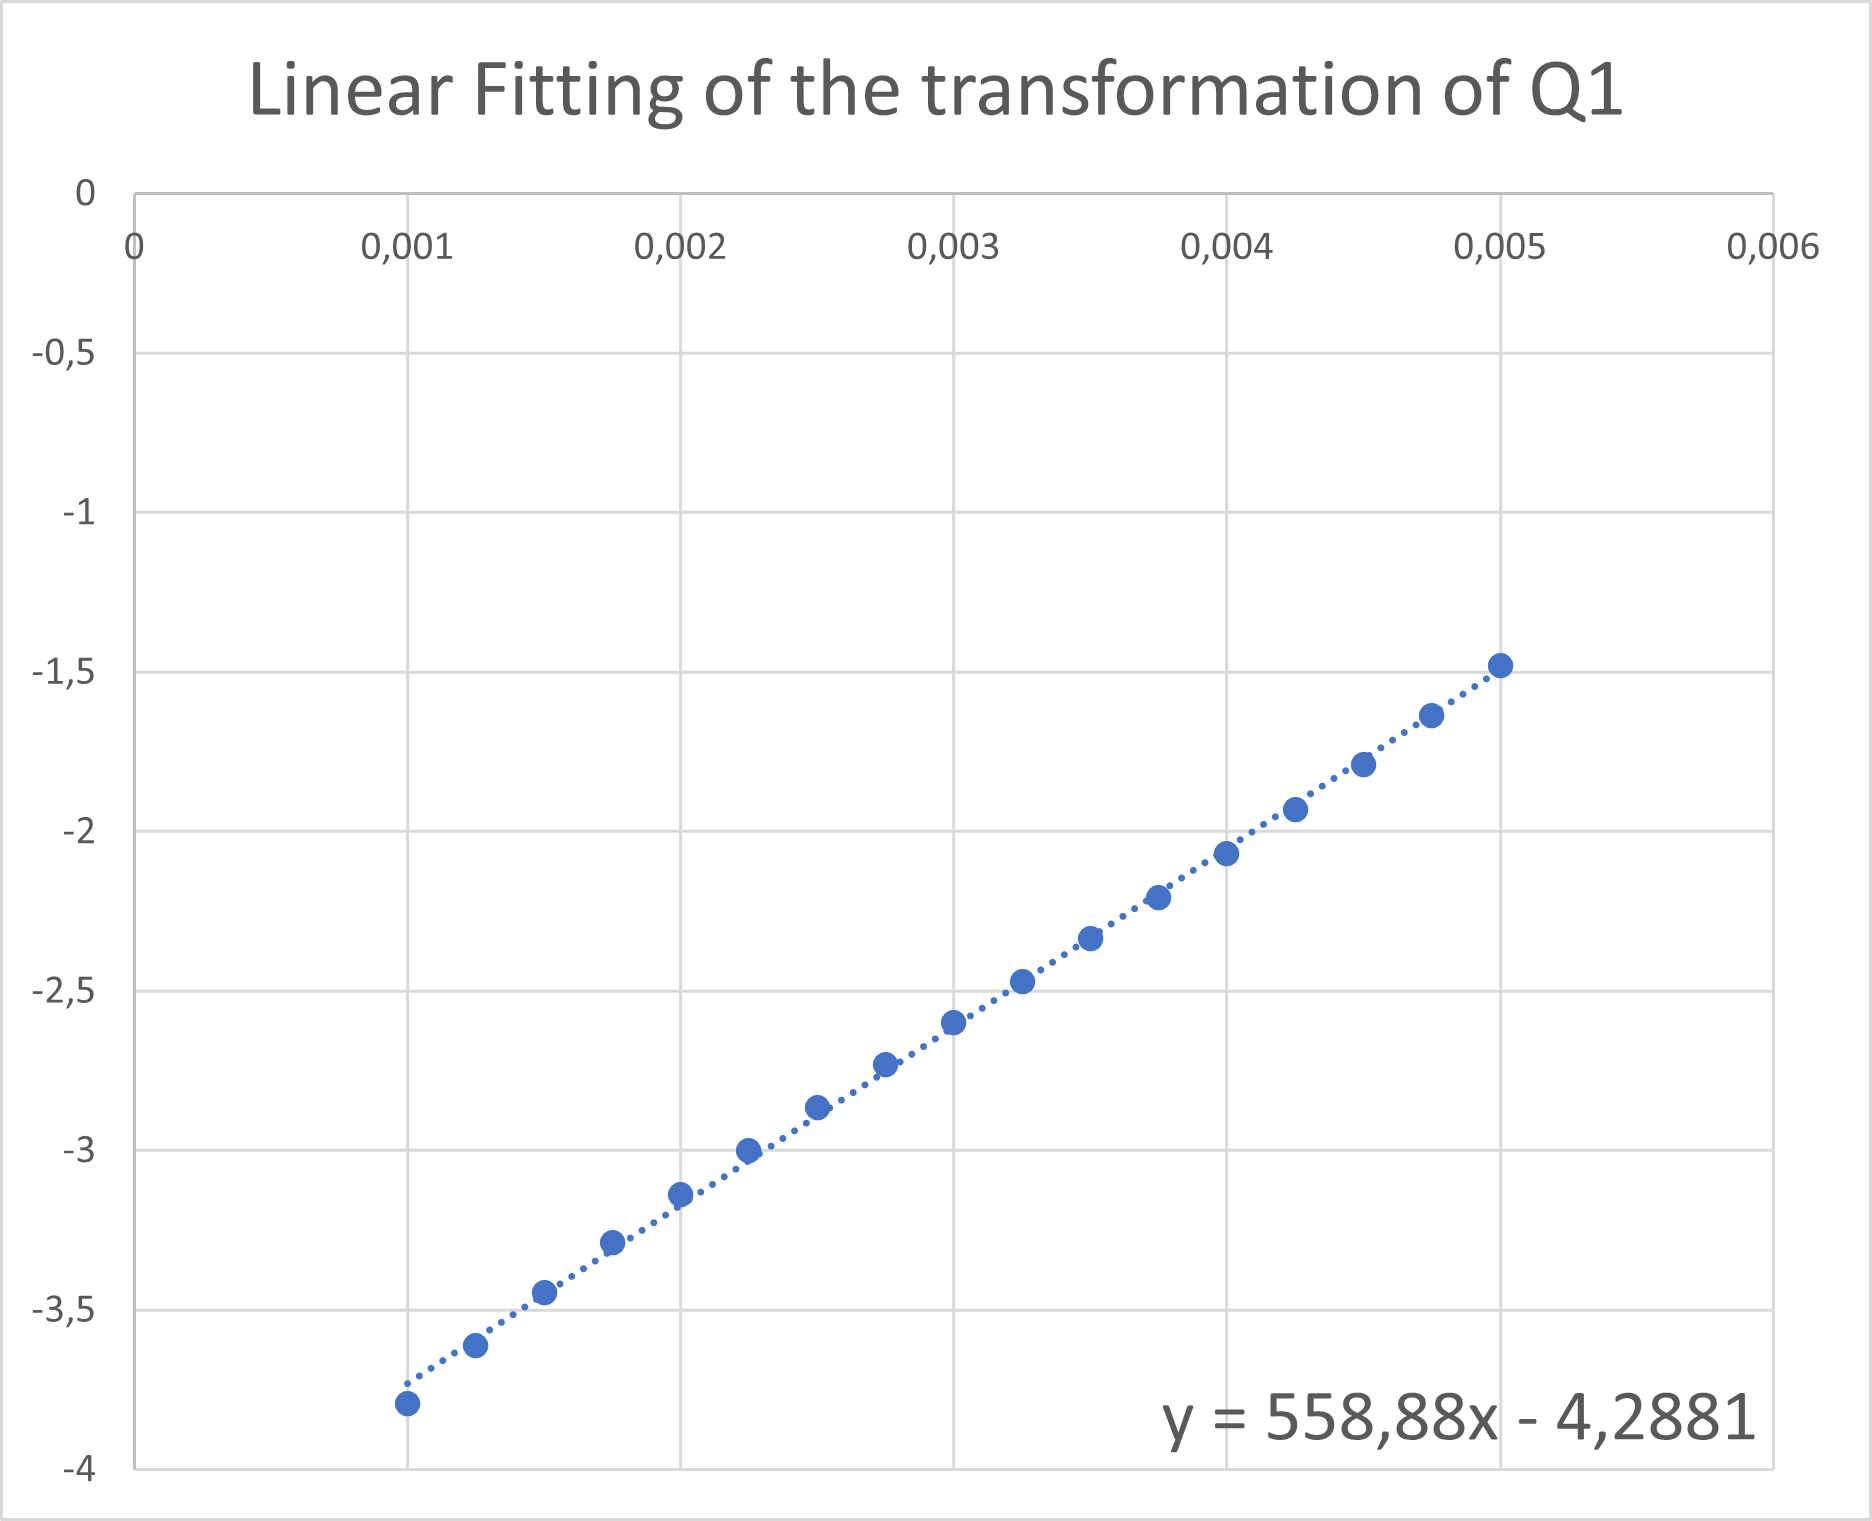
\includegraphics[width=\textwidth]{./data_analysis/Q01_lin_delta.png}
                            \caption{Transformation of the exponential for linear regression}
                            \label{fig:Q01_lin_delta}
                        \end{minipage}
                    \end{figure}
                    
                    \begin{table}[htbp]
                        \centering 
                        \begin{tabular}{|c|c|c|}
                            
                            \hline
                            \multicolumn{3}{|c|}{\bf Confidence interval with 95\% confidence level} \\
                            
                            \hline
                            \ & Slope & Offset\\
                            \hline
                            \ Upper Limit & 558.8994146 & -4.275803281 \\ 
                            \hline
                            \ Lower Limit & 558.8605854 & -4.300396719 \\ 
                            \hline
                        \end{tabular}
                        \label{table:CI_01_fitting}
                    \end{table}
    \newpage               
        \subsection{Case $Q = \frac{1}{2}S_t$}
            In this case what we got was that $\delta$ accounted for the $65,74\%$ of the variation, so we fixed the inter-arrival time and service time and changed the vacation between $1ms$ and $5ms$ with steps of $0.5ms$. 
            \subsubsection{Linear regression for $\delta$}
                \paragraph{Settings for the simulation} \hfill \\
                    \lstinputlisting[language=Octave]{txt_ini/Q05_delta.txt}
                \paragraph{Fitting} \hfill \\

                    From Figure \ref{fig:Q05_exp_delta} we can see that the distribution of the mean of the means of the response time obtained by varying $\delta$, is fitting well the exponential, for the same reasons of the previous case.\\
                    
                    In Figure \ref{fig:Q05_lin_delta} it is shown the transformation of the exponential applied in order to perform the linear fitting.             
                    \begin{figure}[htbp!]
                        \centering
                        \begin{minipage}[c]{.40\textwidth}
                            \centering
                            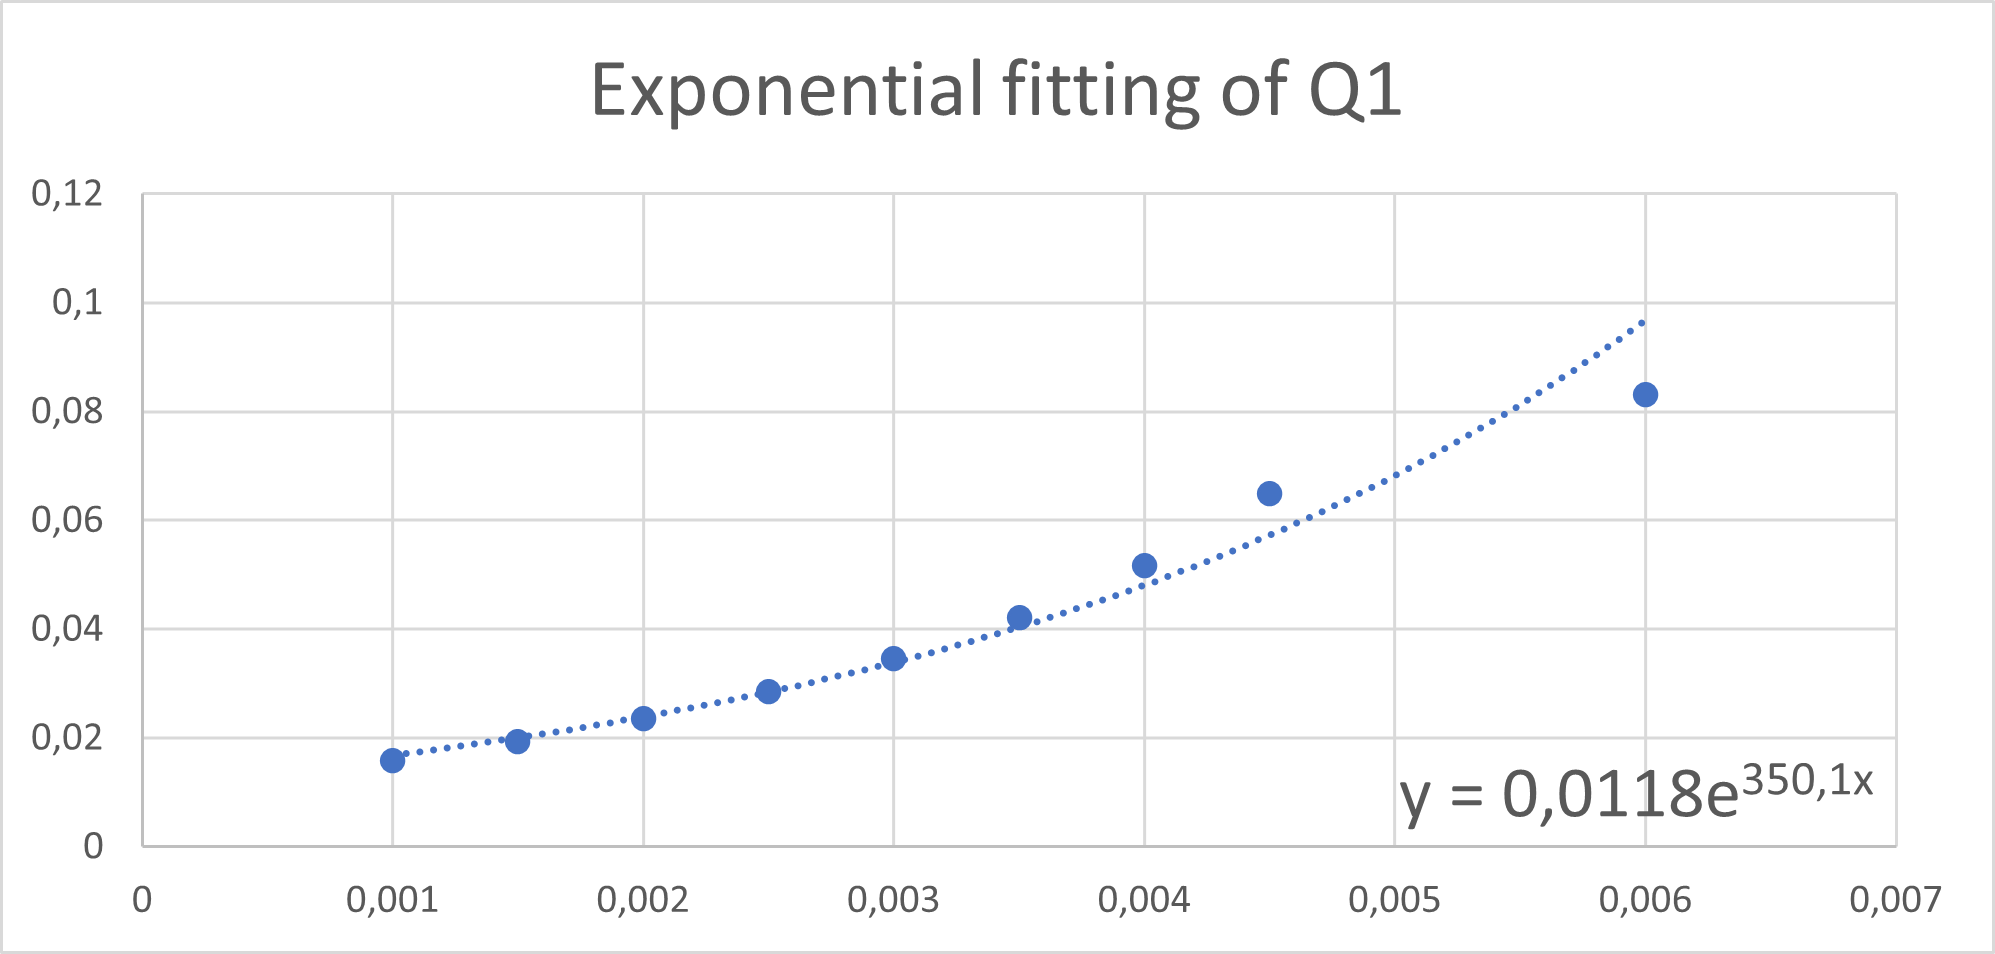
\includegraphics[width=\textwidth]{./data_analysis/Q05_exp_delta.png}
                            \caption{Fitting with the exponential}
                            \label{fig:Q05_exp_delta}
                        \end{minipage}
                        \hspace{10mm}
                        \begin{minipage}[c]{.40\textwidth}
                            \centering
                            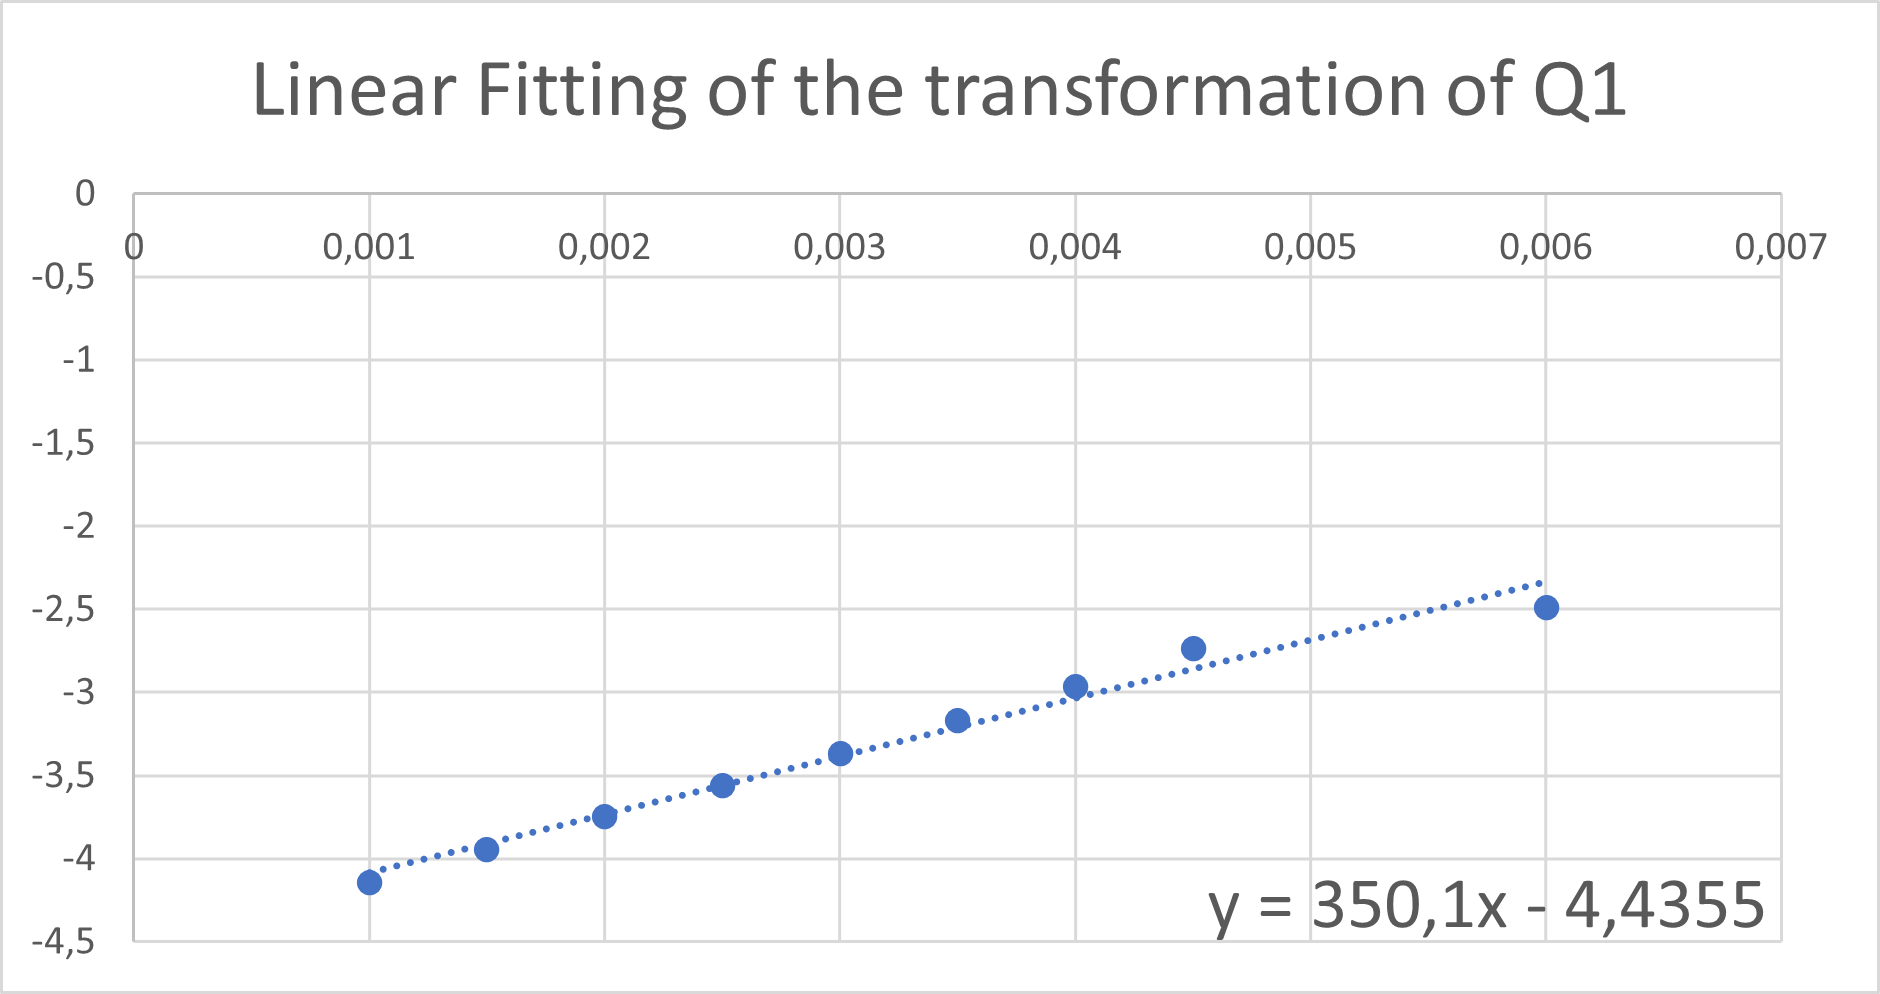
\includegraphics[width=\textwidth]{./data_analysis/Q05_lin_delta.png}
                            \caption{Transformation of the exponential for linear regression}
                            \label{fig:Q05_lin_delta}
                        \end{minipage}
                    \end{figure}
                    
                    \begin{table}[htbp]
                        \centering 
                        \begin{tabular}{|c|c|c|}
                            
                            \hline
                            \multicolumn{3}{|c|}{\bf Confidence interval with 95\% confidence level} \\
                            
                            \hline
                            \ & Slope & Offset\\
                            \hline
                            \ Upper Limit & 350.2274218 & -4.293371211 \\ 
                            \hline
                            \ Lower Limit & 349.9725782 & -4.577628789 \\ 
                            \hline
                        \end{tabular}
                        \label{table:CI_05_fitting}
                    \end{table}
    \newpage            
        \subsection{Case $Q = S_t$}
            Here what we achieved was that $\delta$ accounted for the $48,39\%$ of the variation and $\mu$ for the $33,3\%$. For this reason we decided to study two different cases, one in which we varied only the vacation and another one in which we varied only the service time.

            Moreover we noticed that the interplay between $\delta$ and $\mu$ accounted for the $6,87\%$, so we decided to study that case as well.
            
            \subsubsection{Linear regression for $\delta$}
                \paragraph{Settings for the simulations} \hfill \\
                    \lstinputlisting[language=Octave]{txt_ini/Q1_delta.txt}
                \paragraph{Fitting} \hfill \\

                    In Figure \ref{fig:Q1_exp_delta} is shown the scatterplot of the distribution obtained by varying the vacations and maintaining fixed the other factors, from the graph we can easily see that the distribution fits very well an exponential. 
                    This result means that in this scenario, \textbf{increasing the vacations really decreases the performances of the system in terms of response time} and it is explainable by the fact that since $Q$ is of the same order of magnitude of $\mu$ and $\mu$ is exponentially distributed, a big job could arrive (with a requested service time bigger than the value of $Q$), the server will have to go on vacation to build a bigger turn to serve it.\\
                    
                    The linear transformation used for linear regression is shown in Figure \ref{fig:Q1_lin_delta}.          
                    
                    \begin{figure}[htbp!]
                        \centering
                        \begin{minipage}[c]{.40\textwidth}
                            \centering
                            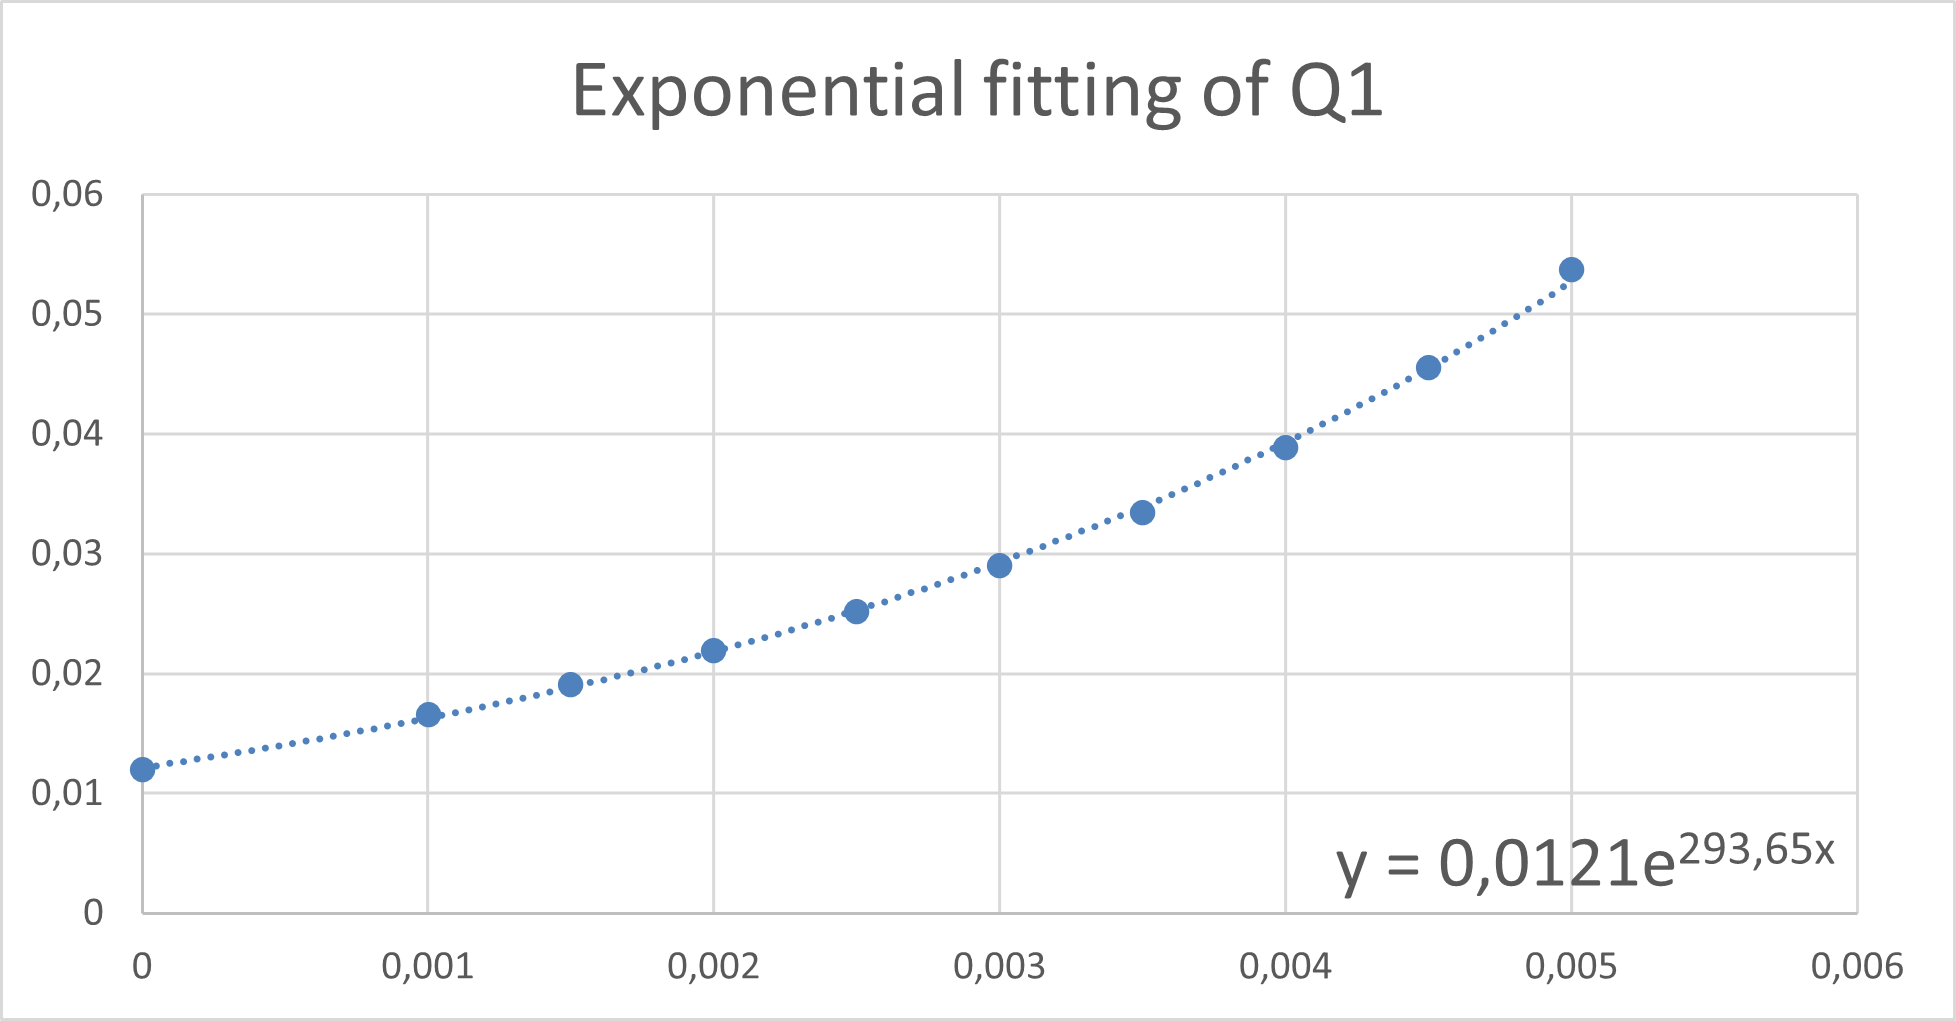
\includegraphics[width=\textwidth]{./data_analysis/Q1_exp_delta.png}
                            \caption{Fitting with the exponential}
                            \label{fig:Q1_exp_delta}
                        \end{minipage}
                        \hspace{10mm}
                        \begin{minipage}[c]{.40\textwidth}
                            \centering
                            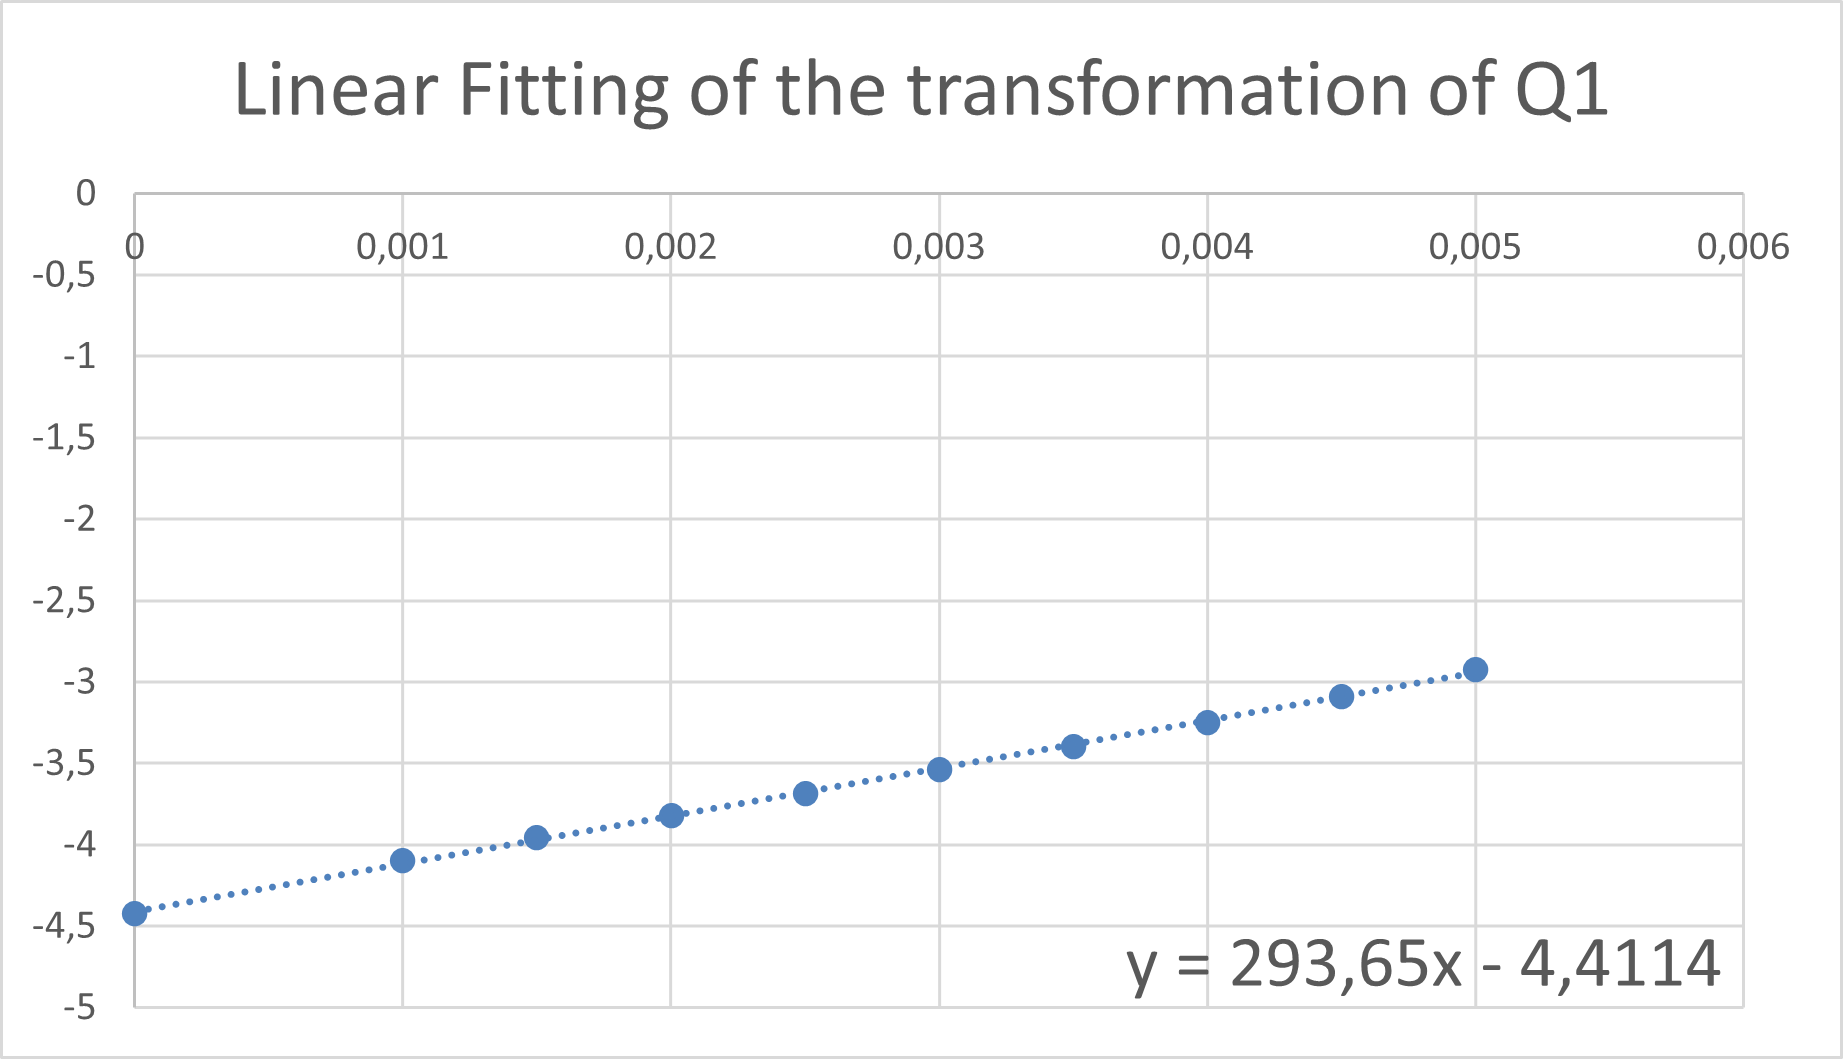
\includegraphics[width=\textwidth]{./data_analysis/Q1_lin_delta.png}
                            \caption{Transformation of the exponential for linear regression}
                            \label{fig:Q1_lin_delta}
                        \end{minipage}
                    \end{figure}
                    
                    \begin{table}[htbp]
                        \centering 
                        \begin{tabular}{|c|c|c|}
                            
                            \hline
                            \multicolumn{3}{|c|}{\bf Confidence interval with 95\% confidence level} \\
                            
                            \hline
                            \ & Slope & Offset\\
                            \hline
                            \ Upper Limit & 293.6720203 & -4.386202448 \\ 
                            \hline
                            \ Lower Limit & 293.6279797 & -4.436597552 \\ 
                            \hline
                        \end{tabular}
                        \label{table:CI_1_fitting_delta}
                    \end{table}
                    
            \subsubsection{Linear regression for $\mu$}
                \paragraph{Settings for the simulations} \hfill \\
                    \lstinputlisting[language=Octave]{txt_ini/Q1_mu.txt}
                \paragraph{Fitting} \hfill \\

                    Also in this case the model which fits the data in the best way is the exponential one (Figure \ref{fig:Q1_exp_mu}). This means that increasing the mean service time has a huge impact on the response time, which is reasonable if we think about how the system works.           
                    \begin{figure}[htbp!]
                        \centering
                        \begin{minipage}[c]{.40\textwidth}
                            \centering
                            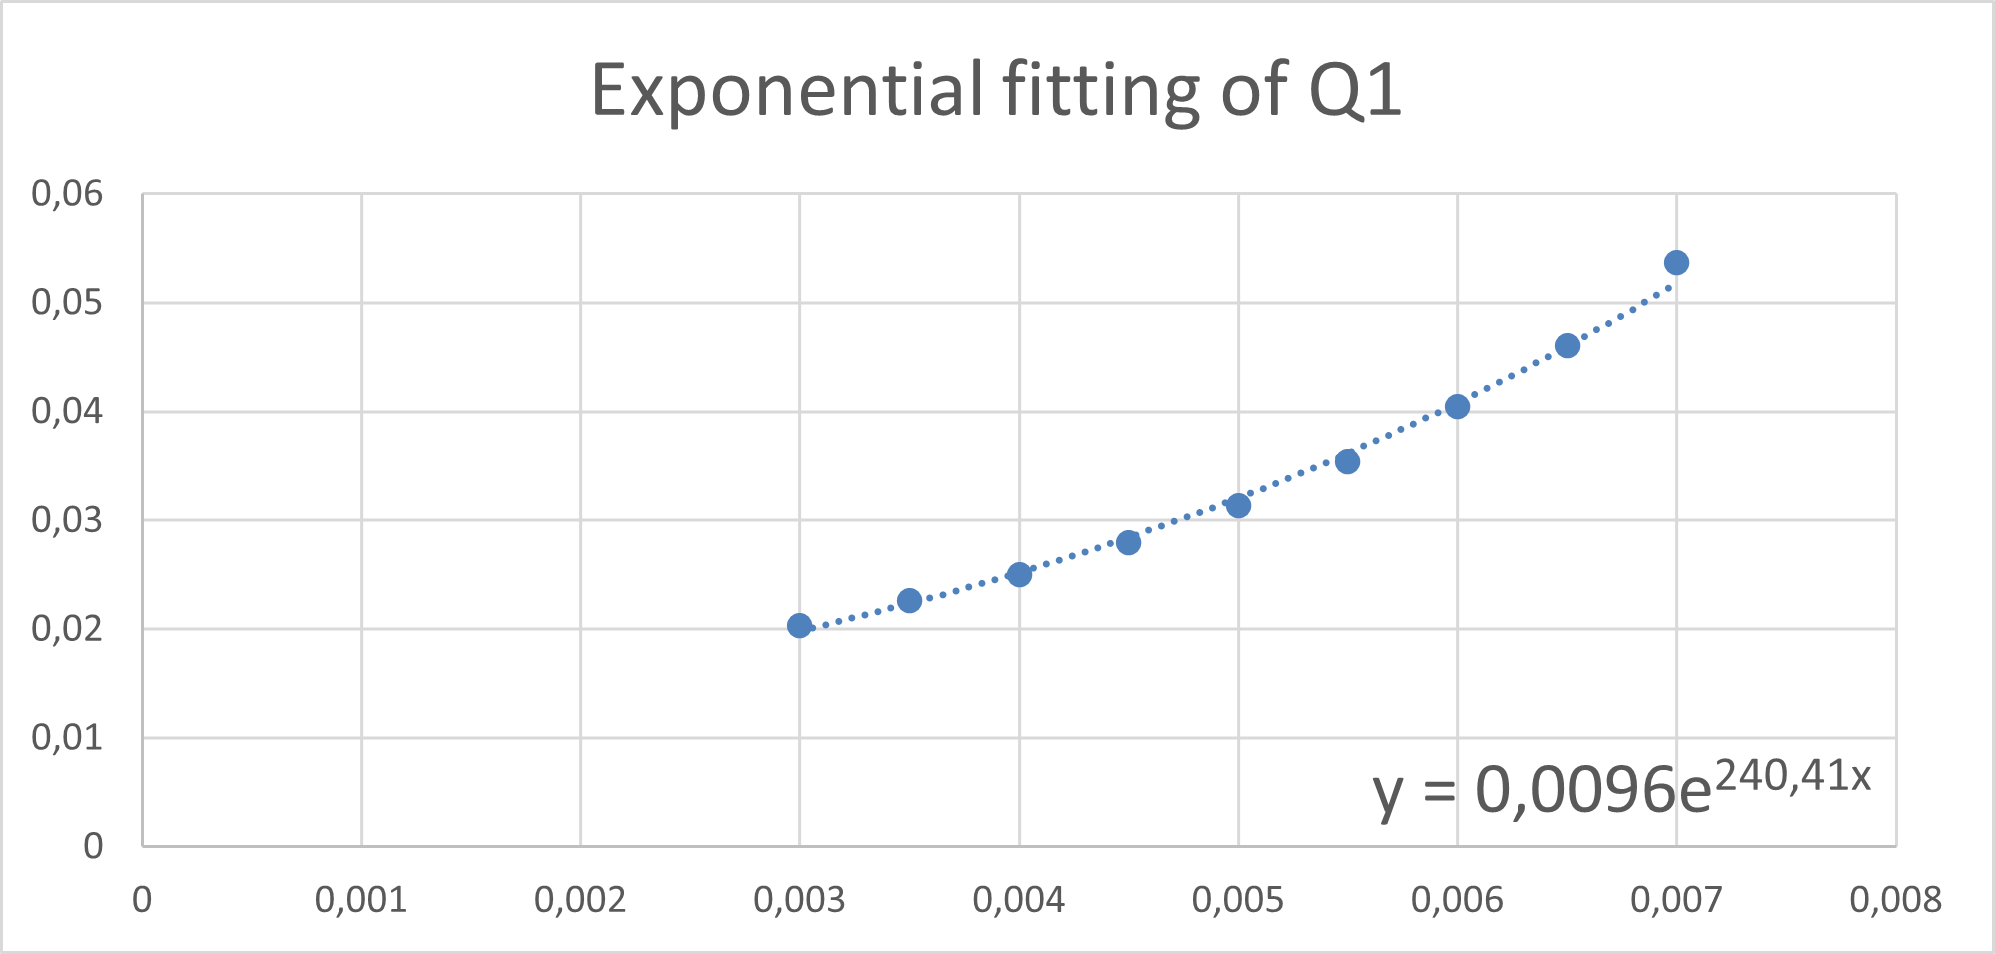
\includegraphics[width=\textwidth]{./data_analysis/Q1_exp_mu.png}
                            \caption{Fitting with the exponential}
                            \label{fig:Q1_exp_mu}
                        \end{minipage}
                        \hspace{10mm}
                        \begin{minipage}[c]{.40\textwidth}
                            \centering
                            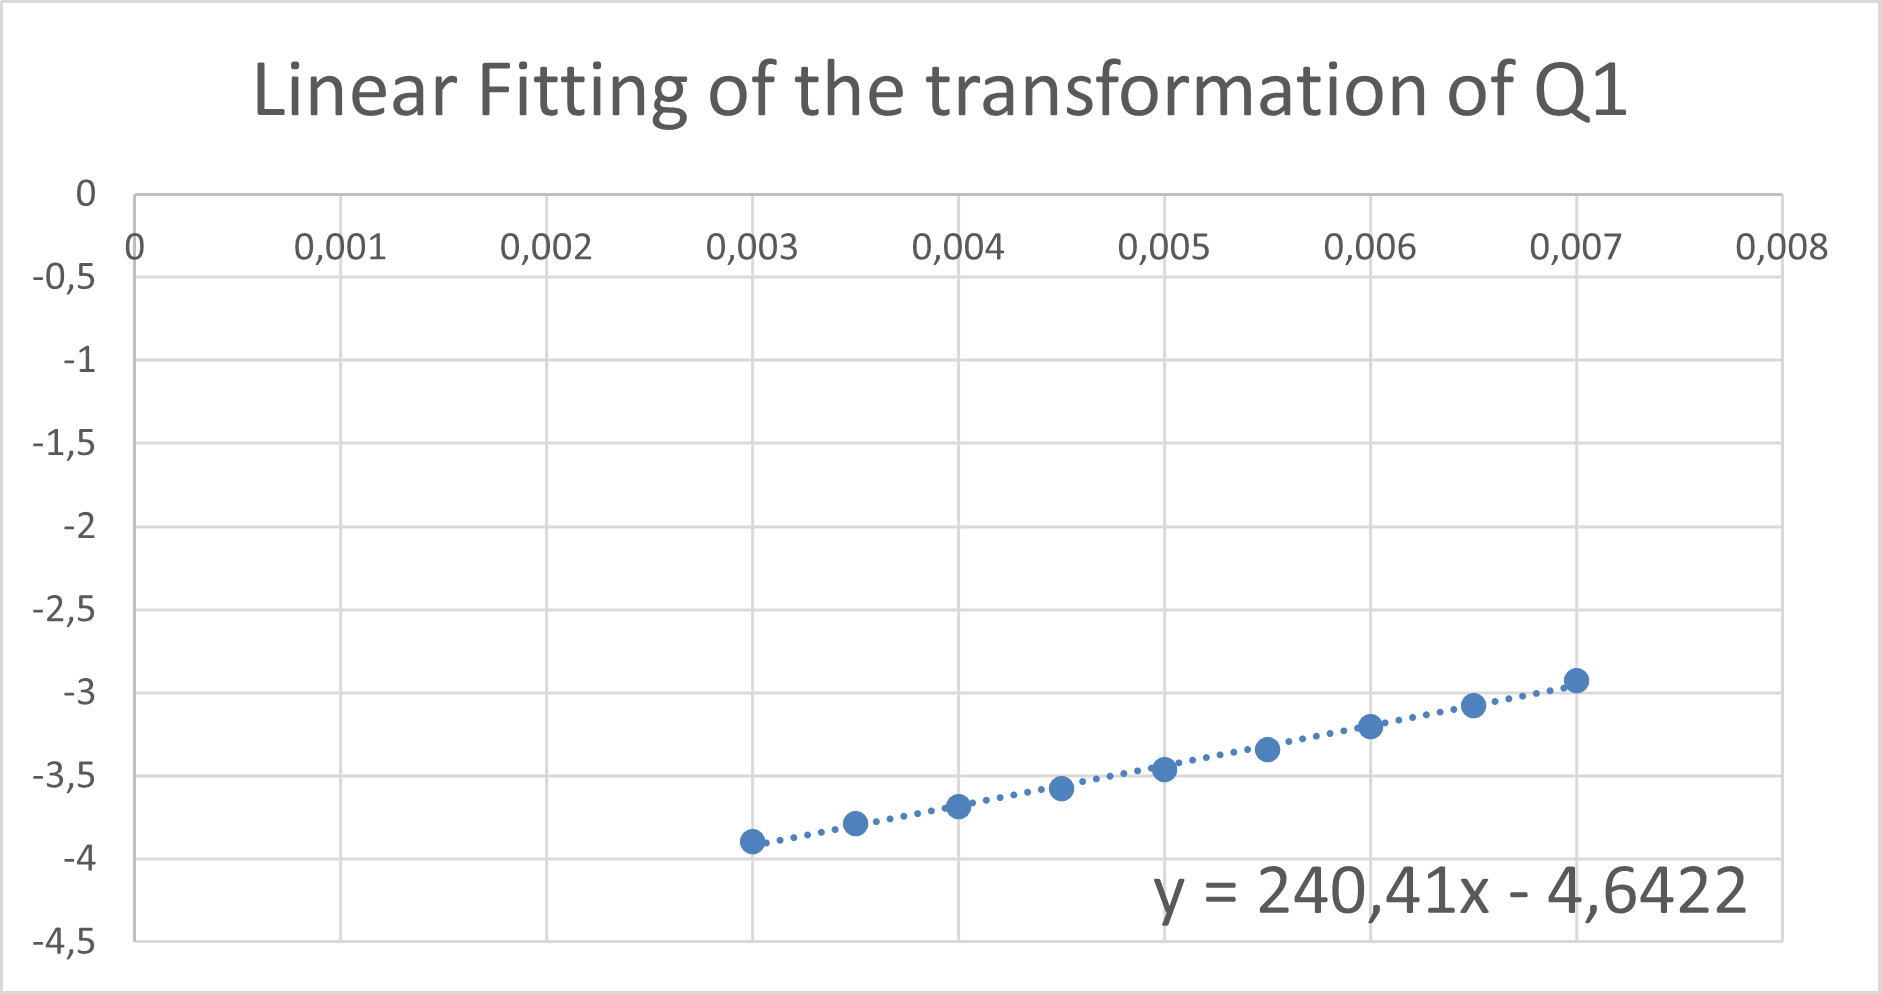
\includegraphics[width=\textwidth]{./data_analysis/Q1_lin_mu.png}
                            \caption{Transformation of the exponential for linear regression}
                            \label{fig:Q1_lin_mu}
                        \end{minipage}
                    \end{figure}
                    
                    \begin{table}[htbp]
                        \centering 
                        \begin{tabular}{|c|c|c|}
                            
                            \hline
                            \multicolumn{3}{|c|}{\bf Confidence interval with 95\% confidence level} \\
                            
                            \hline
                            \ & Slope & Offset\\
                            \hline
                            \ Upper Limit & 240.4648084 & -4.579350362 \\ 
                            \hline
                            \ Lower Limit & 240.3551916 & -4.705049638 \\ 
                            \hline
                        \end{tabular}
                        \label{table:CI_1_fitting_mu}
                    \end{table}
                    
            \subsubsection{Linear regression for $\delta \mu$}
                \paragraph{Settings for the simulations} \hfill \\
                    \lstinputlisting[language=Octave]{txt_ini/Q1_delta_mu.txt}
                \paragraph{Fitting} \hfill \\

                    Varying $\delta$ and $\mu$, the distribution of the mean response time for the scenario $Q = S_t$ fits very well an exponential (Figure \ref{fig:Q1_exp_delta_mu}), this result makes sense if we think that the mean response time has an exponential behavior depending on both $\delta$ and $\mu$. We decided to use as a variable for the linear regression the sum of $\delta$ and $\mu$, this because since the ration between the turn time and the service time is equal to 1, the time that the server actually needs to completely serve a job is, on average, the sum of the two.
                     
                    \begin{figure}[htbp!]
                        \centering
                        \begin{minipage}[c]{.40\textwidth}
                            \centering
                            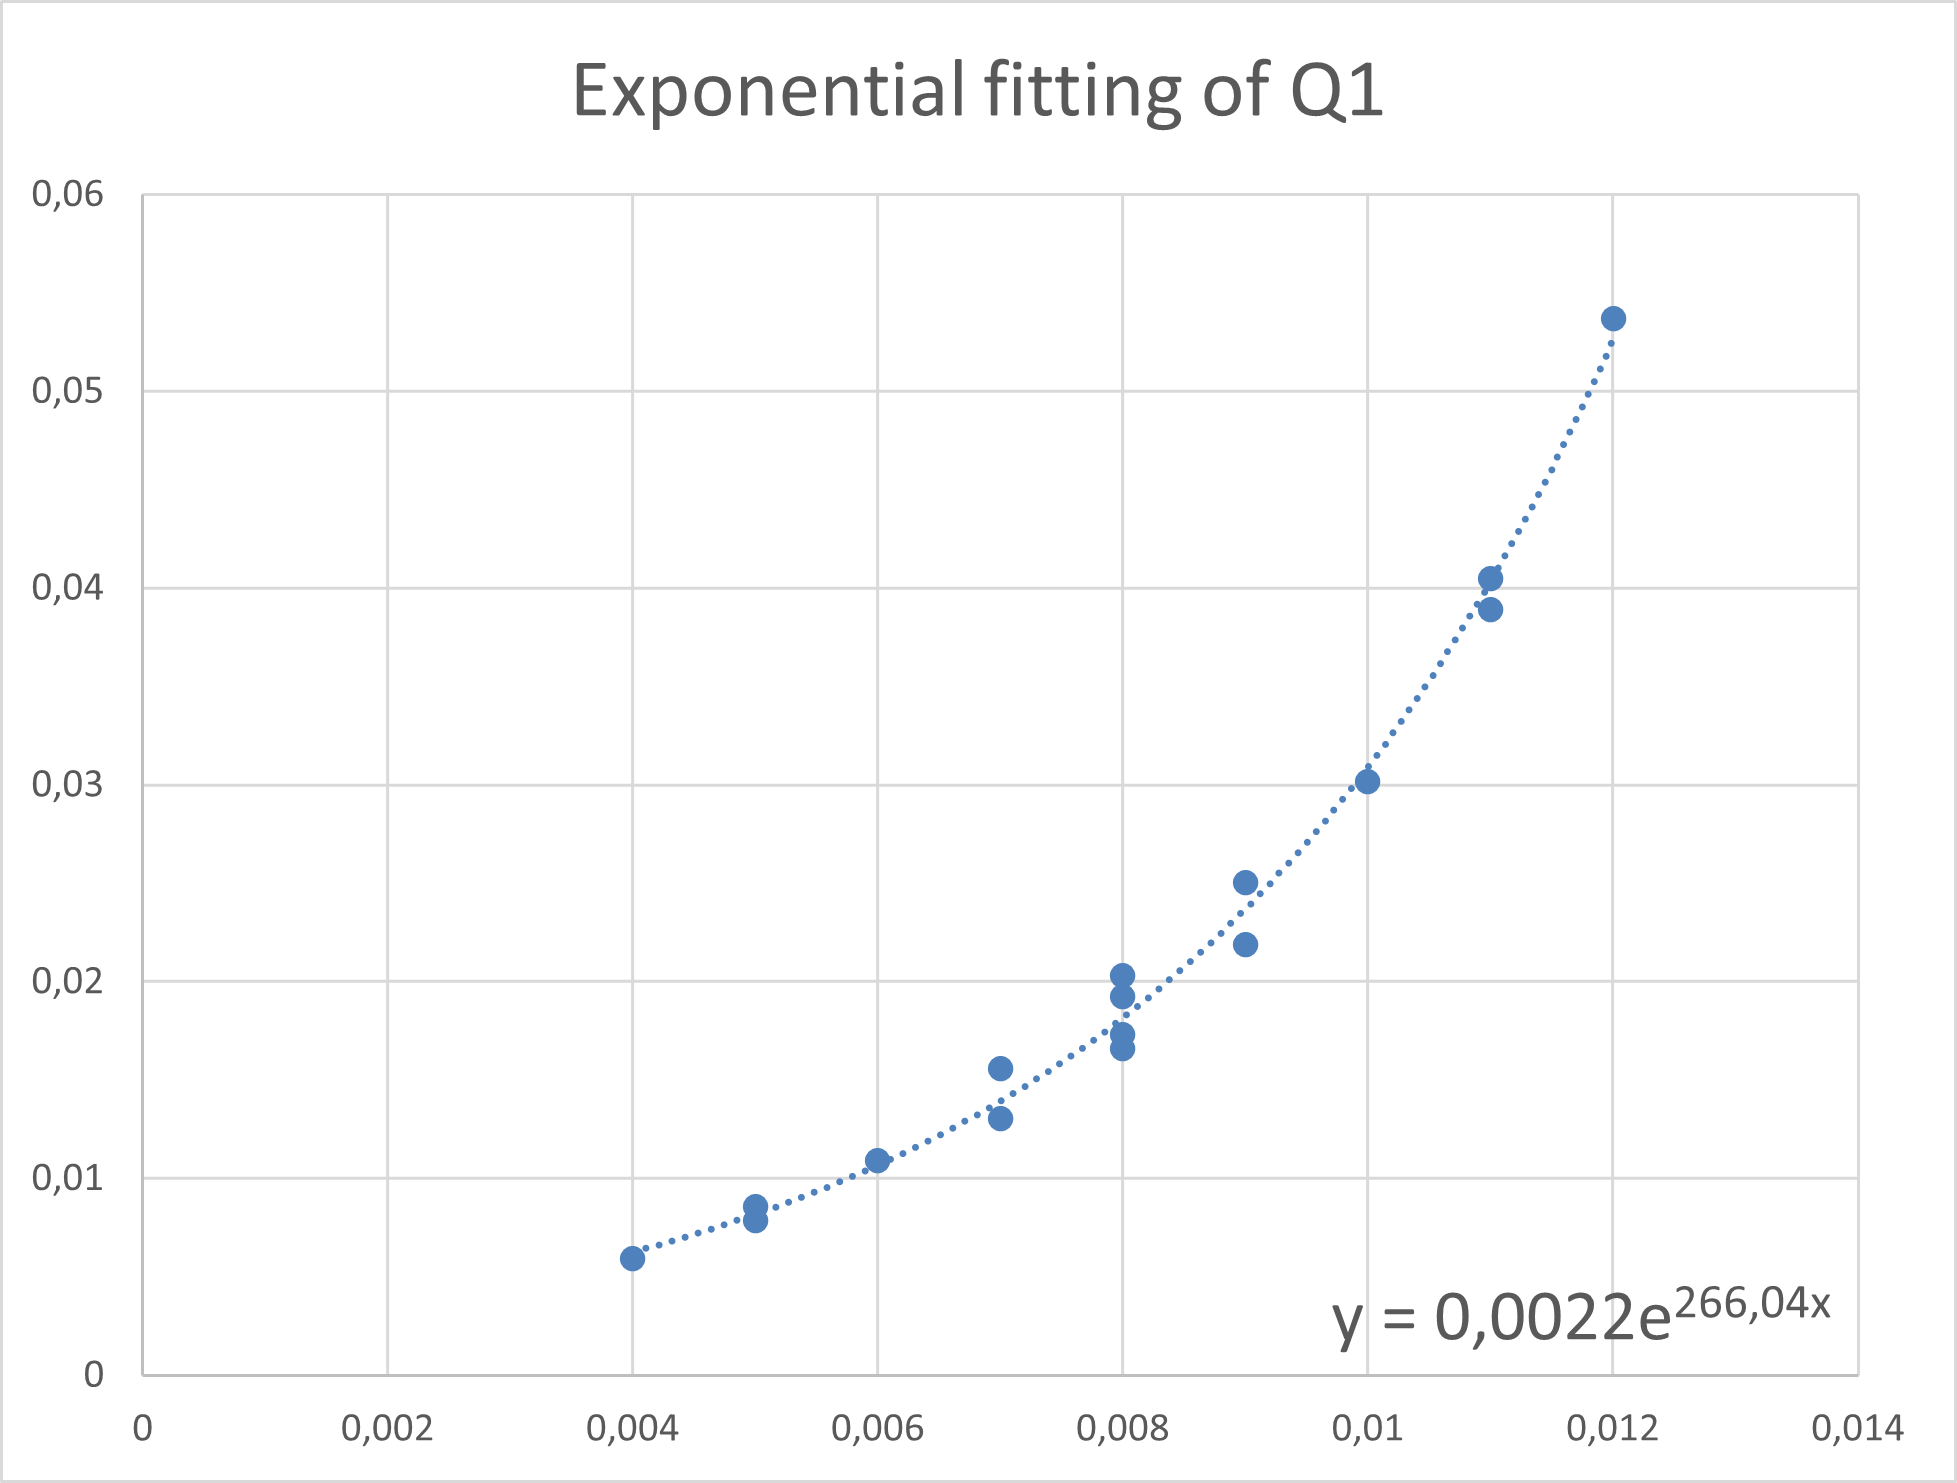
\includegraphics[width=\textwidth]{./data_analysis/Q1_exp_delta_mu.png}
                            \caption{Fitting with the exponential}
                            \label{fig:Q1_exp_delta_mu}
                        \end{minipage}
                        \hspace{10mm}
                        \begin{minipage}[c]{.40\textwidth}
                            \centering
                            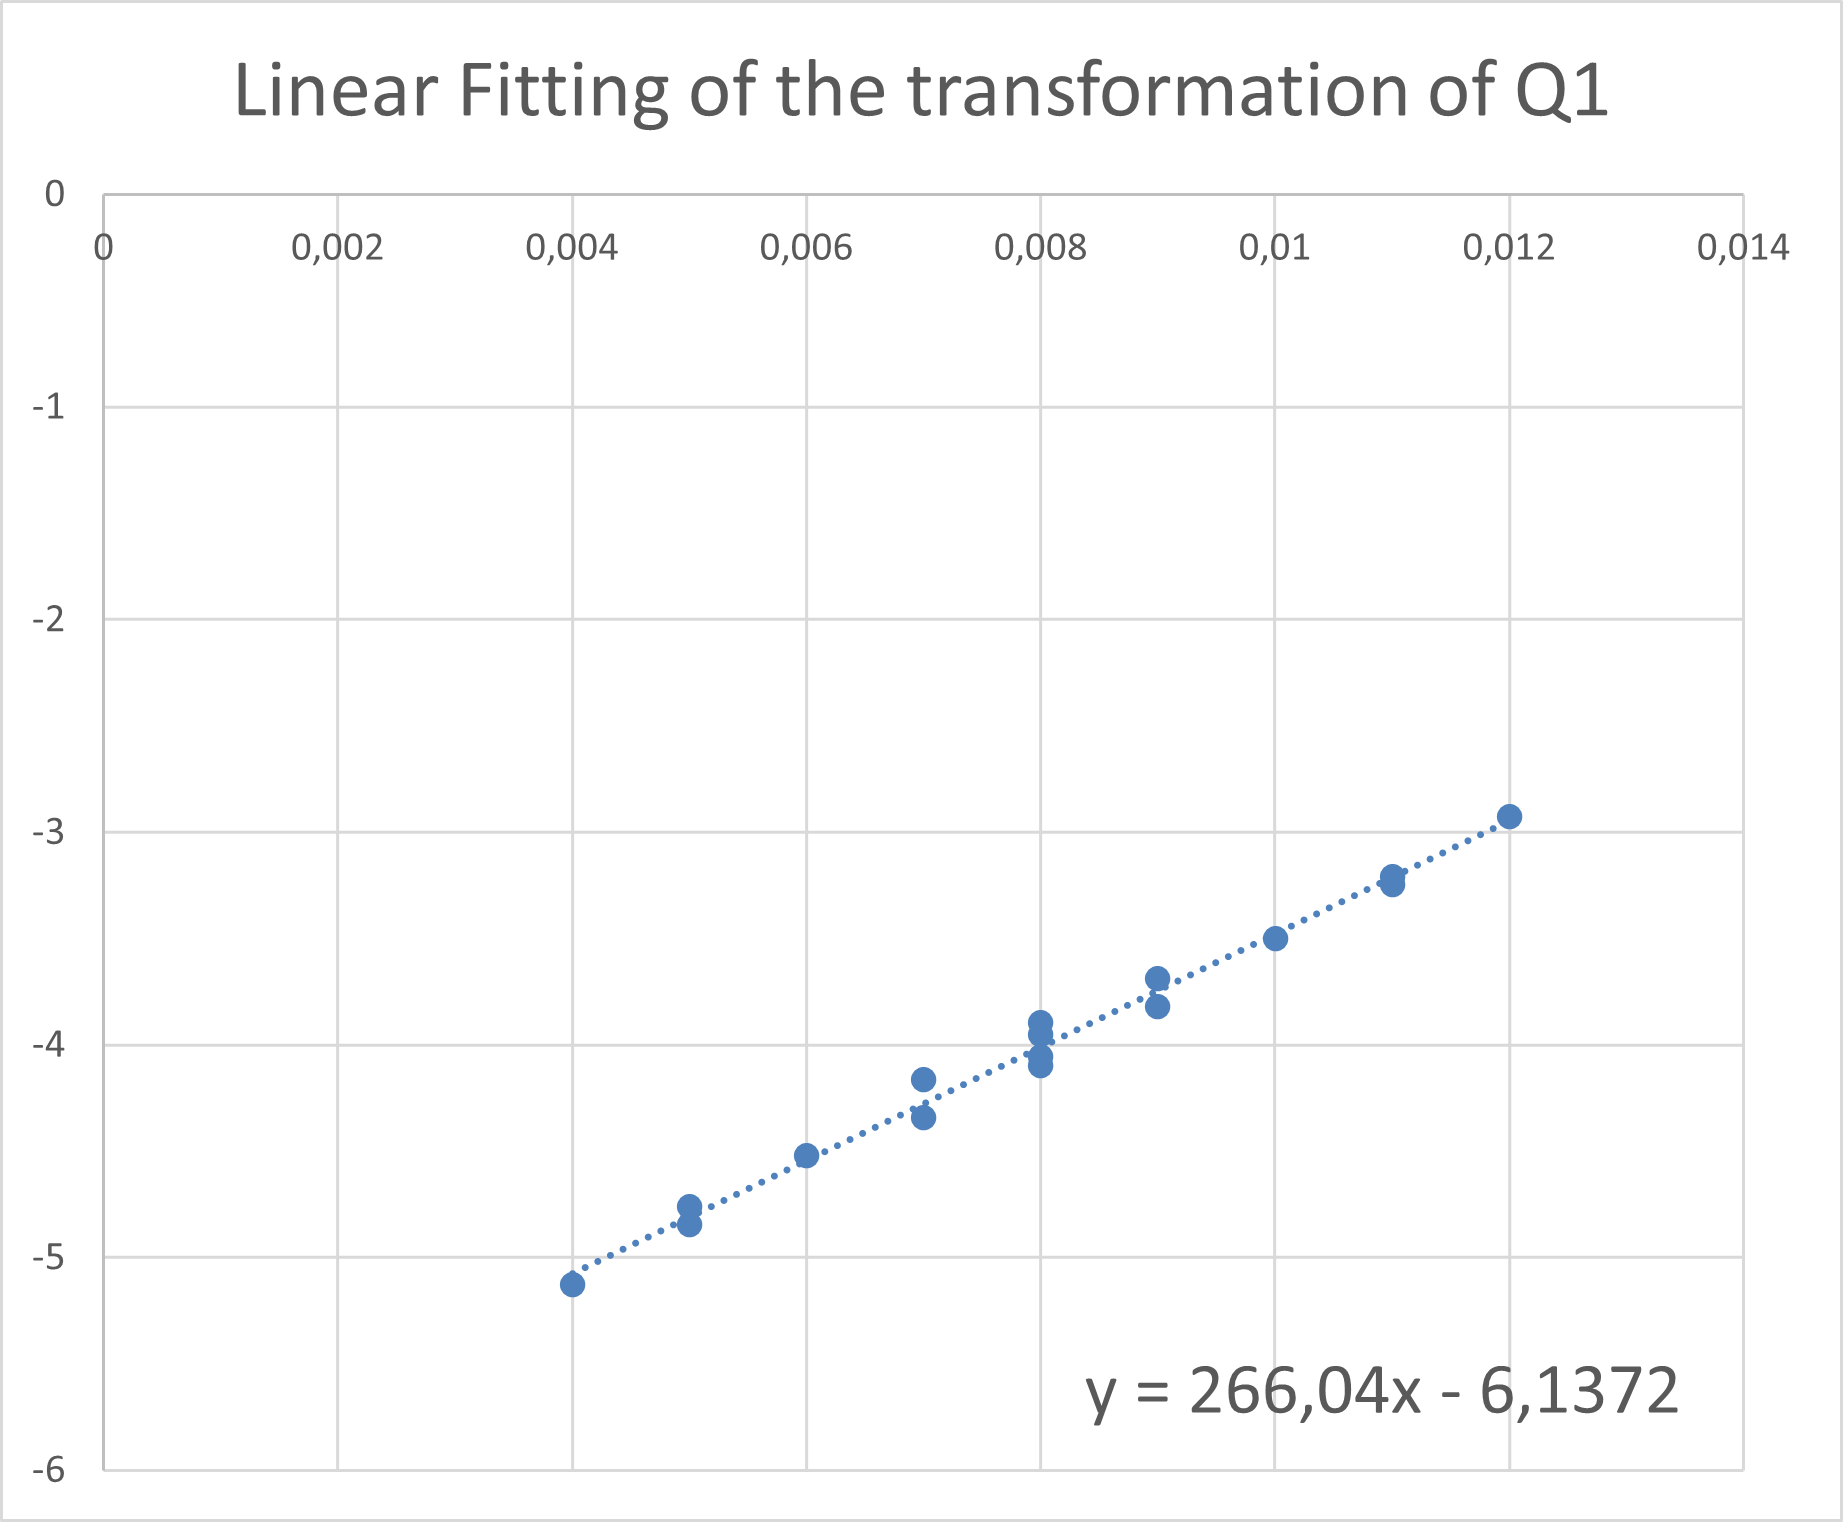
\includegraphics[width=\textwidth]{./data_analysis/Q1_lin_delta_mu.png}
                            \caption{Transformation of the exponential for linear regression}
                            \label{fig:Q1_lin_delta_mu}
                        \end{minipage}
                    \end{figure}
                    
                    \begin{table}[htbp!]
                        \centering 
                        \begin{tabular}{|c|c|c|}
                            
                            \hline
                            \multicolumn{3}{|c|}{\bf Confidence interval with 95\% confidence level} \\
                            
                            \hline
                            \ & Slope & Offset\\
                            \hline
                            \ Upper Limit & 266.0997927 & -6.077275135 \\ 
                            \hline
                            \ Lower Limit & 265.9802073 & -6.249309157 \\ 
                            \hline
                        \end{tabular}
                        \label{table:CI_1_fitting_delta-mu}
                    \end{table}
            
\newpage
        \subsection{Case $Q = 5S_t$}
            When we performed the data analysis for $Q = 5S_t$, we decided to study two cases in which we varied the most affecting factors discovered with the $2^k r$ factorial analysis that are the service time $\mu$ ($61.26\%$) and the interplay of the service time and the inter-arrivals ($10\%$). 
            
            \subsubsection{Linear regression for $\mu$}
                \paragraph{Settings for the simulations} \hfill \\
                    \lstinputlisting[language=Octave]{txt_ini/Q5_mu.txt}
                \paragraph{Fitting} \hfill \\

                     In this case, the exponential is the model that best fits the distribution of the mean response time (Figure \ref{fig:Q5_exp_mu}), it is reasonable if we think that $Q$ is approximately equal to $5$ times $\mu$ so the server can serve approximately $5$ jobs before it goes on vacation (the server completes approximately 5 jobs in a single turn) so the vacation doesn't affect too much the response time, as a consequence keeping fixed the inter-arrivals of the jobs and increasing the service times, will cause a big increase of the response time.
                    
                    \begin{figure}[htbp!]
                        \centering
                        \begin{minipage}[c]{.40\textwidth}
                            \centering
                            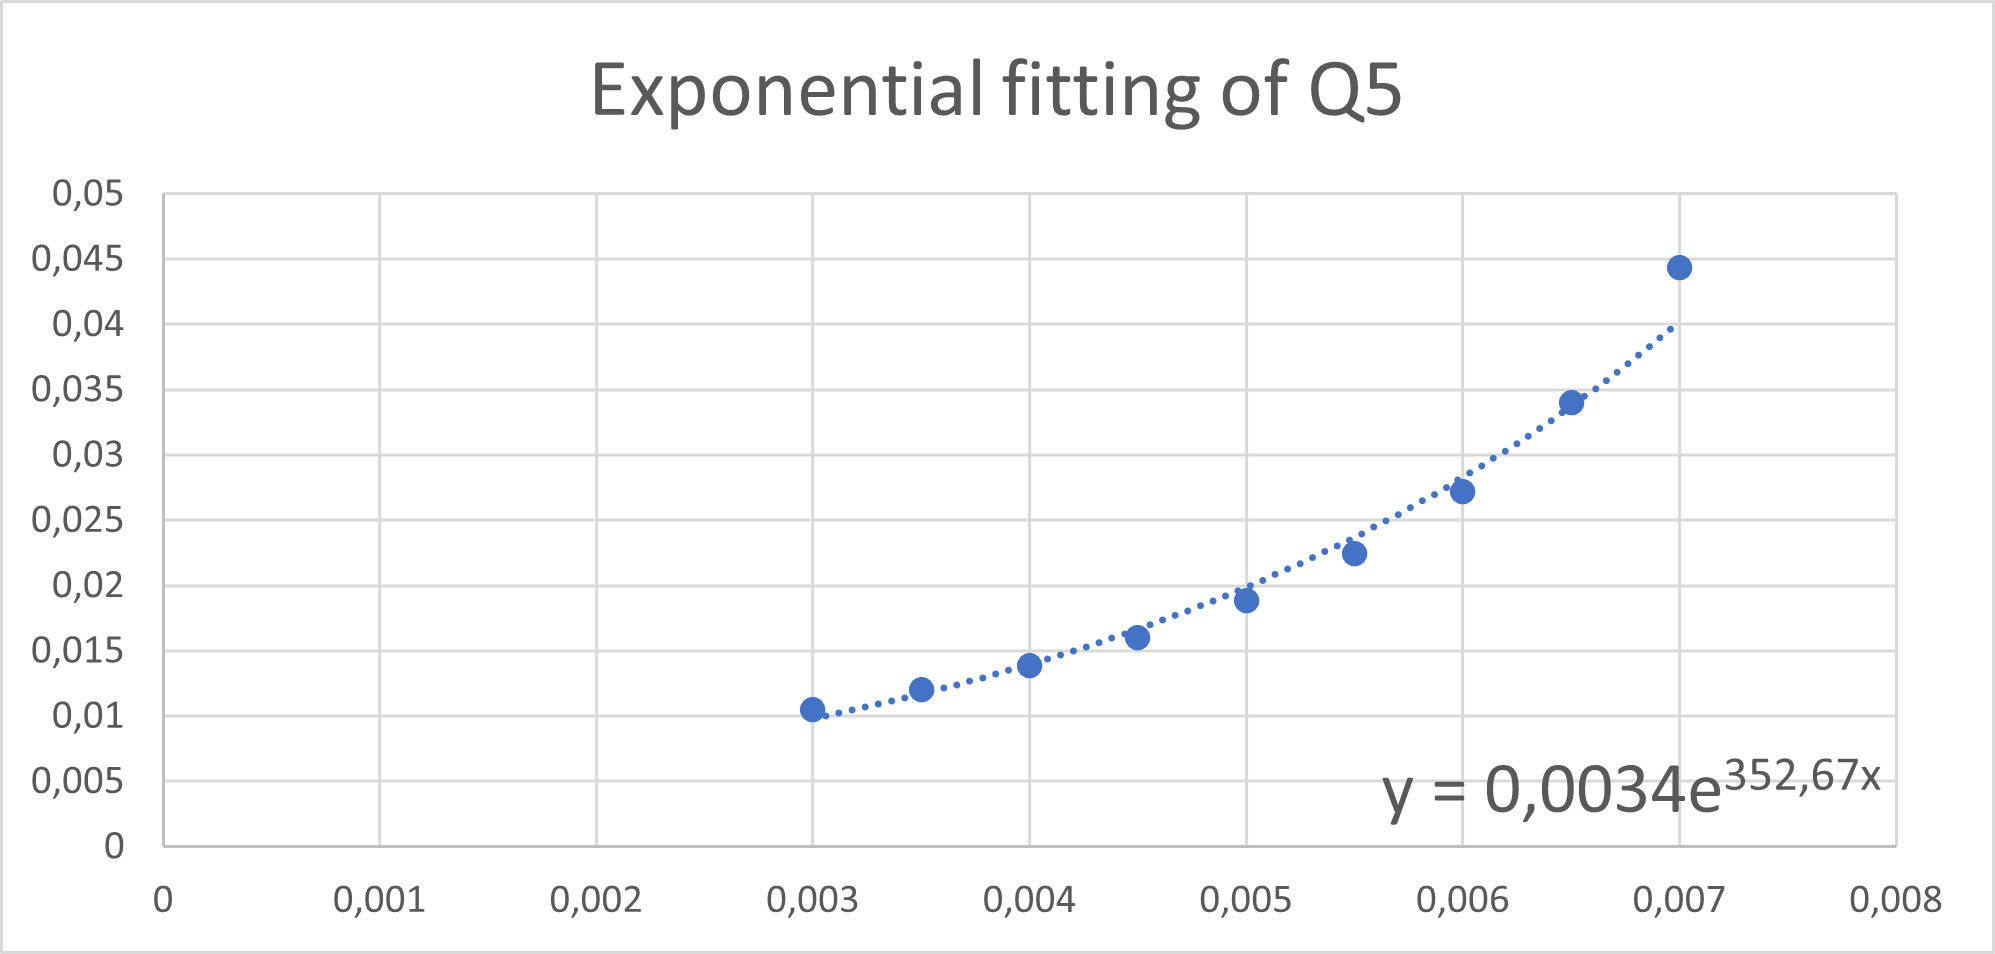
\includegraphics[width=\textwidth]{./data_analysis/Q5_exp_mu.png}
                            \caption{Fitting with the exponential}
                            \label{fig:Q5_exp_mu}
                        \end{minipage}
                        \hspace{10mm}
                        \begin{minipage}[c]{.40\textwidth}
                            \centering
                            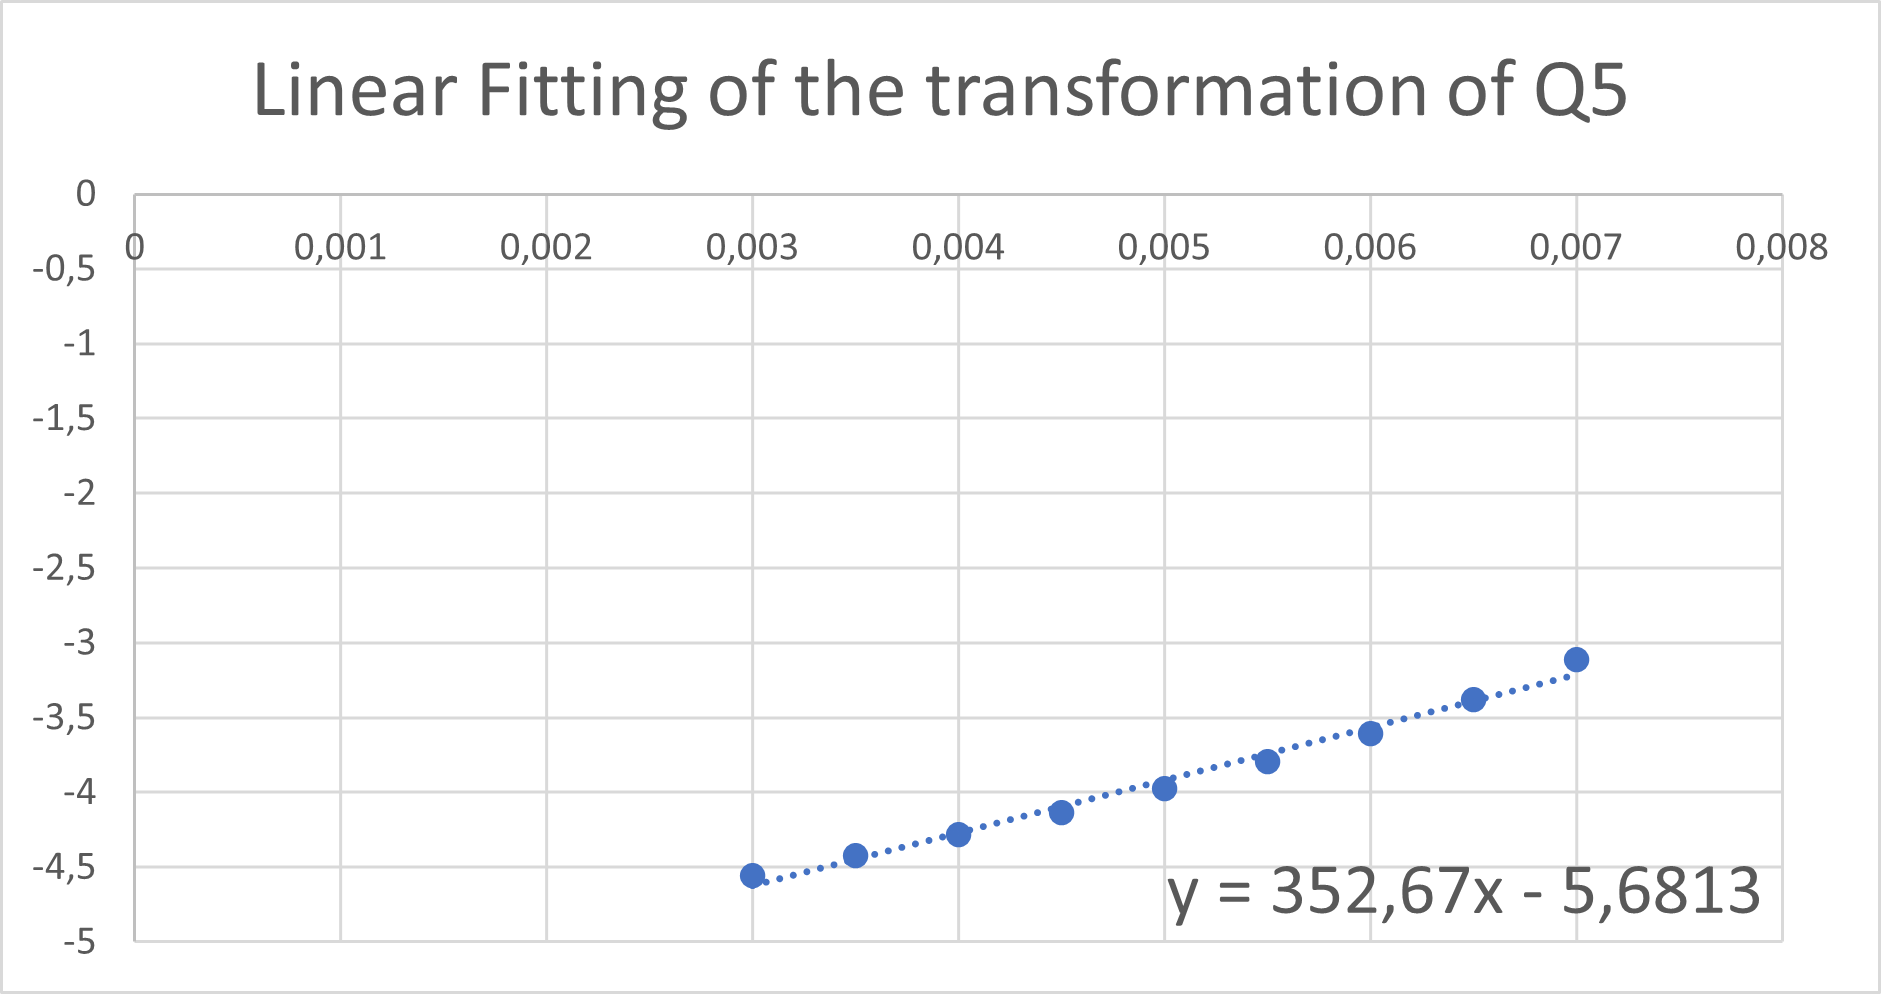
\includegraphics[width=\textwidth]{./data_analysis/Q5_lin_mu.png}
                            \caption{Transformation of the exponential for linear regression}
                            \label{fig:Q5_lin_mu}
                        \end{minipage}
                    \end{figure} 
                    
                    \begin{table}[htbp]
                        \centering 
                        \begin{tabular}{|c|c|c|}
                            
                            \hline
                            \multicolumn{3}{|c|}{\bf Confidence interval with 95\% confidence level} \\
                            
                            \hline
                            \ & Slope & Offset\\
                            \hline
                            \ Upper Limit & 352.7702998 & -5.550308268 \\ 
                            \hline
                            \ Lower Limit & 352.5697002 & -5.812291732 \\ 
                            \hline
                        \end{tabular}
                        \label{table:CI_5_fitting_mu}
                    \end{table}
                    
            \subsubsection{Linear regression for $\lambda \mu$}
                \paragraph{Settings for the simulations} \hfill \\
                    \lstinputlisting[language=Octave]{txt_ini/Q5_lambda_mu.txt}
                \paragraph{Fitting} \hfill \\
                    
                     We decided to study the interplay of the two factors as the ratio between the Inter-arrival \textit{rate} and the Service time \textit{rate},  because it resembles the utilization for an M/M/1 system. In fact, for big values of the ratio between Q and the service time our server behaves in such way. The response time increases exponentially with the utilization of the M/M/1, and the system does the same thing, as expected. 
                     
                    \begin{figure}[htbp!]
                        \centering
                        \begin{minipage}[c]{.40\textwidth}
                            \centering
                            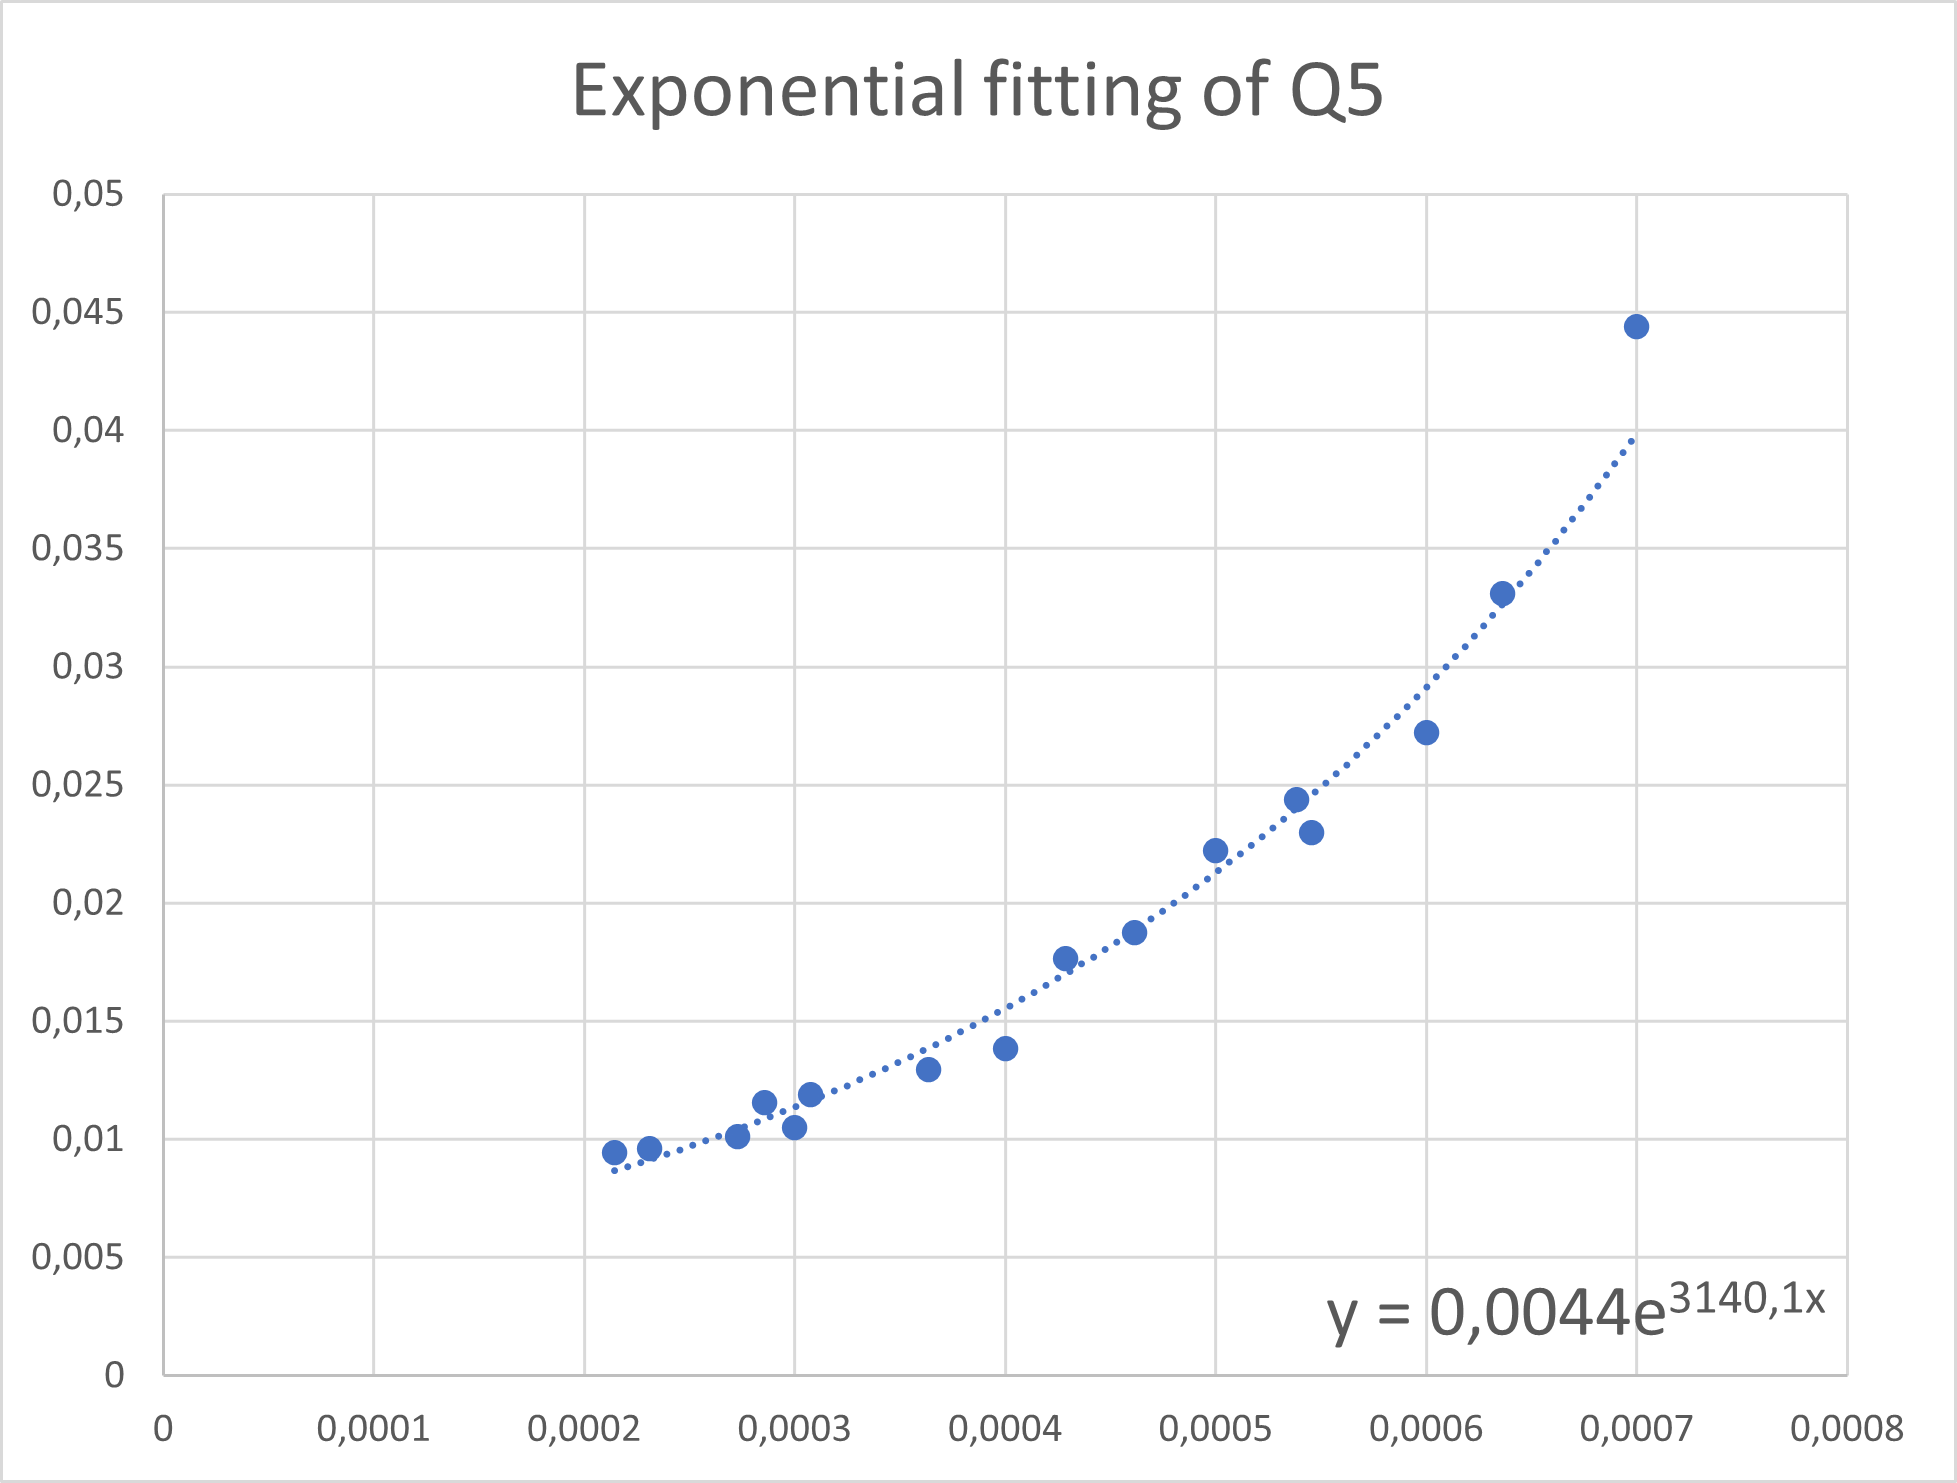
\includegraphics[width=\textwidth]{./data_analysis/Q5_exp_lambda_mu.png}
                            \caption{Fitting with the exponential}
                            \label{fig:Q5_exp_lambda_mu}
                        \end{minipage}
                        \hspace{10mm}
                        \begin{minipage}[c]{.40\textwidth}
                            \centering
                            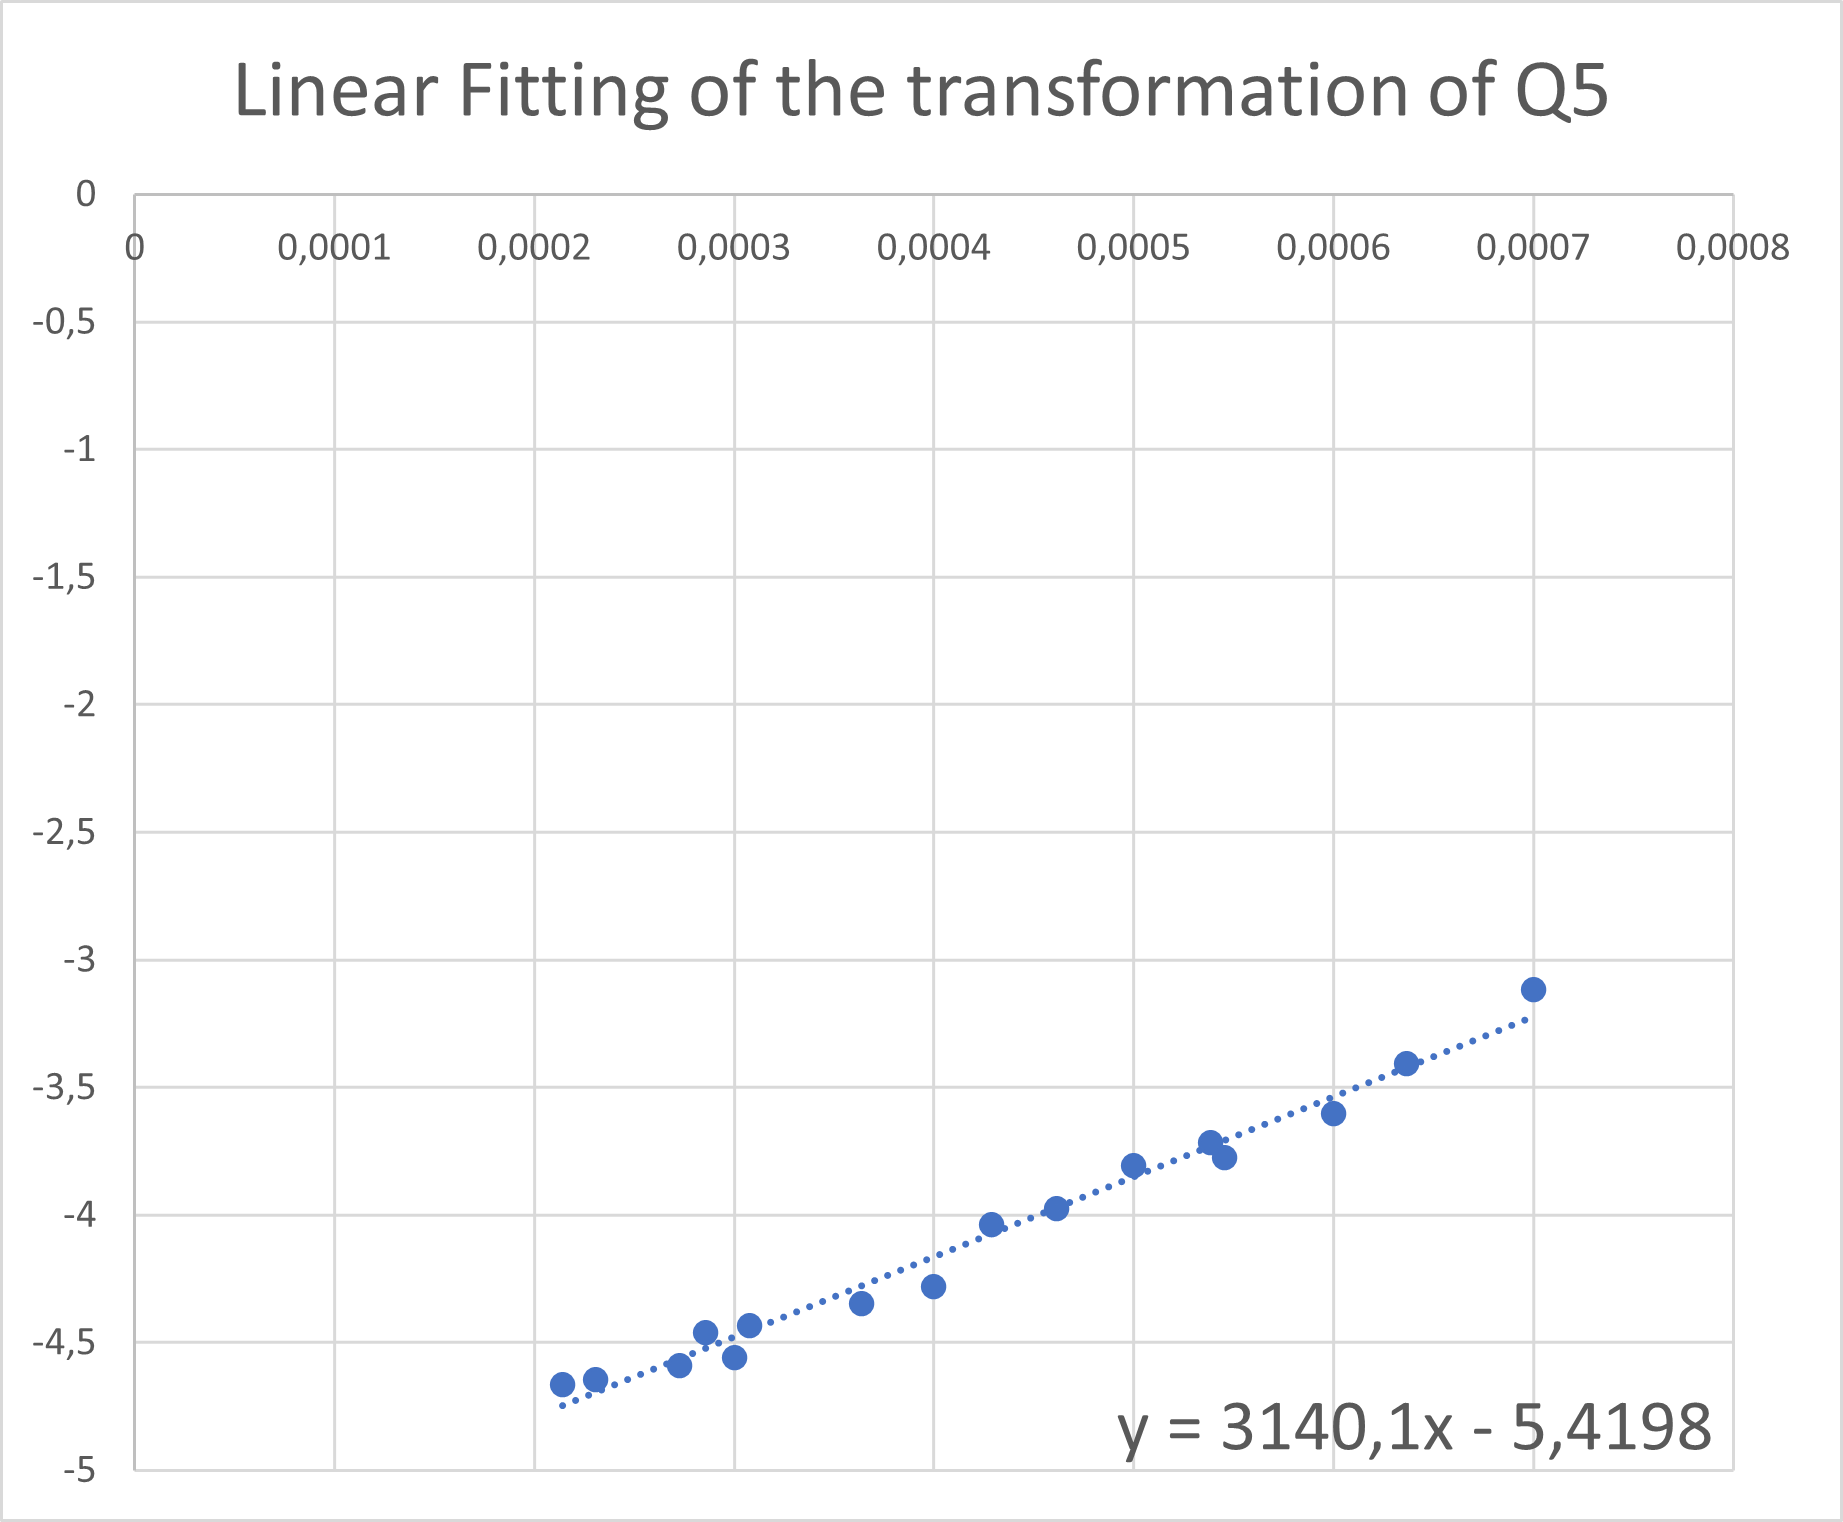
\includegraphics[width=\textwidth]{./data_analysis/Q5_lin_lambda_mu.png}
                            \caption{Transformation of the exponential for linear regression}
                            \label{fig:Q5_lin_lambda_mu}
                        \end{minipage}
                    \end{figure} 
                    
                    \begin{table}[htbp]
                        \centering 
                        \begin{tabular}{|c|c|c|}
                            
                            \hline
                            \multicolumn{3}{|c|}{\bf Confidence interval with 95\% confidence level} \\
                            
                            \hline
                            \ & Slope & Offset\\
                            \hline
                            \ Upper Limit & 3140.177707 & -5.340380178 \\ 
                            \hline
                            \ Lower Limit & 3140.022293 & -5.568380882 \\ 
                            \hline
                        \end{tabular}
                        \label{table:CI_5_fitting_lambda}
                    \end{table}
                
 \newpage               
        \subsection{Case $Q = 10S_t$}
            For $Q = 10S_t$, the most affecting factors on the performance of the systems are the service time $\mu$ ($62.25\%$ of variation), the inter-arrivals of the jobs ($15.96\%$ of variation) $\lambda$ and the interplay of the two ($13.96\%$), so during the data analysis of this case, we decided to study just the effects of those factors in the three cases documented below.
            
            \subsubsection{Linear regression for $\mu$}
                \paragraph{Settings for the simulations} \hfill \\
                    \lstinputlisting[language=Octave]{txt_ini/Q10_mu.txt}
                \paragraph{Fitting} \hfill \\

                    Also in this case we used an exponential model to fit our data (Figure \ref{fig:Q10_exp_mu}). The response time grows exponentially with the value of service time for the same reasons explained in the case $Q = 5S_t$ where we varied the factor $\mu$ and we maintained fixed $\lambda$ and $\delta$.        
                    
                    \begin{figure}[htbp!]
                        \centering
                        \begin{minipage}[c]{.40\textwidth}
                            \centering
                            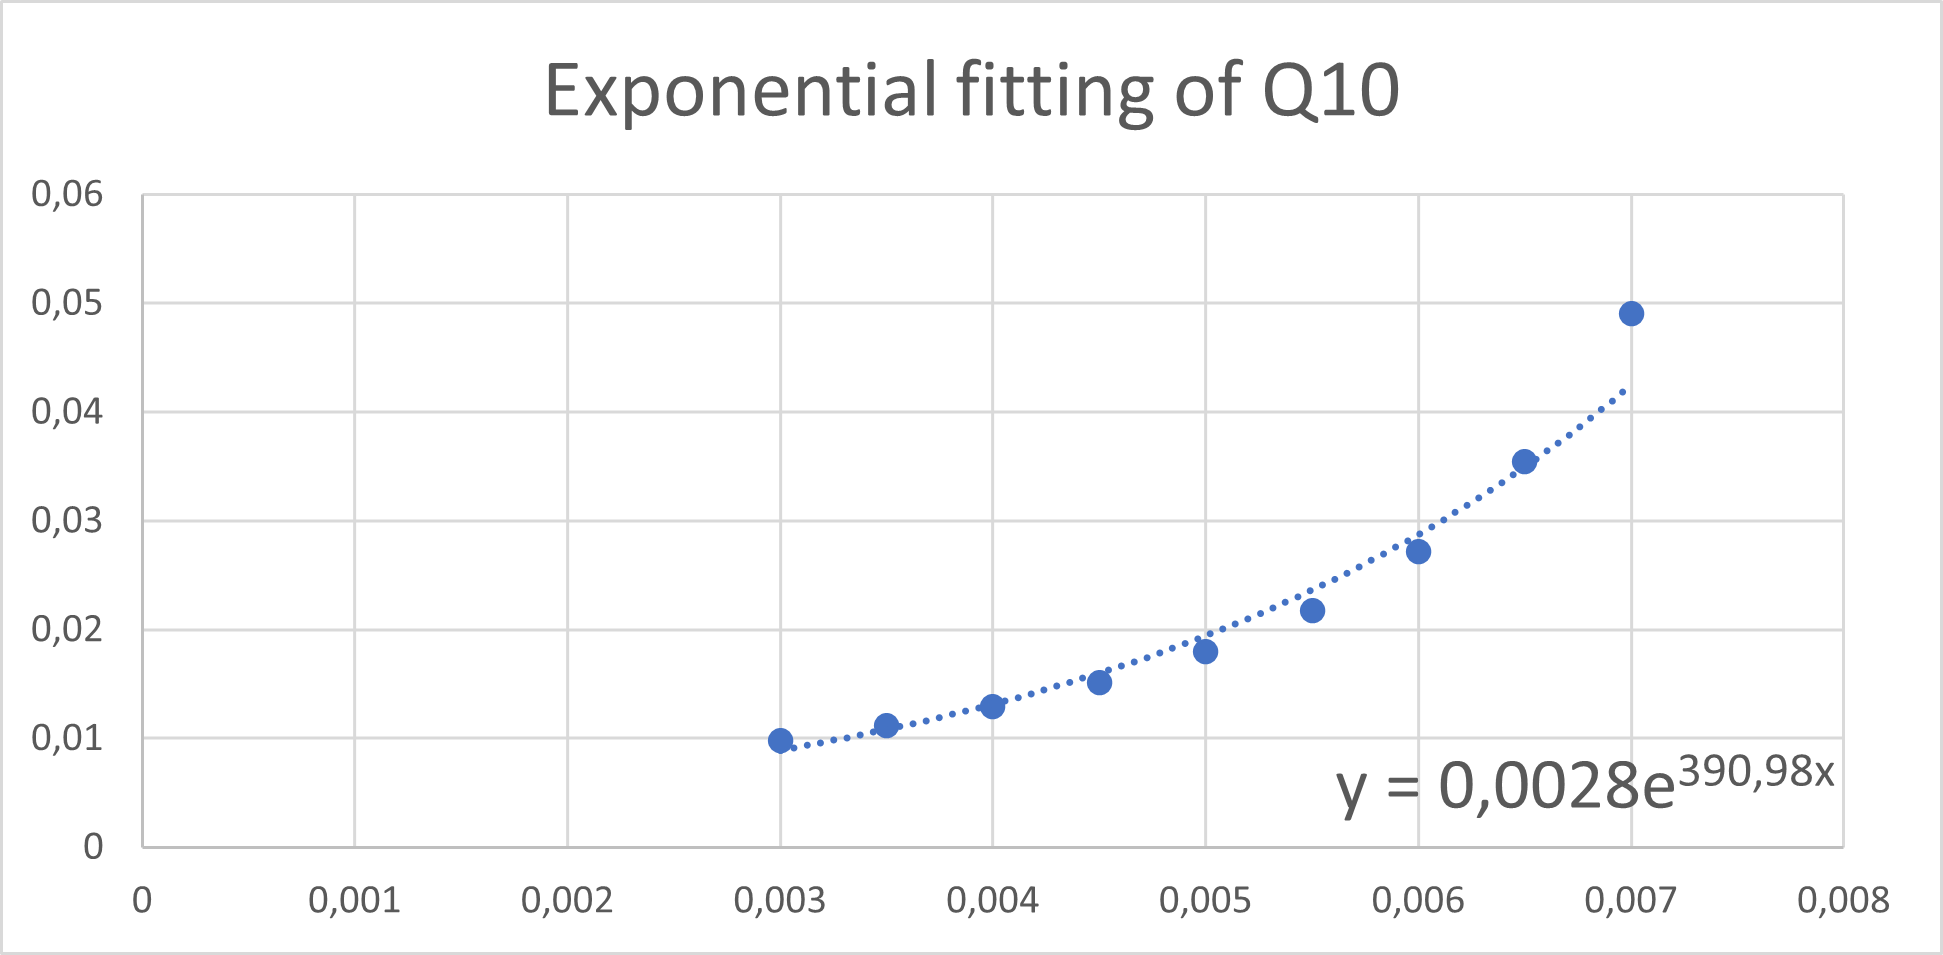
\includegraphics[width=\textwidth]{./data_analysis/Q10_exp_mu.png}
                            \caption{Fitting with the exponential.}
                            \label{fig:Q10_exp_mu}
                        \end{minipage}
                        \hspace{10mm}
                        \begin{minipage}[c]{.40\textwidth}
                            \centering
                            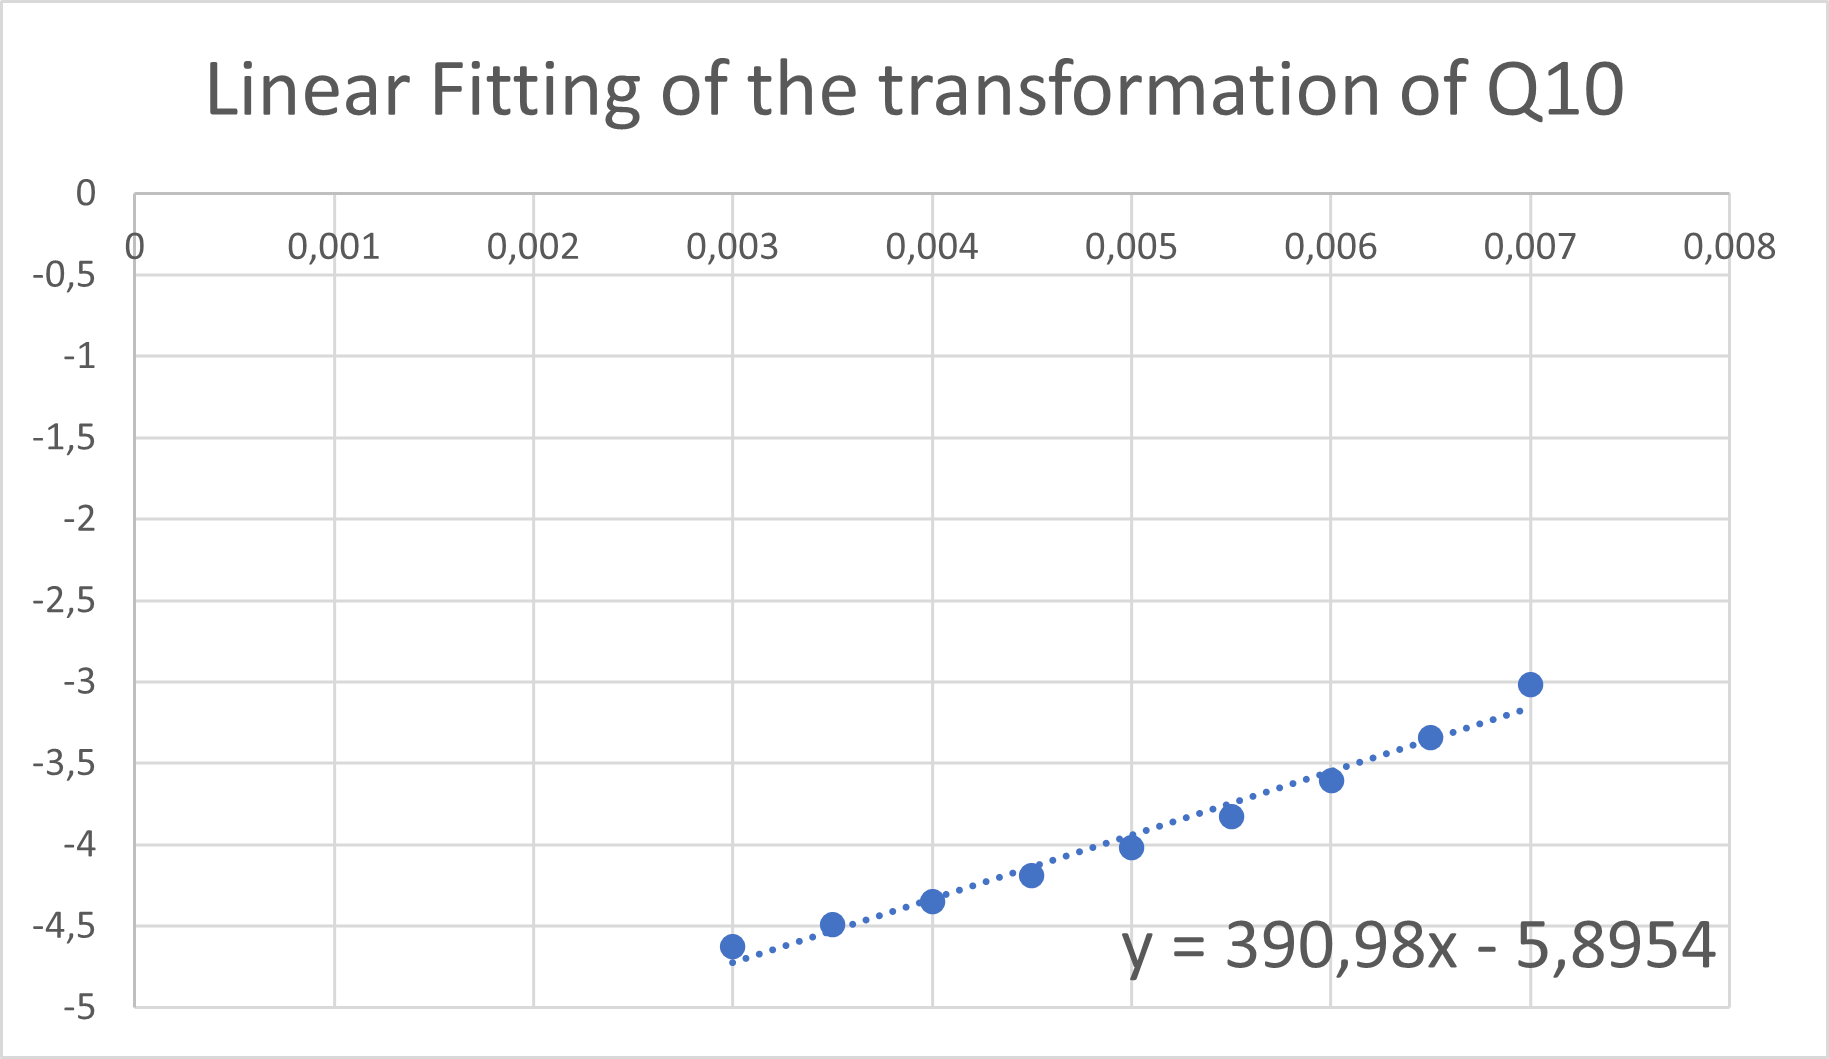
\includegraphics[width=\textwidth]{./data_analysis/Q10_lin_mu.png}
                            \caption{Transformation of the exponential for linear regression}
                            \label{fig:Q10_lin_mu}
                        \end{minipage}
                    \end{figure}
                    
                    \begin{table}[htbp]
                        \centering 
                        \begin{tabular}{|c|c|c|}
                            
                            \hline
                            \multicolumn{3}{|c|}{\bf Confidence interval with 95\% confidence level} \\
                            
                            \hline
                            \ & Slope & Offset\\
                            \hline
                            \ Upper Limit & 391.1127699 & -5.721008807 \\ 
                            \hline
                            \ Lower Limit & 390.8472301 & -6.069791193 \\ 
                            \hline
                        \end{tabular}
                        \label{table:CI_10_fitting_mu}
                    \end{table}
            
            \subsubsection{Linear regression for $\lambda$}
                \paragraph{Settings for the simulations} \hfill \\
                    \lstinputlisting[language=Octave]{txt_ini/Q10_lambda.txt}
                \paragraph{Fitting} \hfill \\

                    As we can see from Figure \ref{fig:Q10_exp_lambda}, we used an exponential to model the distribution of the response time even in this case. The practical explanation is that even if $Q$ is very big compared to the service time, if the inter-arrivals of the jobs are very frequent then the jobs may queue up and the response time grows, if instead the arrivals are not so close between each other, then the server can easily serve the jobs with a small response time. 
                    Note that this model works properly only inside the range of our interest. In fact, assuming that we take a very large value for $\lambda$, in this model the response time approaches $0$, but that doesn't make sense in the real system where the mean response time is lower bounded by a value depending on the actual service time and vacation period, also $\lambda$ can't be too small because of of the limit that we found for the constant case: 
                    $\lambda \ge \delta \frac{\mu}{Q} + \mu$.
                    
                    \begin{figure}[htbp!]
                        \centering
                        \begin{minipage}[c]{.40\textwidth}
                            \centering
                            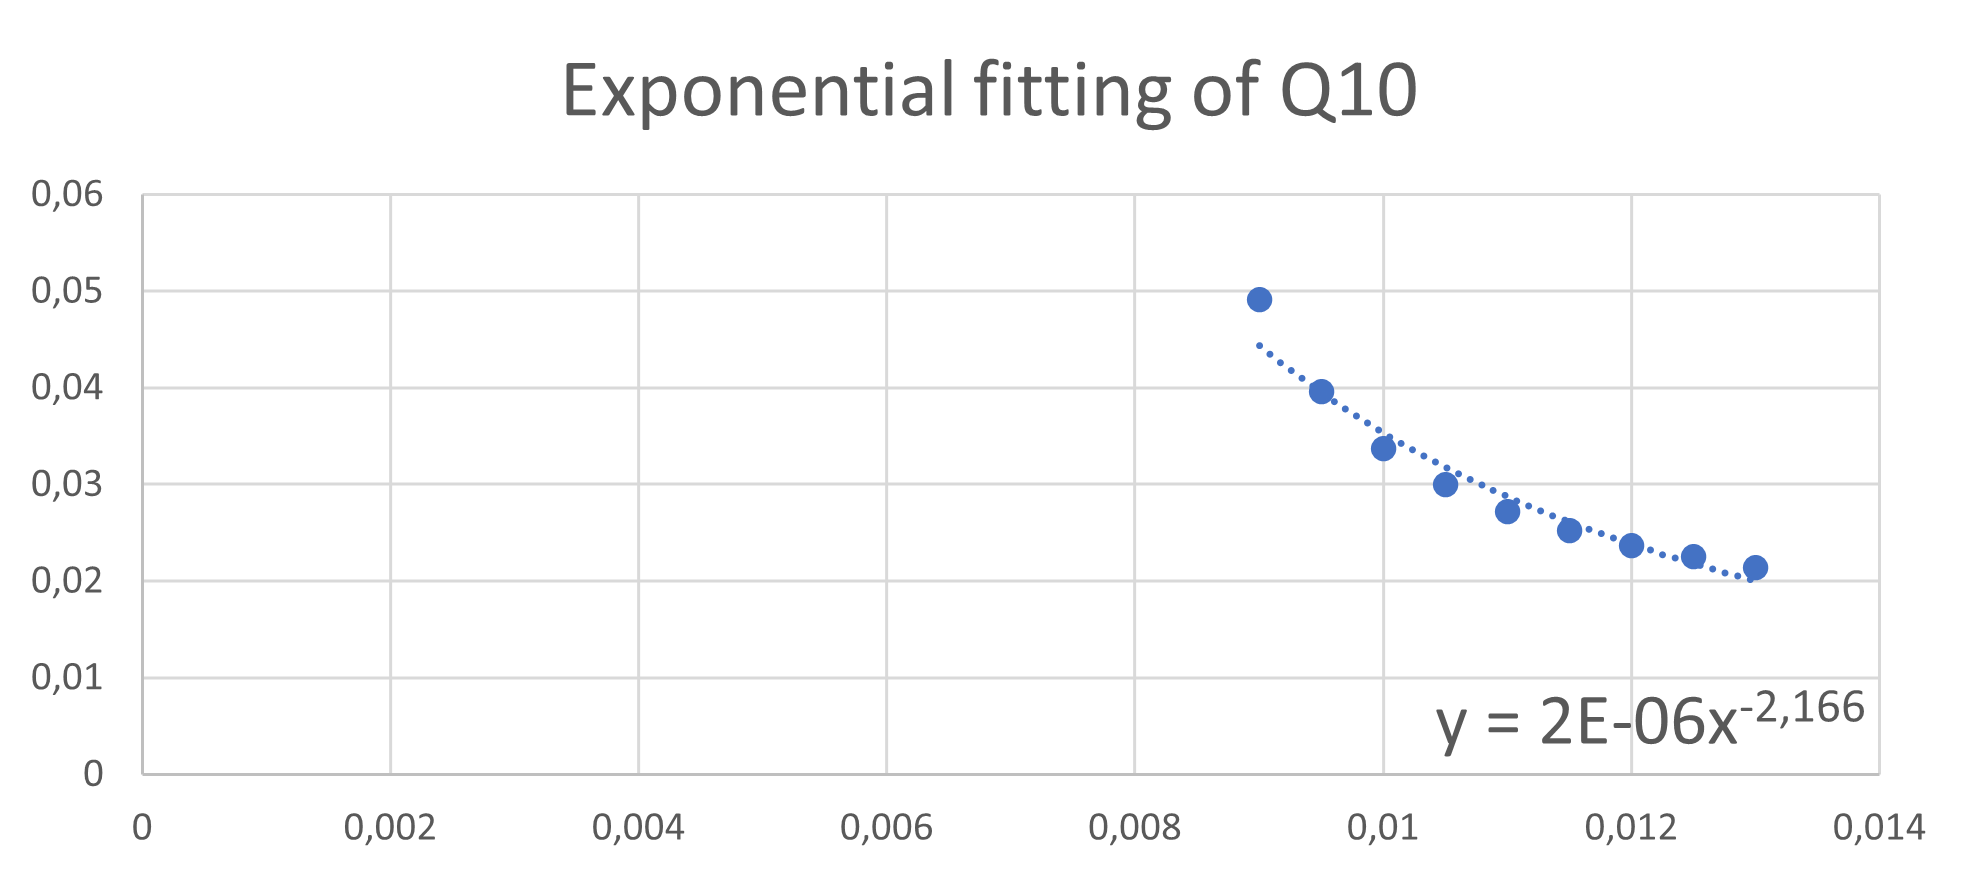
\includegraphics[width=\textwidth]{./data_analysis/Q10_exp_lambda.png}
                            \caption{Fitting with the exponential}
                            \label{fig:Q10_exp_lambda}
                        \end{minipage}
                        \hspace{10mm}
                        \begin{minipage}[c]{.40\textwidth}
                            \centering
                            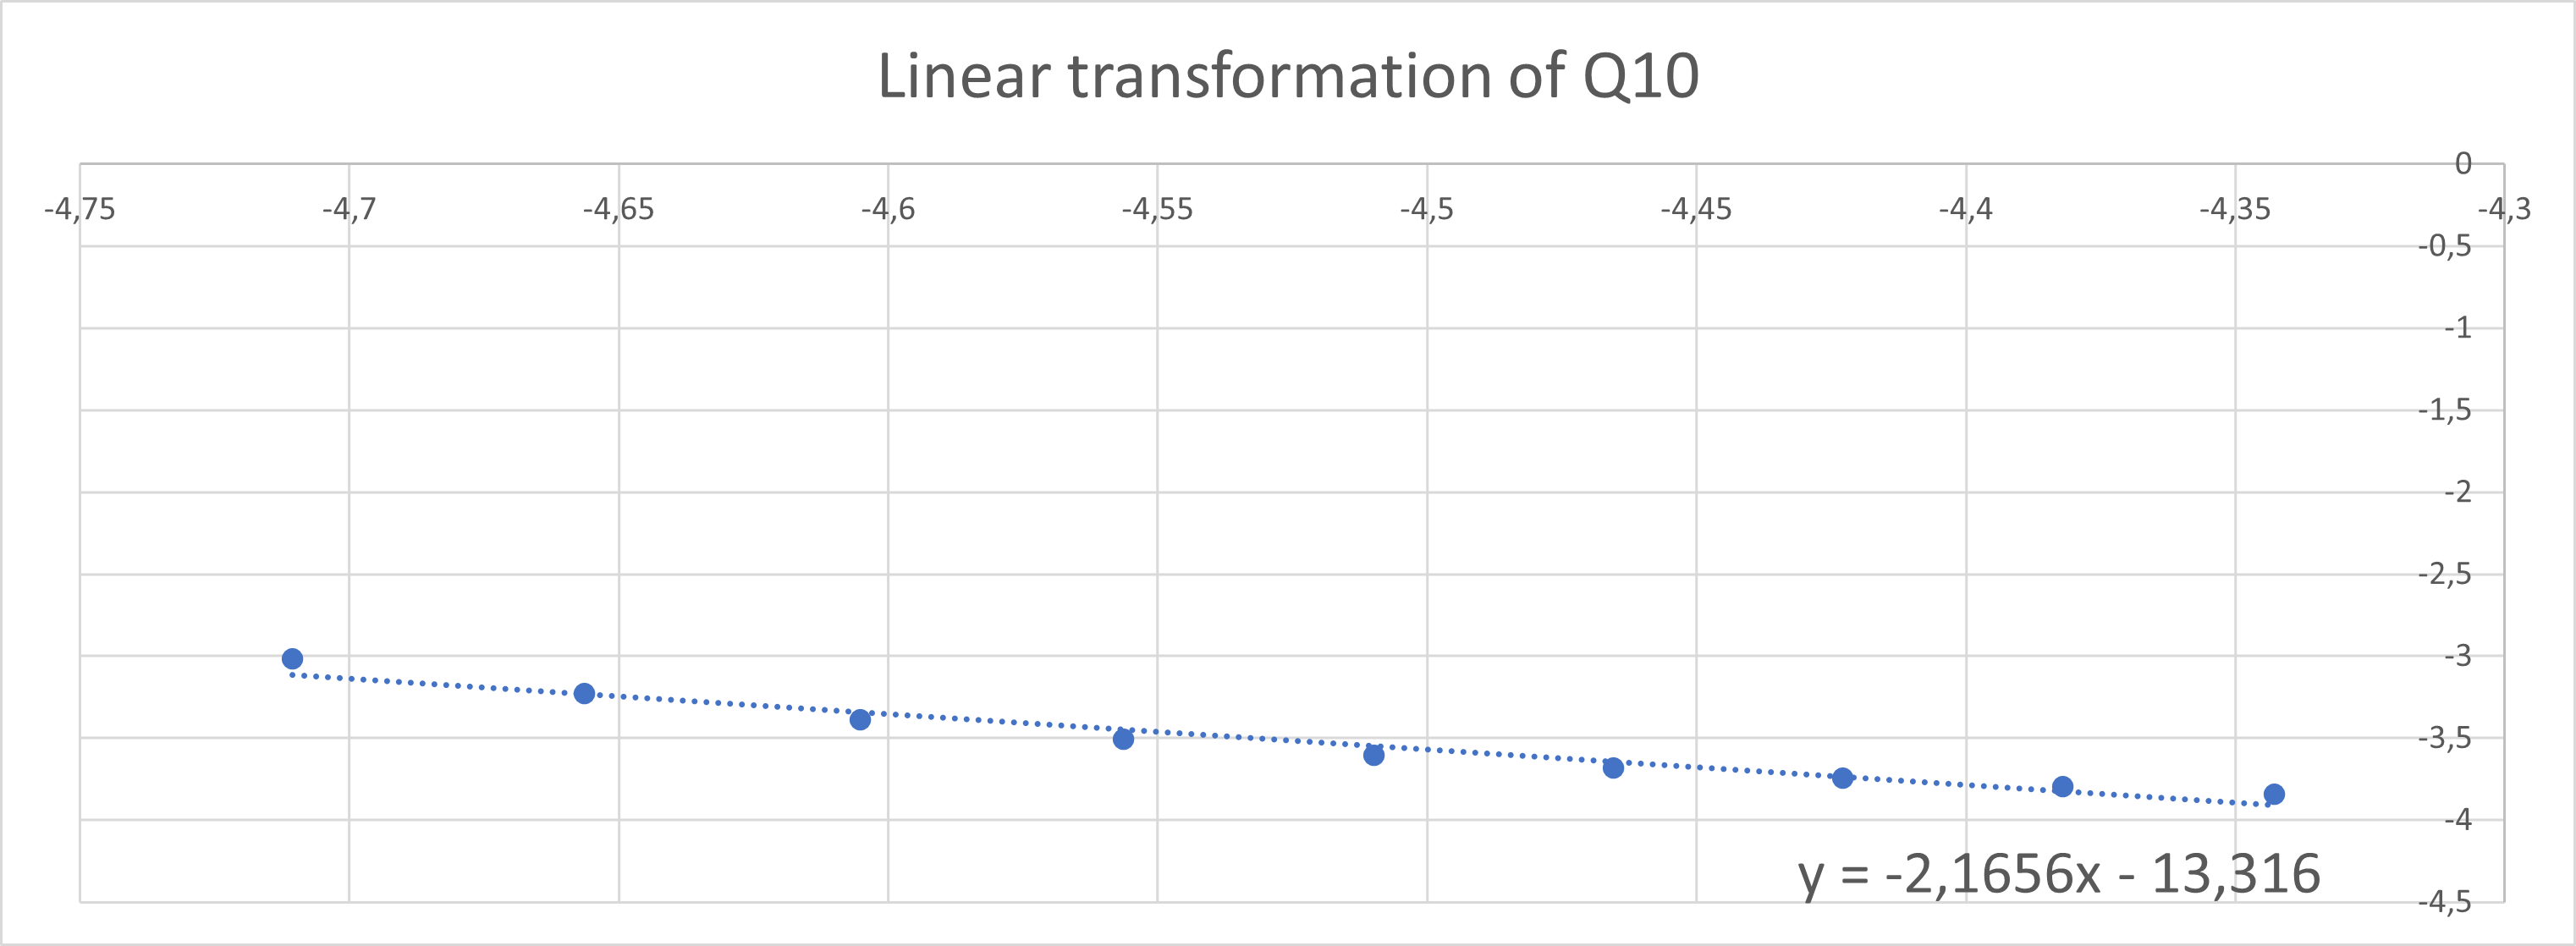
\includegraphics[width=\textwidth]{./data_analysis/Q10_lin_lambda.png}
                            \caption{Transformation of the exponential for linear regression}
                            \label{fig:Q10_lin_lambda}
                        \end{minipage}
                    \end{figure}
                    
                    \begin{table}[htbp]
                        \centering 
                        \begin{tabular}{|c|c|c|}
                            
                            \hline
                            \multicolumn{3}{|c|}{\bf Confidence interval with 95\% confidence level} \\
                            
                            \hline
                            \ & Slope & Offset\\
                            \hline
                            \ Upper Limit & -1.983521893 & -13.10149438 \\ 
                            \hline
                            \ Lower Limit & -2.347678107 & -13.53050562 \\ 
                            \hline
                        \end{tabular}
                        \label{table:CI_10_fitting_lambda}
                    \end{table}
                    
            \subsubsection{Linear regression for $\lambda\mu$}
                \paragraph{Settings for the simulations} \hfill \\
                    \lstinputlisting[language=Octave]{txt_ini/Q10_lambda_mu.txt}
                                \paragraph{Fitting} \hfill \\

                    Considering the interplay between $\lambda$ and $\mu$ we obtained once again an exponential fitting.
                    The reasons behind this behavior are the same illustrated for the case $Q = 5S_t$.
                    
                    \begin{figure}[htbp!]
                        \centering
                        \begin{minipage}[c]{.40\textwidth}
                            \centering
                            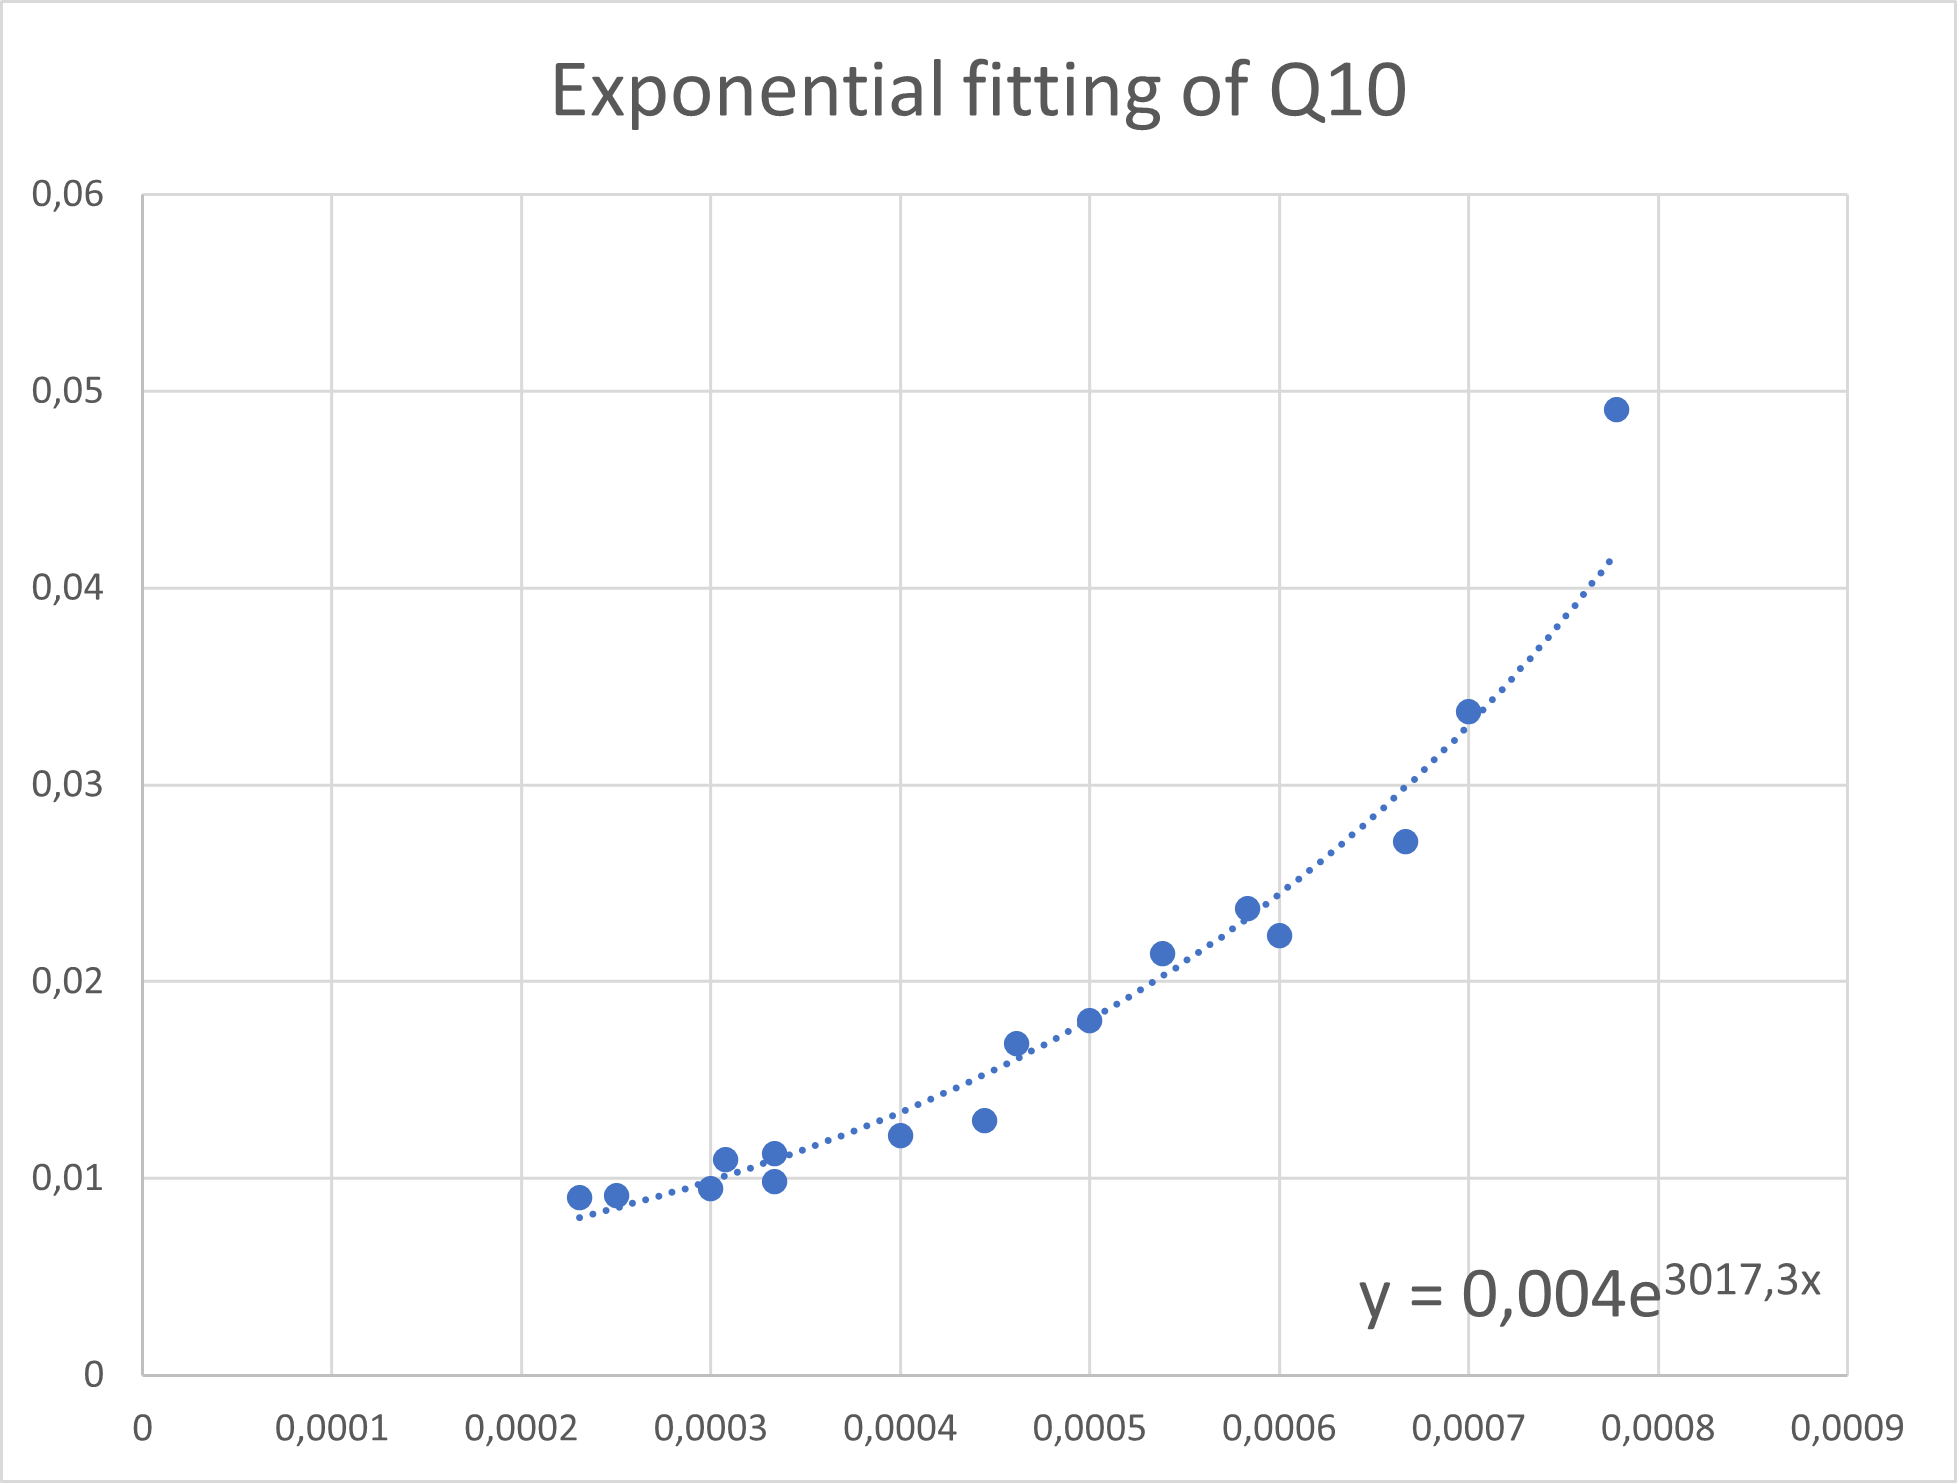
\includegraphics[width=\textwidth]{./data_analysis/Q10_exp_lambda_mu.png}
                            \caption{Fitting with the exponential}
                            \label{fig:Q10_exp_lambda_mu}
                        \end{minipage}
                        \hspace{10mm}
                        \begin{minipage}[c]{.40\textwidth}
                            \centering
                            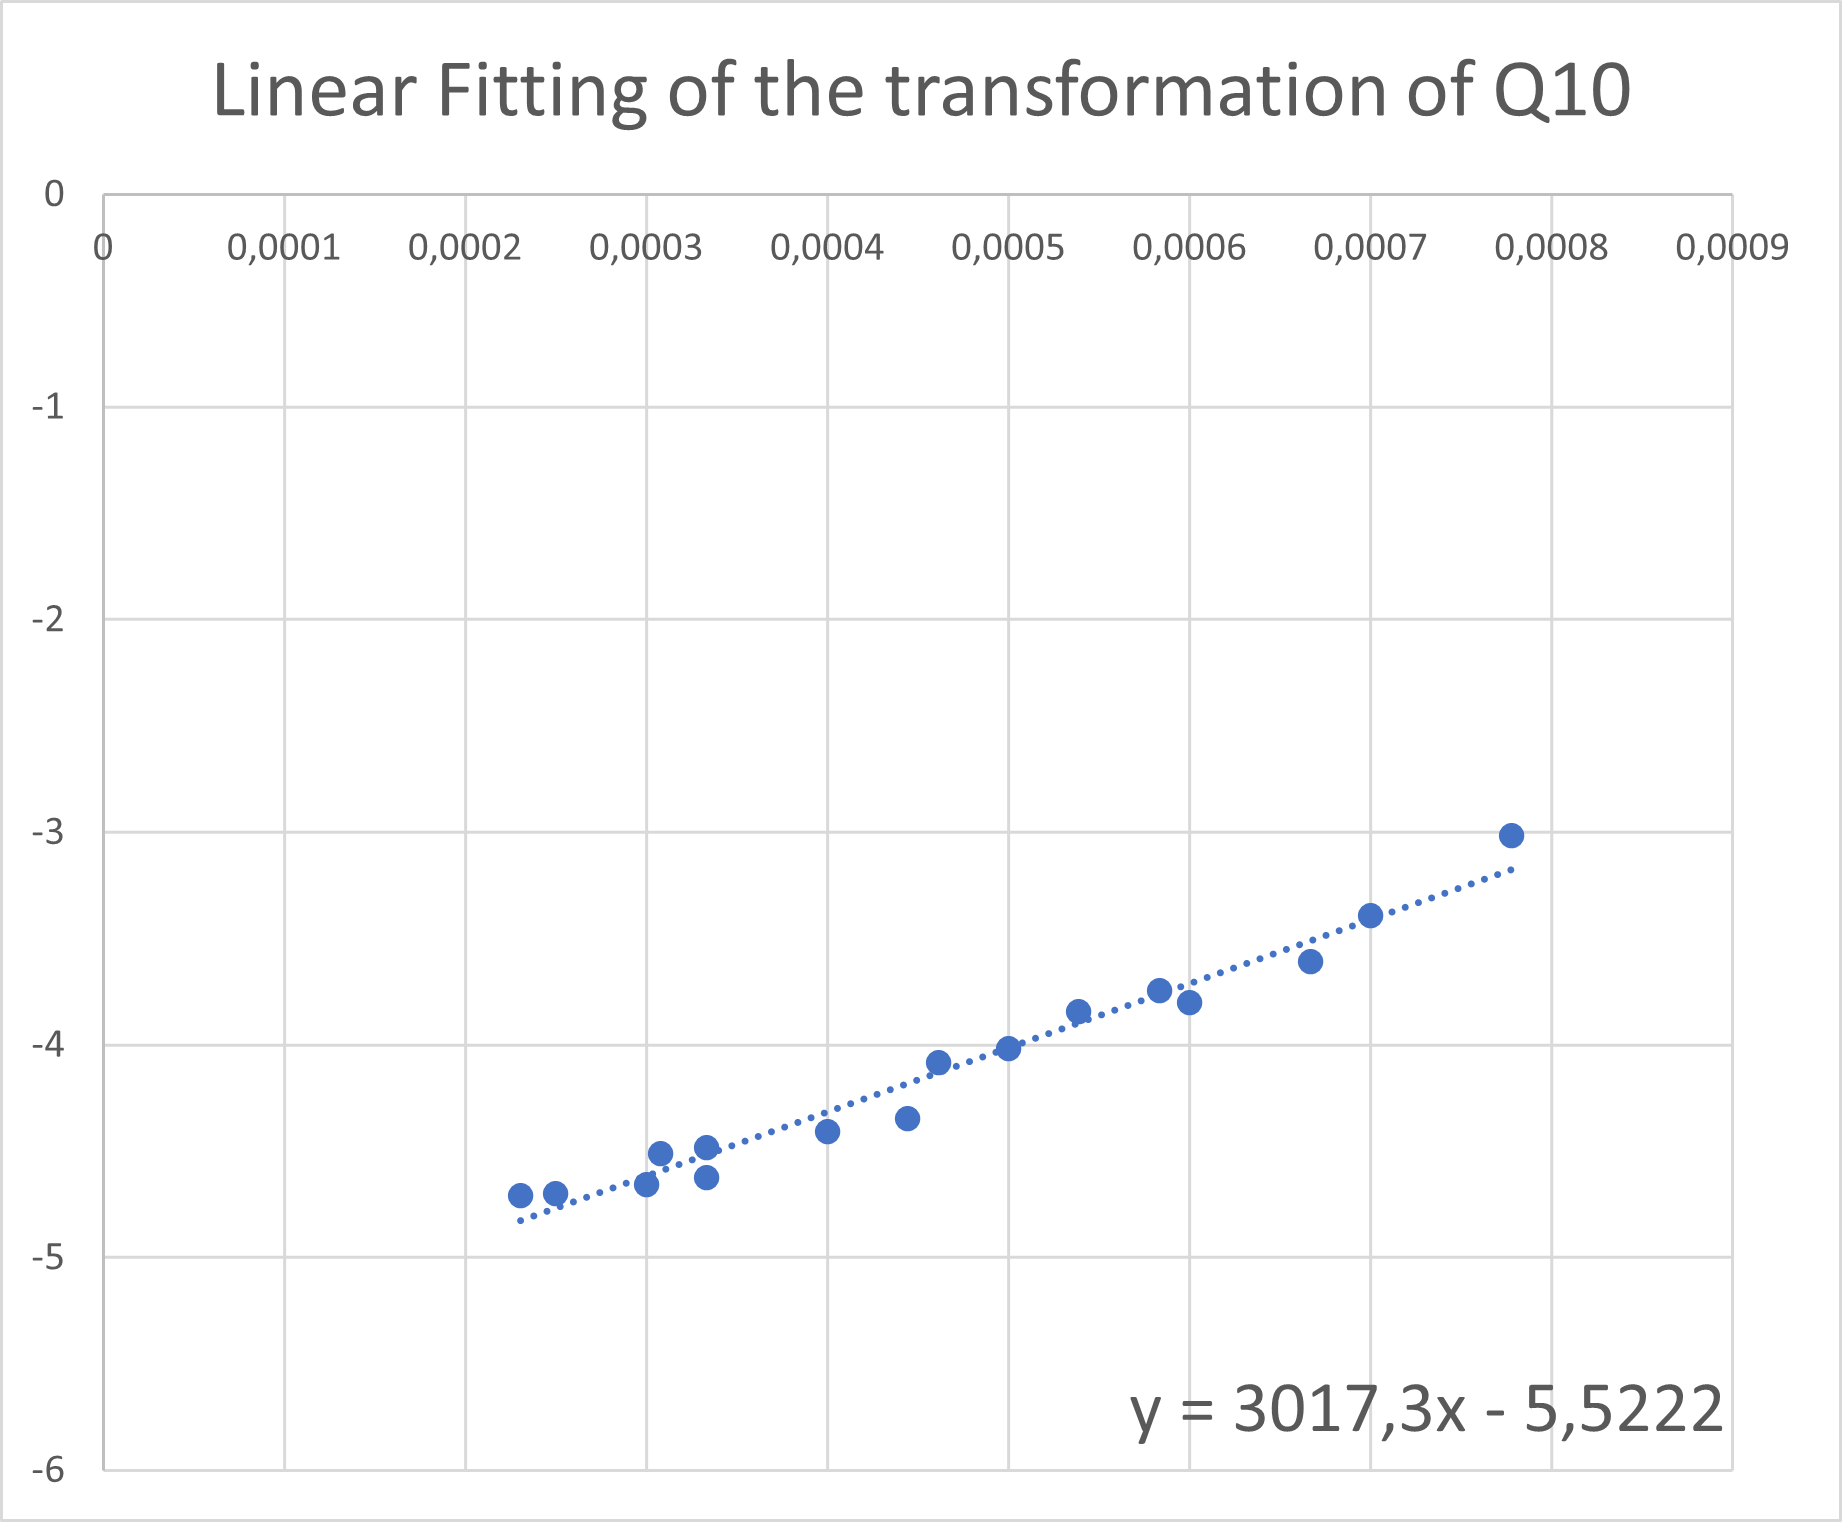
\includegraphics[width=\textwidth]{./data_analysis/Q10_lin_lambda_mu.png}
                            \caption{Transformation of the exponential for linear regression}
                            \label{fig:Q10_lin_lambda_mu}
                        \end{minipage}
                    \end{figure}
                    
                    \begin{table}[htbp]
                        \centering 
                        \begin{tabular}{|c|c|c|}
                            
                            \hline
                            \multicolumn{3}{|c|}{\bf Confidence interval with 95\% confidence level} \\
                            
                            \hline
                            \ & Slope & Offset\\
                            \hline
                            \ Upper Limit & 3017.401167 & -5.417960402 \\ 
                            \hline
                            \ Lower Limit & 3017.198833 & -5.717214431 \\ 
                            \hline
                        \end{tabular}
                        \label{table:CI_10_fitting_lambda-mu}
                    \end{table}
   \newpage                
\section{Conclusions}
    As a last consideration, we observed how our system behaves in different ways depending on the ratio between service time and turn time. When the ratio is close to $1$, the response time will depend mostly on \textit{Service time} and \textit{Vacation}, while as the ratio starts to go below one, $\delta$ will get more and more influential and $\mu$ will lose importance. This makes sense since when the ratio is really small, the server has to go on vacations many times in order to build a turn big enough to serve a job. This also explains why when we are dealing with small values of $Q$ we use very large values for the inter-arrival times in order to maintain the system stable. On the other hand, as the ratio between the turn time and service time grows bigger, the vacation becomes insignificant for what concerns the response time since the turn is big enough to serve many jobs before going on vacation while inter-arrival time and service time will impact more on the system.
           
\end{document}
